\documentclass[a4paper]{article}

%% Language and font encodings
\usepackage[english]{babel}
\usepackage[utf8]{inputenc}
\usepackage[T1]{fontenc}

%% Sets page size and margins
\usepackage[a4paper,top=2.5cm,bottom=2.5cm,left=2.5cm,right=2.5cm,marginparwidth=1.75cm]{geometry}

%% Useful packages
\usepackage{multicol}
\usepackage{paralist}
\usepackage{amsmath}
\usepackage{bm,bbm}
\usepackage{amsthm}
\usepackage{graphicx}
\usepackage[colorinlistoftodos]{todonotes}
\usepackage[colorlinks=true, allcolors=blue]{hyperref}
\usepackage{nameref,cleveref}

\usepackage{../includes/MarkMathCmds}
\allowdisplaybreaks
\usepackage{mathtools}
\newcommand{\mat}[1]{{\mathrm{{#1}}}} % matrix

\usepackage{MarkBiblatexCmds}
\addbibresource{ref.bib}

\usepackage{enumitem}
\usepackage{epsdice}
\usepackage{bbm}

% tikzlibrary.code.tex
%
% Copyright 2010-2011 by Laura Dietz
% Copyright 2012 by Jaakko Luttinen
%
% The MIT License
%
% See LICENSE file for more details.

% Load other libraries
\usetikzlibrary{shapes}
\usetikzlibrary{fit}
\usetikzlibrary{chains}
\usetikzlibrary{arrows}

% Latent node
\tikzstyle{latent} = [circle,fill=white,draw=black,inner sep=1pt,
minimum size=20pt, font=\fontsize{10}{10}\selectfont, node distance=1]
% Observed node
\tikzstyle{obs} = [latent,fill=gray!25]
% Constant node
\tikzstyle{const} = [rectangle, inner sep=0pt, node distance=1]
% Factor node
\tikzstyle{factor} = [rectangle, fill=black,minimum size=5pt, inner
sep=0pt, node distance=0.4]
% Deterministic node
\tikzstyle{det} = [latent, diamond]

% Plate node
\tikzstyle{plate} = [draw, rectangle, rounded corners, fit=#1]
% Invisible wrapper node
\tikzstyle{wrap} = [inner sep=0pt, fit=#1]
% Gate
\tikzstyle{gate} = [draw, rectangle, dashed, fit=#1]

% Caption node
\tikzstyle{caption} = [font=\footnotesize, node distance=0] %
\tikzstyle{plate caption} = [caption, node distance=0, inner sep=0pt,
below left=5pt and 0pt of #1.south east] %
\tikzstyle{factor caption} = [caption] %
\tikzstyle{every label} += [caption] %

%\pgfdeclarelayer{b}
%\pgfdeclarelayer{f}
%\pgfsetlayers{b,main,f}

% \factoredge [options] {inputs} {factors} {outputs}
\newcommand{\factoredge}[4][]{ %
  % Connect all nodes #2 to all nodes #4 via all factors #3.
  \foreach \f in {#3} { %
    \foreach \x in {#2} { %
      \path (\x) edge[-,#1] (\f) ; %
      %\draw[-,#1] (\x) edge[-] (\f) ; %
    } ;
    \foreach \y in {#4} { %
      \path (\f) edge[->, >={triangle 45}, #1] (\y) ; %
      %\draw[->,#1] (\f) -- (\y) ; %
    } ;
  } ;
}

% \edge [options] {inputs} {outputs}
\newcommand{\edge}[3][]{ %
  % Connect all nodes #2 to all nodes #3.
  \foreach \x in {#2} { %
    \foreach \y in {#3} { %
      \path (\x) edge [->, >={triangle 45}, #1] (\y) ;%
      %\draw[->,#1] (\x) -- (\y) ;%
    } ;
  } ;
}

% \factor [options] {name} {caption} {inputs} {outputs}
\newcommand{\factor}[5][]{ %
  % Draw the factor node. Use alias to allow empty names.
  \node[factor, label={[name=#2-caption]#3}, name=#2, #1,
  alias=#2-alias] {} ; %
  % Connect all inputs to outputs via this factor
  \factoredge {#4} {#2-alias} {#5} ; %
}

% \plate [options] {name} {fitlist} {caption}
\newcommand{\plate}[4][]{ %
  \node[wrap=#3] (#2-wrap) {}; %
  \node[plate caption=#2-wrap] (#2-caption) {#4}; %
  \node[plate=(#2-wrap)(#2-caption), #1] (#2) {}; %
}

% \gate [options] {name} {fitlist} {inputs}
\newcommand{\gate}[4][]{ %
  \node[gate=#3, name=#2, #1, alias=#2-alias] {}; %
  \foreach \x in {#4} { %
    \draw [-*,thick] (\x) -- (#2-alias); %
  } ;%
}

% \vgate {name} {fitlist-left} {caption-left} {fitlist-right}
% {caption-right} {inputs}
\newcommand{\vgate}[6]{ %
  % Wrap the left and right parts
  \node[wrap=#2] (#1-left) {}; %
  \node[wrap=#4] (#1-right) {}; %
  % Draw the gate
  \node[gate=(#1-left)(#1-right)] (#1) {}; %
  % Add captions
  \node[caption, below left=of #1.north ] (#1-left-caption)
  {#3}; %
  \node[caption, below right=of #1.north ] (#1-right-caption)
  {#5}; %
  % Draw middle separation
  \draw [-, dashed] (#1.north) -- (#1.south); %
  % Draw inputs
  \foreach \x in {#6} { %
    \draw [-*,thick] (\x) -- (#1); %
  } ;%
}

% \hgate {name} {fitlist-top} {caption-top} {fitlist-bottom}
% {caption-bottom} {inputs}
\newcommand{\hgate}[6]{ %
  % Wrap the left and right parts
  \node[wrap=#2] (#1-top) {}; %
  \node[wrap=#4] (#1-bottom) {}; %
  % Draw the gate
  \node[gate=(#1-top)(#1-bottom)] (#1) {}; %
  % Add captions
  \node[caption, above right=of #1.west ] (#1-top-caption)
  {#3}; %
  \node[caption, below right=of #1.west ] (#1-bottom-caption)
  {#5}; %
  % Draw middle separation
  \draw [-, dashed] (#1.west) -- (#1.east); %
  % Draw inputs
  \foreach \x in {#6} { %
    \draw [-*,thick] (\x) -- (#1); %
  } ;%
}


% Copyright (C) 2016  Joseph Rabinoff

% ipe2tikz is free software; you can redistribute it and/or modify it under
% the terms of the GNU General Public License as published by the Free
% Software Foundation; either version 3 of the License, or (at your option)
% any later version.

% ipe2tikz is distributed in the hope that it will be useful, but WITHOUT ANY
% WARRANTY; without even the implied warranty of MERCHANTABILITY or FITNESS
% FOR A PARTICULAR PURPOSE.  See the GNU General Public License for more
% details.

% You should have received a copy of the GNU General Public License along with
% ipe2tikz; if not, you can find it at "http://www.gnu.org/copyleft/gpl.html",
% or write to the Free Software Foundation, Inc., 675 Mass Ave, Cambridge, MA
% 02139, USA.


% ipe compatibility TikZ styles

\usetikzlibrary{arrows.meta}

\makeatletter

% These should behave almost exactly like ipe arrows.  They disable correcting
% for the miter length and line width.  This is important for visual consistency
% with ipe, since ipe arrows get much larger when the line width is increased.
% They also use the line join and cap styles from the main path.  These are very
% simple arrows: there is no harpoon version, and the convex hull computation is
% sloppy.

\pgfdeclarearrow{
  name = ipe _linear,
  defaults = {
    length = +1bp,
    width  = +.666bp,
    line width = +0pt 1,
  },
  setup code = {
    % Control points
    \pgfarrowssetbackend{0pt}
    \pgfarrowssetvisualbackend{
      \pgfarrowlength\advance\pgf@x by-.5\pgfarrowlinewidth}
    \pgfarrowssetlineend{\pgfarrowlength}
    \ifpgfarrowreversed
      \pgfarrowssetlineend{\pgfarrowlength\advance\pgf@x by-.5\pgfarrowlinewidth}
    \fi
    \pgfarrowssettipend{\pgfarrowlength}
    % Convex hull
    \pgfarrowshullpoint{\pgfarrowlength}{0pt}
    \pgfarrowsupperhullpoint{0pt}{.5\pgfarrowwidth}
    % The following are needed in the code:
    \pgfarrowssavethe\pgfarrowlinewidth
    \pgfarrowssavethe\pgfarrowlength
    \pgfarrowssavethe\pgfarrowwidth
  },
  drawing code = {
    \pgfsetdash{}{+0pt}
    \ifdim\pgfarrowlinewidth=\pgflinewidth\else\pgfsetlinewidth{+\pgfarrowlinewidth}\fi
    \pgfpathmoveto{\pgfqpoint{0pt}{.5\pgfarrowwidth}}
    \pgfpathlineto{\pgfqpoint{\pgfarrowlength}{0pt}}
    \pgfpathlineto{\pgfqpoint{0pt}{-.5\pgfarrowwidth}}
    \pgfusepathqstroke
  },
  parameters = {
    \the\pgfarrowlinewidth,%
    \the\pgfarrowlength,%
    \the\pgfarrowwidth,%
  },
}


\pgfdeclarearrow{
  name = ipe _pointed,
  defaults = {
    length = +1bp,
    width  = +.666bp,
    inset  = +.2bp,
    line width = +0pt 1,
  },
  setup code = {
    % Control points
    \pgfarrowssetbackend{0pt}
    \pgfarrowssetvisualbackend{\pgfarrowinset}
    \pgfarrowssetlineend{\pgfarrowinset}
    \ifpgfarrowreversed
      \pgfarrowssetlineend{\pgfarrowlength}
    \fi
    \pgfarrowssettipend{\pgfarrowlength}
    % Convex hull
    \pgfarrowshullpoint{\pgfarrowlength}{0pt}
    \pgfarrowsupperhullpoint{0pt}{.5\pgfarrowwidth}
    \pgfarrowshullpoint{\pgfarrowinset}{0pt}
    % The following are needed in the code:
    \pgfarrowssavethe\pgfarrowinset
    \pgfarrowssavethe\pgfarrowlinewidth
    \pgfarrowssavethe\pgfarrowlength
    \pgfarrowssavethe\pgfarrowwidth
  },
  drawing code = {
    \pgfsetdash{}{+0pt}
    \ifdim\pgfarrowlinewidth=\pgflinewidth\else\pgfsetlinewidth{+\pgfarrowlinewidth}\fi
    \pgfpathmoveto{\pgfqpoint{\pgfarrowlength}{0pt}}
    \pgfpathlineto{\pgfqpoint{0pt}{.5\pgfarrowwidth}}
    \pgfpathlineto{\pgfqpoint{\pgfarrowinset}{0pt}}
    \pgfpathlineto{\pgfqpoint{0pt}{-.5\pgfarrowwidth}}
    \pgfpathclose
    \ifpgfarrowopen
      \pgfusepathqstroke
    \else
      \ifdim\pgfarrowlinewidth>0pt\pgfusepathqfillstroke\else\pgfusepathqfill\fi
    \fi
  },
  parameters = {
    \the\pgfarrowlinewidth,%
    \the\pgfarrowlength,%
    \the\pgfarrowwidth,%
    \the\pgfarrowinset,%
    \ifpgfarrowopen o\fi%
  },
}


% For correcting minipage width in stretched nodes
\newdimen\ipeminipagewidth
\def\ipestretchwidth#1{%
  \pgfmathsetlength{\ipeminipagewidth}{#1/\ipenodestretch}}

\tikzstyle{ipe import} = [
  % General ipe defaults
  x=1bp, y=1bp,
%
  % Nodes
  ipe node stretch/.store in=\ipenodestretch,
  ipe stretch normal/.style={ipe node stretch=1},
  ipe stretch normal,
  ipe node/.style={
    anchor=base west, inner sep=0, outer sep=0, scale=\ipenodestretch
  },
%
  % Use a special key for the mark scale, so that the default can be overriden.
  % (This doesn't happen with the scale= key; those accumulate.)
  ipe mark scale/.store in=\ipemarkscale,
%
  ipe mark tiny/.style={ipe mark scale=1.1},
  ipe mark small/.style={ipe mark scale=2},
  ipe mark normal/.style={ipe mark scale=3},
  ipe mark large/.style={ipe mark scale=5},
%
  ipe mark normal, % Set default
%
  ipe circle/.pic={
    \draw[line width=0.2*\ipemarkscale]
      (0,0) circle[radius=0.5*\ipemarkscale];
    \coordinate () at (0,0);
  },
  ipe disk/.pic={
    \fill (0,0) circle[radius=0.6*\ipemarkscale];
    \coordinate () at (0,0);
  },
  ipe fdisk/.pic={
    \filldraw[line width=0.2*\ipemarkscale]
      (0,0) circle[radius=0.5*\ipemarkscale];
    \coordinate () at (0,0);
  },
  ipe box/.pic={
    \draw[line width=0.2*\ipemarkscale, line join=miter]
      (-.5*\ipemarkscale,-.5*\ipemarkscale) rectangle
      ( .5*\ipemarkscale, .5*\ipemarkscale);
    \coordinate () at (0,0);
  },
  ipe square/.pic={
    \fill
      (-.6*\ipemarkscale,-.6*\ipemarkscale) rectangle
      ( .6*\ipemarkscale, .6*\ipemarkscale);
    \coordinate () at (0,0);
  },
  ipe fsquare/.pic={
    \filldraw[line width=0.2*\ipemarkscale, line join=miter]
      (-.5*\ipemarkscale,-.5*\ipemarkscale) rectangle
      ( .5*\ipemarkscale, .5*\ipemarkscale);
    \coordinate () at (0,0);
  },
  ipe cross/.pic={
    \draw[line width=0.2*\ipemarkscale, line cap=butt]
      (-.5*\ipemarkscale,-.5*\ipemarkscale) --
      ( .5*\ipemarkscale, .5*\ipemarkscale)
      (-.5*\ipemarkscale, .5*\ipemarkscale) --
      ( .5*\ipemarkscale,-.5*\ipemarkscale);
    \coordinate () at (0,0);
  },
%
  % Arrow sizes (for TikZ arrows)
  /pgf/arrow keys/.cd,
  ipe arrow normal/.style={scale=1},
  ipe arrow tiny/.style={scale=.4},
  ipe arrow small/.style={scale=.7},
  ipe arrow large/.style={scale=1.4},
  ipe arrow normal,
  /tikz/.cd,
%
  % Approximations to ipe arrows
  % Put in a style to allow to reset default scale when "ipe arrow normal" is
  % changed.  I think this is the only way, since all the parameters to arrows
  % are expanded when the tip is declared.
  ipe arrows/.style={
    ipe normal/.tip={
      ipe _pointed[length=1bp, width=.666bp, inset=0bp,
                   quick, ipe arrow normal]},
    ipe pointed/.tip={
      ipe _pointed[length=1bp, width=.666bp, inset=0.2bp,
                   quick, ipe arrow normal]},
    ipe linear/.tip={
      ipe _linear[length = 1bp, width=.666bp,
                  ipe arrow normal, quick]},
    ipe fnormal/.tip={ipe normal[fill=white]},
    ipe fpointed/.tip={ipe pointed[fill=white]},
    ipe double/.tip={ipe normal[] ipe normal},
    ipe fdouble/.tip={ipe fnormal[] ipe fnormal},
    % These should maybe use [bend], but that often looks bad unless it's on an
    % actual arc.
    ipe arc/.tip={ipe normal},
    ipe farc/.tip={ipe fnormal},
    ipe ptarc/.tip={ipe pointed},
    ipe fptarc/.tip={ipe fpointed},
  },
  ipe arrows, % Set default sizes
]

% I'm not sure how to do this in a .style, since the #args get confused.
\tikzset{
  rgb color/.code args={#1=#2}{%
    \definecolor{tempcolor-#1}{rgb}{#2}%
    \tikzset{#1=tempcolor-#1}%
  },
}

\makeatother

\endinput



\newcommand{\bo}{\omega}
%\newcommand{\KL}{\text{KL}}
\newcommand{\train}{\text{train}}
\newcommand{\D}{\mathcal{D}}
\newcommand{\softmax}{\text{Softmax}}

\newcommand{\logsumexp}{\text{log-sum-exp}}

\newcommand{\vfe}{\mathcal{F}_{\text{VI}}}
\newcommand{\snr}{\text{SNR}}

\newcommand{\R}{\mathbb{R}}
\newcommand{\N}{\mathcal{N}}
\newcommand{\cL}{\mathcal{L}}
\newcommand{\cO}{\mathcal{O}}
\newcommand{\svert}{~|~}
\newcommand{\td}{\text{d}}
\newcommand{\f}{\mathbf{f}}
\newcommand{\x}{\mathbf{x}}
\newcommand{\Bb}{\mathbf{b}}
%\newcommand{\sBb}{\mathtt{b}}
\newcommand{\sBb}{\mathtt{z}}
\newcommand{\bx}{\overline{\x}}
\newcommand{\bb}{\overline{b}}
\newcommand{\y}{\mathbf{y}}
\newcommand{\z}{\mathbf{z}}
\newcommand{\bu}{\mathbf{u}}
\newcommand{\bv}{\mathbf{v}}
\newcommand{\bV}{\mathbf{V}}
\newcommand{\bU}{\mathbf{U}}
\newcommand{\bk}{\mathbf{k}}
\newcommand{\w}{\mathbf{w}}
\newcommand{\W}{\mathbf{W}}
\newcommand{\ba}{\mathbf{a}}
\newcommand{\m}{\mathbf{m}}
\newcommand{\ls}{\mathbf{l}}
\newcommand{\bL}{\mathbf{L}}
\newcommand{\A}{\mathbf{A}}
\newcommand{\X}{\mathbf{X}}
\newcommand{\Z}{\mathbf{Z}}
\newcommand{\BS}{\mathbf{S}}
%\newcommand{\BA}{\mathbf{A}}
\newcommand{\BP}{\mathbf{P}}
\newcommand{\BQ}{\mathbf{Q}}
\newcommand{\Y}{\mathbf{Y}}
\newcommand{\F}{\mathbf{F}}
%\newcommand{\I}{\mathbf{I}}
\newcommand{\M}{\mathbf{M}}
\newcommand{\bp}{\overline{\p}}
\newcommand{\bz}{\mathbf{0}}
\newcommand{\bepsilon}{\text{\boldmath$\epsilon$}}
\newcommand{\bgamma}{\text{\boldmath$\gamma$}}
\newcommand{\s}{\mathbf{s}}
\newcommand{\Unif}{\text{Unif}}
\newcommand{\boh}{\widehat{\text{\boldmath$\omega$}}}
\newcommand{\bsigma}{\text{\boldmath$\sigma$}}
\newcommand{\bSigma}{\text{\boldmath$\Sigma$}}
\newcommand{\bmu}{\text{\boldmath$\mu$}}
\newcommand{\bphi}{\text{\boldmath$\phi$}}
\newcommand{\Kh}{\widehat{\mathbf{K}}}
\newcommand{\tr}{\text{tr}}
\newcommand{\tdet}{\text{det}}
% \newcommand{\KL}{\text{KL}}
\newcommand{\ind}{\mathds{1}}
\newcommand{\bc}{\mathbf{c}}
\newcommand{\reg}{\eta}
\newcommand{\weightdecay}{\lambda}
\newcommand{\h}{\mathbf{h}}

% variables
\newcommand{\mparam}{\bm{\theta}}	% model param
\newcommand{\vparam}{\bm{\phi}}	% variational param

% gradient approximation part
\newcommand{\hparam}{\bm{\varphi}}
\newcommand{\Xb}{\mathbb{X}}
\newcommand{\hgrad}{\overline{\nabla_{\x} \h}}
\newcommand{\Hmatrix}{\mathbf{H}}
\newcommand{\Grad}{\mathbf{G}}
\newcommand{\g}{\bm{g}}
\newcommand{\noise}{\bm{\epsilon}}


\newcommand{\mx}{\vm_\vx}
\newcommand{\my}{\vm_\vy}
\newcommand{\covmat}{\boldsymbol{\Sigma}}
\newcommand{\covx}{\boldsymbol{\Sigma}_{\vx\vx}}
\newcommand{\covy}{\boldsymbol{\Sigma}_{\vy\vy}}
\newcommand{\covxy}{\boldsymbol{\Sigma}_{\vx\vy}}
\newcommand{\covyx}{\boldsymbol{\Sigma}_{\vy\vx}}

\newcommand{\K}{\mathbf{K}}

\newcommand{\questionref}[1]{\Cref{#1} -- \nameref{#1}}

\newcommand{\lb}{\mathcal{L}}
\newcommand{\sumn}{\sum_{n=1}^N}

\newcommand{\dA}{\epsdice{1}}
\newcommand{\dB}{\epsdice{2}}
\newcommand{\dC}{\epsdice{3}}
\newcommand{\dD}{\epsdice{4}}
\newcommand{\dE}{\epsdice{5}}
\newcommand{\dF}{\epsdice{6}}

\theoremstyle{definition}
\newtheorem{question}{Question}

\newcommand{\courseprobstats}{\texttt{50008} \textit{Probability \& Statistics}}


\title{70015 Mathematics for Machine Learning: Exercises}
\author{Mark van der Wilk, Yingzhen Li\footnote{Many thanks to teaching assistants Carles Balsells Rodas, and Alex Spies for their solutions and improvements to the document.} \\ \texttt{\{m.vdwilk,yingzhen.li\}@imperial.ac.uk}}



\begin{document}
\maketitle
\tableofcontents



% \section{Background material}\todo{Adjust.}
% You will be expected to have a \emph{firm} understanding of Mathematics for Machine Learning. In the explanations, I will be manipulating probabilities and expectations freely, as discussed in Mathematics for Machine Learning. If steps are difficult, I encourage you to raise this on the course EdStem page, or during a Q\&A session.

% \begin{itemize}
% \item Basic probability: sample spaces, disjoint events (summation of probabilities), independent events (multiplication of probabilities). See \citet{walpole2012probability}, Ch2 (Imperial Library, or search Google for reading options).
% \item Probability densities. See \citet{mml} \S 6.2.
% \item Sum, product \& Bayes' rules. See \citet{mml} \S 6.3.
% \item Unconstrained continuous optimisation. See \citet{mml} \S 7.1.
% \item Linear algebra and matrix decompositions. See \citet{mml} ch 4 (and Chs 2 and 3 for basics).
% \item A familiarity with linear basis-function regression. See \citet{mml} ch 9.
% \end{itemize}


\section{Notation}
\subsection{Sets}
Throughout this course, we will be using some standard mathematical notation which may be unfamiliar to some. It's ultimately not that special or even crucial to the overall argument, but it is compact (which is practical), and it helps somewhat with practising with expressing things mathematically. Wikipedia has good definitions on these things too.
\begin{itemize}
\item Notation referring to sets of numbers, e.g.~the natural numbers $\mathbb N = \{0, 1, 2, \dots\}$, integers $\mathbb Z = \{\dots, -2, -1, 0, 1, 2, \dots\}$, or real numbers $\mathbb R$.
\item Vectors are sets containing $n$ of some type of object, like reals. We denote the set of all such sets using a superscript notation. For example, all $n$-dimensional vectors becomes $\mathbb R^n$.
\item With $x \in \mathcal S$ we denote that $x$ is an element of the set $\mathcal S$. This allows us to specify that a variable comes from a particular set (or, has a particular type), e.g.~$x \in \Reals^D$.
\item We sometimes use ``set builder'' notation. We did this informally above when defining $\mathbb N$! Usually this works by specifying elements with some property, e.g.~$\mathbf S = \{2n \,|\, n \in \mathbb N\}$, which means ``all the elements 2n such that $n$ is a natural number''. This creates the set of all even positive whole numbers.
\item We denote the union of two sets (the set with all elements that are in either set or both) as $A \cup B$. With set-builder notation this is $A \cup B = \{x\,|\,x\in A \vee x\in B\}$, where $\vee$ means ``or''.
\item We denote the intersection of two sets (the set of all elements that are in both stes) as $A \cap B = \{x\,|\,x\in A \wedge x\in B\}$.
\item For intervals of real numbers, we use brackets, $[,]$, to denote the elements in the set which are "greater than or equal to" and "less than or equal to" an element, respectively. We use parentheses, $(,)$ to denote a strict lower bound or upper bound on the set, respectively. E.g. $[1,5)$ is equivalent to $1 \leq x < 5, x\in\mathbb{R}$.
\item We use the symbol $\neg$ to denote the complement of a set. Given a set containing all elements under consideration $\Omega$, $\neg A$ contains all elements of $\Omega$ that are not in $A$, i.e.~$\neg A = \{x \in \Omega | x \notin A\}$. We can also denote this as $\neg A = \Omega\backslash A$.
\end{itemize}

\subsection{Probabilities}
In this course we will use the notation for probabilities that is common in machine learning. The main advantage is that this notation is shorter, although it does leave certain things implicit. We include this to reduce confusion.

Consider a probability space $(\Omega, \mathcal E, \mathbb P)$ with sample space $\Omega$ (all possible outcomes of a random procedure), event space $\mathcal E$ (the set of all sets of outcomes that we assign a probability to), and probability function $\mathbb P : \mathcal E \to [0, 1]$ (a function that assigns a probability to an event), with a random variable $X: \Omega \to \Reals^D$.
\begin{itemize}
\item With $\prob{E}$ we denote the probability of an event $E \in \mathcal E$, where $E$ is a set of outcomes.
\item Following the usual convention, we use the same notation when considering random variables, e.g.~$\prob{X < 2}$ is short for $\prob{\{s \in \Omega : X(s) < 2\}}$ (see \S6.1 in \courseprobstats).
\item We usually work directly with random variables, and specify all properties using a probability mass function (pmf) or probability density function (pdf). For a specific outcome of the random variable $\alpha$, we write:
\begin{align}
    &\prob{X=\alpha} = p_X(\alpha) && \text{for a pmf } p_X(\cdot) \,, \\
    &\prob{X \in [a, b]} = \int_a^b p_X(\alpha) d\alpha && \text{for a pdf $p_X(\cdot)$ with $\alpha \in \Reals$} \,, \\
    &\prob{X \in A} = \int_A p_X(\alpha) d\alpha && \text{for a pdf $p_X(\cdot)$ with $\alpha \in \Reals^D$}
    \,.
\end{align}
\item Sometimes we may write vectors in boldface, i.e.~$\mathbf x \in \Reals^D$. We won't always though, so keep track of how we define variables!
\item We generally denote outcomes of random variables without referring explicitly to the random variable itself. For example, when we refer to an outcome $\vx$, we implicitly know there is a random variable that can take this value. We usually denote this as the capital, for example here $X$.
\item Sometimes we abuse notation, and drop the random variable when denoting distributions when the argument of the function identifies it, e.g.~$p(\vx) = p_X(\vx)$.
\item If we want to be explicit about the random variable that we are evaluating the density/mass of, I will write e.g.~$p_{X,Y}(\vx,\vy) = p_{X|Y}(\vx|\vy)p_Y(\vy)$.
\item Expectations can be denoted in two ways:
\begin{align}
    &\Exp{X}{f(X)} && \text{to emphasise that X is random, if it is clear what its distribution is}\,, \\
    &\Exp{p(\vx)}{f(\vx)} && \text{to emphasise that we will be integrating over the distribution $p(\vx)$} \,.
\end{align}
In both cases this corresponds to the integral $\int p(\vx) f(\vx) \calcd\vx$.
\item Often, densities and pmfs can be discussed in exactly the same way, if we think of the density of a discrete RV as a sum of delta functions. I.e.~$p(\vx) = \sum_{o} \delta(\vx - \vx_o) p_o$, where $\{\vx_o\}$ is the set of discrete possible outcomes that $X$ can take, and $p_o$ are their corresponding probabilities. This allows us to write an expectation as an integral, regardless of whether the RV is continuous or discrete, because for discrete RVs we get:
\begin{align}
\Exp{p(\vx)}{f(\vx)} = \int p(\vx) f(\vx) \calcd\vx = \int \sum_o \delta(\vx - \vx_o) p_o f(\vx) \calcd\vx = \sum_o f(\vx_o)p_o \,.
\end{align}
(A delta function has the property that $\int_A \delta(\vx) \calcd\vx$ is 1 if $0 \in A$, and 0 otherwise. Linearity of integrals still holds. It can often be seen as the limit of a Gaussian distribution with zero variance.)
\end{itemize}


\section{Formula Sheet}
\begin{itemize}
\item Expectation identities for $X \in \Reals^D, Y \in \Reals^E$.
\begin{align}
\Exp{X}{AX} &= \Exp{X}{AX} = A\Exp{X}{X} \\
\Var{X}{X} &= \Exp{X}{XX\transpose} - \Exp{X}{X}\Exp{X}{X}\transpose \\
\Var{X}{AX} &= A\Var{X}{X}A\transpose \\
\Cov{X,Y}{X,Y} &= \Exp{X,Y}{XY\transpose} - \Exp{X}{X}\Exp{Y}{Y}\transpose \\
\Cov{X,Y}{X,Y} &= \Cov{X,Y}{Y,X}\transpose \\
\Cov{X,Y}{X,Y} &= 0 && \text{for } X \ci Y \\
\Exp{X,Y}{X + Y} &= \Exp{X}{X} + \Exp{Y}{Y} \\
\Var{X,Y}{X + Y} &= \Var{X}{X} + \Var{Y}{Y} && \text{for }X \ci Y \\
\Exp{X,Y}{XY\transpose} &= \Exp{X}{X}\Exp{Y}{Y}\transpose && \text{for } X \ci Y
\end{align}
\item For a RV $X \geq 0$, then $\Exp{X}{X} = 0$ if and only if $P(X = 0) = 1$.
\item Markov's inequality: For a RV $X \geq 0$, and $a > 0$, then $P(X \geq a) \leq \frac{\Exp{}{X}}{a}$.
\item Chebyshev's inequality: For a RV $X$ with finite mean, and finite non-zero variance, then for any $k>0$, $P(|X - \Exp{}{X}| \geq k\sigma) \leq \frac{1}{k^2}$.
\item Weak Law of Large Numbers: For a series of iid RVs $X_n$, we have for any $\epsilon > 0$ that
\begin{align}\lim_{n\to\infty} P(|\frac{1}{N}\sum_{n=1} X_n - \mu| < \epsilon) = 1 \,. \end{align}
\item Law of the Unconscious Statistician: If $Y = g(X)$ then $\Exp{Y}{Y} = \Exp{X}{g(X)}$.
\item Gaussian probability density function (pdf) with input $\vx \in \Reals^D$, denoted as  $\NormDist{\vx; \vmu, \covmat}$ is
\begin{align}
  p(\vx) = \NormDist{\vx; \vmu, \covmat} = (2\pi)^{-\frac{D}{2}}\detbar{\mathbf{\Sigma}}^{-\frac{1}{2}}\exp\left(-\frac{1}{2}(\vx - \vmu)\transpose\mathbf{\Sigma}^{-1}(\vx-\vmu)\right) \,.
\end{align}
\item For a joint Gaussian density
\begin{align}
\p{\begin{bmatrix}\vx \\ \vy\end{bmatrix}} = \NormDist{\begin{bmatrix}\vx \\ \vy\end{bmatrix}; \begin{bmatrix}\mx \\ \my\end{bmatrix}, \begin{bmatrix}\covx & \covxy \\ \covyx & \covy\end{bmatrix}} \label{eq:gauss-cond-joint} \,,
\end{align}
we have the conditional density
\begin{align}
\p{\vx\given\vy} = \NormDist{\vx; \quad\mx + \covxy\covy\inv(\vy-\my), \quad\covx - \covxy\covy\inv\covyx} \label{eq:gauss-cond} \,,
\end{align}
and the marginal density
\begin{align}
p(\vx) = \NormDist{\vx; \mx, \covx}\,.
\end{align}
\item Woodbury identity: $\left(A + UCV\right)\inv = A\inv - A\inv U\left(C\inv + VA\inv U\right)\inv VA\inv$.
\end{itemize}





\section{Warm-up Exercises}
To start, here are some exercises which test knowledge which is assumed in the course.

\subsection{Probability Theory}
We assume that you are familiar with probability theory up to the Computing 2nd year \courseprobstats{} course. Here are some questions to serve as a refresher. Students who are not familiar with this background should refer to the notes of \courseprobstats{} or relevant chapters of \citep{mml}. \textbf{We recommend you look at these questions when/before the course starts}. If you need a refresher, or if you do not know the notation, refer to the \courseprobstats{} notes, or discuss with a TA.

\begin{question}[Set Theory and Probability]
\label{q:setsprob}
Using the three axioms of probability show that
\begin{enumerate}[label=\alph*.]
    \item Write down the sample space of a dice. In your notation, use the set A to denote the event of a 3 or 4 occurring. What is the complement of $A$, denoted $\neg A$?
    \item For a problem about lengths, we have a sample space $\Omega = [0, 1]$. For $A = (0.3, 0.4]$, what is $\neg A$?
    \item $\prob{\neg  A} = 1 - \prob{A}$
    \item $\prob{\varnothing} = 0$, where $\varnothing$ is the empty set
    \item $0 \leq \prob{A} \leq 1$
    \item $A \subseteq B \implies \prob{A} \leq \prob{B}$
    
    \textit{Hint:} Consider the following definition. $B\backslash  A = \{x\in B: x\notin A\}$
    \item $\prob{A\cup B} = \prob{A} + \prob{B} - \prob{A\cap B}$
    \item (\textbf{*}) if $\{A_i\}_{i=1}^\infty \subseteq \Omega \text{ and } A_i \subseteq A_{i+1} \forall i$ then:
\[
P\left(\bigcup_{i=1}^{\infty} A_{i}\right) = \lim_{i\xrightarrow{}\infty} \prob{A_i}
\]
\textit{Hint:} Use axiom 3. \textbf{*}: The emphasis of this course isn't on these kinds of details, even though this should be doable with 1st-year calculus.
\item For two mutually exclusive events $A, B$, what is $\prob{A \cup B}$?
\end{enumerate}
See \citet[\S6.1.2]{mml} for a general overview, and \S4, \S\S5.1-5.4 of \courseprobstats{} for more details.
\end{question}

\begin{question}[Independent events]
\label{q:independent-events} 
\textbf{Independent events don't come up as much as independent random variables, so it's ok to just follow this answer, rather than spending lots of time on it.}
When tossing two coins (where we care about the order), we have a sample space $\Omega = \{HH, HT, TH, TT\}$.
\begin{enumerate}[label=\alph*.]
    \item What outcomes are contained in the event that corresponds to the the first coin being heads? We denote the event $E_{1H}$, and others similarly.
    \item If you assume that all outcomes have equal probability, show that $E_{1H}$ and $E_{2T}$ are independent.
    \item If you assume that $E_{1H}$ and $E_{2H}$ are independent and 0.5 each, show that all outomes must have equal probability.
\end{enumerate}
See \S5.3.3 in \courseprobstats{}.
\end{question}

\begin{question}[Random Variables]
\label{q:rv}
Consider throwing two fair dice.
\begin{enumerate}[label=\alph*.]
    \item What is the sample space for all outcomes that you can get from throwing two dice? We specify the probability of each outcome to be the same.
    \item Define two random variables $A,B$ which map the outcome to the face value on each die respectively. Find the probability mass function for $A$ from the probability on outcomes. The answer will work from the definition of a random variable, but you will probably intuitively get the right answer as well.
    \item Show that $A$ and $B$ are independent.
    \item Define the random variable $C = A + B$. Derive the probability mass function of $C$.
\end{enumerate}
See \S6 of \courseprobstats{}.
\end{question}


\begin{question}[Continuous Random Variables]
\label{q:crv}
Consider the random variable $X$ with a probability density $p(x) = C\cdot x$ when $x \in [0, 1]$ and $0$ elsewhere.
\begin{enumerate}[label=\alph*.]
    \item Calculate $C$.
    \item Calculate $\prob{0.3 \leq X \leq 0.75}$.
    \item Calculate $\prob{X \in [0.3, 0.75] \cup [0.8, 0.9]}$.
    \item Calculate $\Exp{X}{X}$, $\Exp{X}{X^2}$, $\Var{X}{X}$.
\end{enumerate}
Check your answers by performing numerical integration, e.g.~in Python.

See \S6.3, \S7 of \courseprobstats{} or \citet[\S 6.2.2]{mml}.
\end{question}


\begin{question}[Joint Discrete Random Variables]
\label{q:jdrv}
Consider two random variables $A,C$, where $A$ is the outcome of one die, and $C$ gives the sum of $A$ and the sum of another die $B$.
\begin{enumerate}[label=\alph*.]
    \item From intuition, write a table of $\prob{C=c|A=a}$, which we use to denote the probability of $C$ taking the value $c$, if we know that $A$ has taken the value $a$.
    \item Write a table of $\prob{C=c, A=a}$. To help you think it through, consider a tree of outcomes that can occur. This helps illustrate independence between outcomes, which helps you figure out when you can multiply probabilities.
    \item From the values in the table $\prob{C=c, A=a}$ find $\prob{2 \leq C \leq 4}$ and $\prob{2 \leq C \leq 4, 2 \leq A \leq 4}$.
\end{enumerate}
We will cover conditional probability more later, but for now just think it through.
\end{question}

\begin{question}[Multivariate Integration]
\label{q:mi}
Consider two continuous random variables $X,Y$ with joint density $p(x, y) = C\cdot (x^2 + xy)$ when $x \in [0, 1]$ and $y \in [0, 1]$, and $0$ elsewhere.
\begin{enumerate}[label=\alph*.]
    \item Find $C$.
    \item Find $\prob{0.3 \leq X \leq 0.5}$.
    \item Find $\prob{X < Y}$. Perform the integration twice in both orders, once integrating over x first, once by integrating over y first.
    \item \textbf{Bonus:} Convince yourself that you know how to do this for $p(x, y, z) = C\cdot (x^2 + xyz)$ as well.
\end{enumerate}
Check your answers by performing numerical integration, e.g.~in Python.
\end{question}

\begin{question}[Statistics Terminology] Recall the following statistical terminology.
\label{q:stats-term}
\begin{enumerate}[label=\alph*.]
    \item What is a statistic?
    \item What is an estimator?
    \item What is a consistent estimator?
    \item What is a sample?
\end{enumerate}
\end{question}

%%%%%%%%%%% Yingzhen's Linear Algebra warm-up questions %%%%%%%%%%

\subsection{Linear Algebra}

\begin{question}[Dot product]
\label{q:dot_product}
Compute $\x^\top \y$ where $\x = (1, -2, 5, -1)^\top$ and $\y = (0, 4, -3, 7)^\top$.
\end{question}

\begin{question}[Matrix product]
\label{q:matrix_product}
Compute $\y = A\x$ as well as the $\ell_2$ norm of $\x$ and $\y$, where
\begin{equation*}
A = \begin{pmatrix}
-1 & 4 & 7 & 2 \\
3 & -2 & -1 & 0 \\
5 & 3 & 0 & -1
\end{pmatrix}, \quad \x = (-3, 2, 1, 3)^\top.
\end{equation*}
\end{question}

\begin{question}[Basis]
\label{q:basis}
Which of the following set of vectors are basis for $\mathbb{R}^2$?
\begin{enumerate}
    \item $\{(1, 1), (1, 0) \}$
    \item $\{(2, 4), (3, -1) \}$
    \item $\{(1, -1), (0, 2), (2, 1) \}$
    \item $\{(2, -1), (-2, 1) \}$
    \item $\{(0, 3) \}$
\end{enumerate}
\end{question}

\begin{question}[Span of vectors] 
\label{q:span}
Which of the following points are within the span of $\{(-1, 0, 2), (3, 1, 0) \}$?
\begin{enumerate}
    \item $(0, 1, 1)$
    \item $(1, 1, 4)$
    \item $(2, 1, 1)$
    \item $(-3, 4, 2)$
    \item $(0, 0, 0)$
\end{enumerate}
\end{question}

\begin{question}[Rotation matrix in $\mathbb{R}^2$]
\label{q:rotation_matrix}
What is the $2 \times 2$ matrix that rotates all the non-zero vectors in $\mathbb{R}^2$ by $45^{\circ}$ counter-clockwise?

\end{question}

\begin{question}[Linear equations]
\label{q:linear_equations}
Given the following system of linear equations:
\begin{equation*}
\begin{aligned}
    x + 2y &= 2 \\
    3x + 2y + 4z &= 5  \\
    -2x + y - 2z &= -1
\end{aligned}
\end{equation*}
Answer the following questions:
\begin{itemize}
    \item[a] Writing this system in a matrix form $A\x = \mathbf{b}$ with $\x = (x, y, z)^\top$. What are $A$ and $\mathbf{b}$?
    \item[b] Solve this system, or show that the solution does not exist.
    \item[c] What is the rank of $A$?
\end{itemize}
\end{question}

\begin{question}[Eigen decomposition]
\label{q:eigen_decomp}
Consider a matrix $A \in \mathbb{R}^{d \times d}$ and assume it has an eigen decomposition of $A = Q \Lambda Q^{-1}$ where $\Lambda = \text{diag}(\lambda_1, ..., \lambda_d)$. When $A$ is symmetric we also have $Q^{-1} = Q^\top$. Answer the following questions:
\begin{itemize}
    \item[a.] If $A$ is symmetric, show that $\x^\top A \x \geq 0$ for any $\x \in \mathbb{R}^{d \times 1}$ if and only if $\lambda_i \geq 0$ for all $i = 1,..., d$.
    \item[b.] Show that $Tr(A) = \sum_{i=1}^d \lambda_i$ where $Tr(A)$ is the trace of $A$.
    \item[c.] Show that $det(A) = \prod_{i=1}^d \lambda_i$ where $det(A)$ is the determinant of $A$.
    \item[d.] Why an entry $\lambda_i$ in the diagonal matrix $\Lambda$ is one of the solutions for the equation $A\bm{q} = \lambda \bm{q}$, $\bm{q} \neq \bm{0}$?
\end{itemize}
\end{question}



\section{Lecture 1: Probability, Vectors, Differentiation}
\begin{question}[Vector notation]
\label{q:vecnot}
We define the probability density on the vector $\vx \in \Reals^3$ with all elements $0 \leq x_k \leq 1$ as
\begin{align}
p(\vx) = \frac{1}{C} (x_1^2 + x_1x_2 + x_2^2 + 2x_2x_3) \,.
\end{align}
Put this into notation that only uses $\vx$ as a single whole vector.
\end{question}

\begin{question}[Noise conditional independence]
\label{q:noisecondind}
Consider the probability of the data in linear regression, for a fixed setting of the parameters $\vtheta$ and given inputs $\mat X \in \Reals^{D\times N}$ where $\mat X = \{\vx_1, \dots, \vx_N\}$:
\begin{align}
p(\vy|\vtheta,\mat X) = \NormDist{\vy; \vtheta\transpose X, \sigma^2 \eye}
\end{align}
Show that all $y_n$s are independent, for a fixed setting of the parameters $\vtheta$ and given inputs $\mat X$.
\end{question}

\begin{question}[Maximum likelihood revision]
\label{q:MLE-Niid}
For a Gaussian distribution with mean $\mu$ and variance $\sigma^2$.
\begin{enumerate}[label=\alph*.]
\item Derive the probability distribution for $N$ iid draws.
\item Derive the maximum likelihood estimator for the mean $\mu$ and variance $\sigma^2$.
\end{enumerate}
\end{question}

\begin{question}[Maximum likelihood and minimum loss]
\label{q:MLEReg}
Show that the solution to the Maximum Likelihood estimator for linear regression is the same as the minimum squared loss estimator.
\end{question}

\begin{question}[MML 5.1-5.3]
\label{q:chainrule}
This is revision. Compute the derivatives for w.r.t.~$x$ for
\begin{enumerate}[label=\alph*.]
\item $f(x) = \log (x^4) \sin (x^3)$
\item $f(x) = (1 + \exp(-x))^{-1}$
\item $f(x) = \exp\left(-\frac{(x-\mu)^2}{2\sigma^2}\right)$
\end{enumerate}
\end{question}

\section{Lecture 2: Vector Differentiation}
\begin{question}[Circle]
\label{q:circle}
Consider a vector function $\vx(t) = \begin{bmatrix}\cos t & \sin t\end{bmatrix}\transpose$.
\begin{enumerate}[label=\alph*.]
\item Draw the set of points that this function passes through.
\item To build intuition, draw the velocity vector at a few points by considering the direction that the point moves in.
\item Find the derivative $\calcd\vx / \calcd t$. Draw this vector for some point t.
\end{enumerate}
\end{question}

\begin{question}[Index notation] Turn the following matrix-vector expressions into index notation:
\label{q:index-notation}
\begin{multicols}{2}
\begin{enumerate}[label=\alph*.]
\item $\mat A \mat B \mat C \vx$
\item $\Tr(\mat A)$
\item $\Tr(\mat A \mat B)$
\item $\vy\transpose \mat A\transpose \vx$
\end{enumerate}
\end{multicols}
Turn the following index expressions back to matrix-vector notation:
\begin{multicols}{2}
\begin{enumerate}[label=\alph*.]
\item $\sum_{ijk} A_{ij}B_{jk}C_{ki}$
\item $b_i + \sum_j A_{ij}b_j$
\item $x_ix_j$
\item $\sum_j \delta_{ij}a_j$
\end{enumerate}
\end{multicols}
\end{question}

\begin{question}[Index notation proofs]
\label{q:ind-not-proof}
Using index notation, show that
\begin{enumerate}
\item $\vx\transpose \mat A\vy = \vy\transpose \mat A\vx$ if $\mat A$ is symmetric, i.e.~$\mat A = \mat A\transpose$.
\item $\vx\transpose\vy = \Tr(\vx\transpose\vy) = \Tr(\vy\transpose\vx)$, for $\vx,\vy\in\Reals^D$.
\item $\Tr(\mat A\mat B\mat C) = \Tr(\mat C\mat A\mat B)$.
\end{enumerate}
\end{question}

\begin{question}[MML 5.5-5.6]
\label{q:mml55-56}
First find the dimensions, then the Jacobian. It's probably easiest here to use index notation.
\begin{enumerate}[label=\alph*.]
\item $f(\vx) = \sin(x_1)\cos(x_2)$, find $\calcd f/\calcd\vx$.
\item $f(\vx) = \vx\transpose\vy$, find $\calcd f/\calcd\vx$.
\item $f(\vx) = \vx\vx\transpose$, find $\calcd f/\calcd\vx$.
\item $f(\vt) = \sin(\log(\vt\transpose\vt))$, find $\calcd f/\calcd\vt$.
\item $f(\mat X) = \Tr(\mat A \mat X \mat B)$ for $\mat A \in \Reals^{D\times E}$, $\mat X \in \Reals^{E\times F}$, $\mat B \in \Reals^{F\times D}$, find $\calcd f/\calcd\mat X$.
\end{enumerate}
\end{question}


\begin{question}[MML 5.7-5.8: Chain rule]
\label{q:chain-rule}
Comupte the derivatives $\calcd f /\calcd\vx$ of the following functions.
\begin{itemize}
\item First, write out the chain rule for the given decomposition.
\item Give the shapes of intermediate results, and make clear which dimension(s) will be summed over.
\item Provide expressions for the derivatives, and describe your steps in detail. Providing an expression means specifying everything up to the point where you could implement it.
\item Give the results in vector notation if you can. 
\end{itemize}
\begin{enumerate}[label=\alph*.]
\item $f(z) = \log(1+z), \qquad z = \vx\transpose\vx, \qquad \vx \in \Reals^D$.
\item $f(\vz) = \sin(\vz), \qquad \vz = \mat A\vx + \vb, \qquad \mat A \in \Reals^{E\times D}$. What sizes are $\vx$ and $\vb$?
\item $f(z) = \exp(-\frac{1}{2}z), \qquad z = \vy\transpose \mat S\inv \vy, \qquad \vy = \vx -\vmu$.
\item $f(\mat A) = \Tr(\mat A), \qquad \mat A = \vx\vx\transpose + \sigma^2 \mat I$.
\item $\vf(\vz) = \tanh(\vz), \qquad \vz = \mat A \vx + \vb, \qquad \mat A \in \Reals^{M\times N}$.
\item $f(\mat A) = \vx\transpose\mat A\vx, \qquad \mat A = \vx\vx\transpose\,.$
\end{enumerate}
Remember: Generally, scalar functions are applied elementwise to vectors/matrices.
\end{question}



\begin{question}[Hessian of Linear Regression]
\label{q:hessian}
For the stationary point of linear regression, find the Hessian, and prove that it is positive definite, perhaps by making some assumptions. Discuss your assumptions.
\end{question}


\section{Lecture 3: Automatic Differentiation}
\begin{question}[Product rule]
\label{q:autodiff-productrule} Consider the function $f(a, b) = a\cdot b$, where $a = a(x), b = b(x)$, i.e.~unspecified functions of $x$.
\begin{itemize}
\item Show that by following forward mode autodiff, you effectively calculate the product rule.
\item Show that if $a(x) = x, b(x) = x$, which means that the overall function $f(x) = x^2$, the gradient that is computed will be $2x$.
\end{itemize}
(Note from MvdW (autumn 2022): I somewhat messily described this on the board. The question is included here to provide a clearer explanation.)
\end{question}


\begin{question}[Multivariate Autodiff]
\label{q:autodiff} This is a rather big question that should test your understanding of all material in the first three lectures.
Consider the overall function $f(\boldsymbol \ell, \mat X)$ consisting of the parts:
\begin{align}
f &= \vy\transpose \left(\mat K_1 + \mat K_2\right)\inv \vy\,, \\
\mat K_a &= \exp\left(\mat \Lambda_a\right) \,, \\
\mat \Lambda_a &= -\frac{\mat D_a}{2\ell_a^2} \,, \\
\mat D_a &= (\mat X[:, \text{\texttt{None}}, a] - \mat X[\text{\texttt{None}}, :, a])^2 \,,
\end{align}
where we use \texttt{numpy} broadcasting notation in the final equation.
\begin{enumerate}[label=\alph*.]
\item Given $\boldsymbol \ell \in \Reals^2$ and $\mat X \in \Reals^{N\times 2}$, find the shape of all intermediate computations.
\item Draw the computational graph for $f(\boldsymbol\ell, \mat X)$.
\item For forward and reverse mode differentiation, state which intermediate derivatives are computed at each step, and their computational and memory costs.
\end{enumerate}
\end{question}

% Lecture 4: Probabilistic Modelling Principles 
\section{Lecture 4: Probabilistic Modelling Principles}

\begin{question}[Training translation models]
\label{q:translation}
Imagine you want to train a neural network $T_{\mparam}(\cdot)$ to translate French words to English words. Assume you are given a dataset $\mathcal{D} = \{(f_n, e_n) \}_{n=1}^N$ where $f_n$ is a French word and $e_n$ is an English word. Suppose the vocabulary of French and English is $\mathcal{F}$ and $\mathcal{E}$, respectively.
%
\begin{itemize}
    \item[a.] Assuming a probabilistic model $p(e | T_{\mparam}(f))$, which distribution would you choose for this model?
    \item[b.] Continuing a), what is the corresponding MLE objective? 
\end{itemize}
%
\end{question}

\begin{question}[Clustering]
\label{q:clustering_gmm}
We consider a clustering task where given a dataset $\mathcal{D} = \{x_1, ...,x_N \}$, we would like to group them into $K$ clusters. The model we will use here is a Gaussian mixture model:
$$\text{GMM:} \quad p(x | \mparam) = \sum_{k=1}^K \pi_k \mathcal{N}(x; \mu_k, \sigma^2), \quad \mparam = \{ \pi_k, \mu_k, \}_{k=1}^K, \sigma^2.$$
%
\begin{itemize}
    \item[a.] What is the MLE objective for this clustering task?
    \item[b.] Derive the gradient of the MLE objective w.r.t.~$\mu_k$. What is the fixed-point equation for finding the optimal $\{ \mu_k \}$ parameters?
\end{itemize}

\end{question}


\begin{question}[Geometric interpretation of linear regression]
\label{q:linear_regression_projection}
Consider the following linear regression model:
$$y = \mparam^\top \phi(\x) + \epsilon, \quad \epsilon \sim \mathcal{N}(0, \sigma^2).$$
For a given dataset $\{ (\x_n, y_n) \}_{n=1}^N$, Writing $\bm{\Phi} = (\phi(\x_1), \phi(\x_2), ..., \phi(\x_N))^\top$ and $\y = (y_1, ..., y_N)^\top$, we have the optimal solution satisfies $\mparam^* = (\bm{\Phi}^\top \bm{\Phi})^{-1} \bm{\Phi}^\top \y$. Show that by using the optimal parameter $\mparam^*$, the prediction $\hat{\y} = (\hat{y}_1, ..., \hat{y}_N), \hat{y}_n = (\mparam^*)^\top \phi(\x_n)$ is the projection of $\y$ onto the sub-space spanned by the columns of $\Phi$.

(Hint: consider singular value decomposition.)

\end{question}

% Lecture 5: Gradient Descent Convergence
\section{Lecture 5: Gradient Descent Convergence}

\newcommand{\BA}{\mathbf A}

\begin{question}[Rayleigh quotient]
\label{q:rayleigh_quotient}
The \emph{Rayleigh quotient} is defined for a symmetric matrix $\BA \in \mathbb{R}^{d \times d}$ and a non-zero vector $\x \in \mathbb{R}^{d \times 1}$:
\begin{equation*}
R(\BA, \x) = \frac{\x^\top \BA \x}{|| \x ||_2^2}, \quad || \x ||_2^2 = \x^\top \x.
\end{equation*}
Show that
$R(\BA, \x) \in [\lambda_{min}(\BA), \lambda_{max}(\BA)].$

This result immediately indicates that $\lambda_{min}(\BA) || \x ||_2^2 \leq \x^\top \BA \x \leq \lambda_{max}(\BA) || \x ||_2^2$, which is used to prove gradient descent convergence.
\end{question}


\begin{question}[Gradient descent with pre-conditioning]
\label{q:pre_conditioned_gd}
Consider the following update rule named \emph{pre-conditioned gradient descent}:
$$\mparam_{t+1} = \mparam_t - \gamma_t \BP_t^{-1} \nabla_{\mparam} L(\mparam_t).$$
Here $\BP_t$ is called \emph{pre-conditioner} at time step $t$. We consider linear regression as an example, and assume constant learning rate and pre-conditioner, i.e., $\gamma_t = \gamma$ and $\BP_t = \BP$ for all $t$. 
%
Show that with an appropriate choice of the pre-conditioner $\BP$, we can achieve a robust selection of the learning rate $\gamma$, i.e., if the selected $\gamma$ works for an initialisation $\mparam_0$, it will also work for all other initialisations.

Hints: you can follow the below steps to solve the question:
\begin{itemize}
    \item[1.] Work out the pre-conditioned gradient descent update in linear regression, and derive $\mparam_t$ as a function of $\mparam_0$, $\gamma$, $\BP$ and the dataset $(\X, \y)$;
    \item[2.] For a given $\BP$, work out the learning rates $\gamma_{min}$ and $\gamma_{max}$ such that pre-conditioned gradient descent converges when $\gamma < \gamma_{min}$, or diverges when $\gamma \geq \gamma_{max}$;
    \item[3.] Select $\BP$ such that $\gamma_{min} = \gamma_{max}$, therefore there exist no interval (like $[\gamma_{min}, \gamma_{max})$) such that convergence depends on initialisation when $\gamma$ falls into such interval.
\end{itemize}
\end{question}


\begin{question}[Momentum gradient descent]
\label{q:momemtum_gd}
Consider the following update rule named \emph{momemtum gradient descent}, with constant learning rate $\gamma$ and momentum step-size $\alpha$:
$$\mparam_{t+1} = \mparam_t - \gamma \nabla_{\mparam} L(\mparam_t) + \alpha \Delta \mparam_t,$$
$$\Delta \mparam_{t+1} = \mparam_{t+1} - \mparam_t, \quad \Delta \mparam_{0} = \bm{0}.$$

Show that solving linear regression using momemtum gradient descent, if converges, converges to $\mparam^* = (\X^\top \X)^{-1} \X^\top \y$.

Hint: follow the below steps and practice your linear algebra skills :)
\begin{enumerate}
    \item Write down the update equations for the parameters $\mparam_t$ and the momentum $\Delta \mparam_t$;
    \item Collect both terms as a long vector $(\mparam_t^\top, \Delta \mparam_t^\top)^\top$, and merge the two linear update equations in step 1 into one ``joint'' linear equation using block matrices;
    \item Apply the analysis techniques for gradient descent convergence for linear regression to show the converged solution (if converges).
\end{enumerate}

\end{question}


\section{Lectures 6 \& 7: Multivariate Probability}

\begin{question}[Vector independence]
\label{q:vector-independence}
Consider the density on $\vx \in \Reals^4$ with all elements $0 \leq x_k \leq 1$ as
\begin{align}
p(\vx) = c \cdot \vx\transpose \begin{bmatrix} 0 & 0 & 0 & 0 \\ 1 & 0 & 1 & 0 \\ 0 & 0 & 0 & 0 \\ 1 & 0 & 1 & 0\end{bmatrix} \vx \,.
\end{align}
\begin{enumerate}[label=\alph*.]
\item Rewrite the density in terms of $\tilde\vx = [x_1, x_3, x_2, x_4]\transpose$. Note that you can do this by a substitution $\vx = \mat P \tilde\vx$, where $\mat P$ is a permutation matrix. You will see that you just need to swap the relevant rows and columns of the matrix. However, make sure that you understand the mathematical steps that really show this.
\item Divide up $\vx$ into two sub vectors $\vy = [x_2, x_4]\transpose$ and $\vz = [x_1, x_3]\transpose$. Show that $\vy \ci \vz$, i.e.~that they are independent.
\end{enumerate}
\end{question}

\begin{question}[Linear transform of a Gaussian random variable] 
\label{q:linear_transform_gaussian}

If $X$ is a $d$-dimensional multivariate Gaussian random variable with mean $\bm{\mu}$ and covariance matrix $\Sigma$, then what is the distribution of the random variable $Y = \BA X$ with an invertible matrix $\BA \in \mathbb{R}^{d \times d}$? 
\end{question}

\begin{question}[Sum of independent Gaussian random variables]
\label{q:sum_of_gaussians}

If $X, Y$ are two independent univariate Gaussian random variables (i.e., $X \ci Y$), show that $Z = X+Y$ is also a univariate Gaussian random variable.
\end{question}

\begin{question}[KL divergence and change-of-variables rule]
\label{q:kl_change_of_variable}

Show that KL divergence is invariant to change-of-variables, i.e., $\mathrm{KL}[p_X(x) || q_X(x)] = \mathrm{KL}[p_Y(y) || q_Y(y)]$ for $Y = T(X)$ with an invertible transformation $T$.
\end{question}

\begin{question}[Independence of Gaussian variables]
\label{q:independence_of_gaussians}

Consider $X = (X_1, ..., X_N)$ as a multivariate random variable, which is distributed as a multivariate Gaussian with covariance matrix $\Sigma$. Show that $X_i \ci X_j | X_{-ij}$ where $X_{-ij}$ collect all the other $X_n$ variables, if for the precision matrix $\Lambda := \Sigma^{-1}$ we have $\Lambda_{ij} = \Lambda_{ji} = 0$.
\end{question}

\begin{question}[Independent vs uncorrelated variables]
\label{q:uncorrelated}

Show that for the following definitions of $X, Y$, these two variables are uncorrelated (i.e., $\mathbb{E}[XY] = \mathbb{E}[X]\mathbb{E}[Y]$), but not independent to each other: $X$ is a univariate Gaussian variable with mean 0, and $Y = X^2$. 

\end{question}


\begin{question}[Expectation identities]
Prove the following expectation identities:
\begin{enumerate}[label=\alph*.]
\item $\Var{X}{X} = \Exp{X}{XX\transpose} - \Exp{X}{X}\Exp{X}{X}\transpose$, for $X \in \Reals^D$.
\item $\Cov{X,Y}{X,Y} = \Exp{X,Y}{XY\transpose} - \Exp{X}{X}\Exp{Y}{Y}\transpose$, for $X \in \Reals^D, Y\in\Reals^E$.
\item $\Exp{X,Y}{X + Y} = \Exp{X}{X} + \Exp{Y}{Y}$.
\item $\Var{X,Y}{X + Y} = \Var{X}{X} + \Var{Y}{Y}$, for $X \ci Y$.
\end{enumerate}
\end{question}



\begin{question}[MML 6.11: Iterated Expectations]
\label{q:mml-6.11}

Consider random variables $X,Y$ with joint distribution $p(x,y)$. Show that
\begin{equation}
\mathbb{E}_X[X]= \mathbb{E}_Y[\mathbb{E}_X [X|Y]]
\end{equation}
where $\mathbb{E}_X [X|Y]$ denotes the expectation under the conditional distribution $p(x|y)$.
\end{question}

\begin{question}[MML 6.13: Probability Integral Transformation]
\label{q:mml-6.13}

Given a continous r.v. $X$, with CDF $F_X(x)$, show that the r.v. $Y:=F_X(X)$ is uniformly distributed.

\end{question}


%\begin{question}[MML 6.12: Manipulation of Gaussian random variables]
%\label{q:mml-6.12}
%
%Consider a Gaussian r.v. $\textbf{x}\sim \mathcal{N}(\textbf{x}|\bm{\mu}_x, \bm{\Sigma}_x)$, where $\textbf{x}\in\mathbb{R}^D$. Consider the following mapping to $\textbf{y}\in\mathbb{R}^E$,
%\begin{equation}
%\textbf{y} = \textbf{A}\textbf{x} + \textbf{b} + \textbf{w}
%\end{equation}
%where $\textbf{A}\in\mathbb{R}^{E\times D}$, $\textbf{b}\in\mathbb{R}^E$, and $\textbf{w}\sim \mathcal{N}(\textbf{w}|\textbf{0}, Q)$. For simplicity, we will assume $\textbf{w}$ is independent, i.e., $Q$ is diagonal.
%\begin{enumerate}
%\item Compute the likelihood $p(\textbf{y}|\textbf{x})$.
%\item Compute the marginal $p(\textbf{y})$.
%\item Given a measurement $\hat{\textbf{y}}$, compute the posterior $p(\textbf{x}|\hat{\textbf{y}})$.
%\end{enumerate}
%
%\end{question}




\section{Lecture 8 \& 9: Generalisation, Test Sets, Monte Carlo}

\begin{question}[Independence of Losses] Under the iid assumption, the loss can be seen as a transformation of a random variable. Show that the losses are independent.
\end{question}

\begin{question}[Basic Monte Carlo Estimate]
\label{q:monte-carlo-estimate}
Consider the following integral over the indicator function $\mathbb I(\cdot)$, which takes value 1 when its argument evaluates to \texttt{True}:
\begin{align}
I = \int_{-1}^1\int_{-1}^1 \mathbb{I}(x^2 + y^2 < 1) \calcd x \calcd y \,.
\end{align}
\begin{enumerate}[label=\alph*.]
\item Write this integral as an expectation.
\item Construct a Monte Carlo estimate $\hat I$ for this integral.
\item Bonus: Implement this in Python and verify that the value converges to $\pi$.
\item Is $\hat I^2$ an unbiased estimator for $\pi^2$?
\end{enumerate}
\end{question}


\section{Lecture 10 \& 11: Bayesian Inference}
\begin{question}[Electrical Communication]
\label{q:electrical_communication}
Consider the electrical communication example from lectures, where we had a Gaussian distribution on the source voltage, i.e.~$p(S=s)= \NormDist{s; 0, 1}$. This time, we make multiple observations, i.e.~$V_n|s \overset{\mathrm{iid}}{\sim} \NormDist{s, \sigma^2}$.
\begin{enumerate}[label=\alph*.]
\item Write down Bayes' rule to find the posterior for $p(s|v_1, v_2, \dots v_N)$.
\item By completing the square, find the density of the posterior $p(s|v_1, v_2, \dots v_N)$.
\item Show that the likelihood function (which is a function of $s$!) can be rewritten as
\begin{align}p(v_1, v_2, \dots, v_N|s) = c\cdot p(\bar v|s) = c\cdot\NormDist{\bar v; s, \frac{\sigma^2}{N}}\,,\end{align}
where $\bar v = \frac{1}{N}\sum_{n=1}^N v_n$.
\item Find the joint distribution $p(\bar v, s)$.
\item Use the Gaussian conditioning rule to find $p(s|\bar v)$.
\item Reflect on which method you find easier.
\end{enumerate}
\end{question}


\begin{question}[Electrical Communication Errors]
\label{q:elec-comm-errors}
Consider the electrical communication example from lectures, where $p(v|s) = \NormDist{v; s, \sigma^2}$ and a Bernoulli $S$, i.e.~$p(S=s)= p^s(1-p)^{1-s}$. Assume that the noise distribution in the model is the same as that of the data generating process. Now consider a \emph{decision rule}, where we guess the transmitted signal using the rule $\hat S = \argmax_s p(s|v)$.

Now consider the true frequency of $S$ to follow $\pi(s) = \mathcal B(0.6)$. Calculate the probability of making an error $\mathbb P\left(\hat S = S\right)$, as a function of our prior probability $p$.

Hint: Remember the difference between the data generating distribution ($\mathbb P$/$\pi$), and our model ($P$/$p$). When calculating probabilities w.r.t.~the data generating distribution, $\hat{S}$ is a function of $S$.
\end{question}


\begin{question}[Vector Ordering in Gaussians]
Consider a joint Gaussian density on a vector $\vz$ that can be split up as $\vz = [\vx\transpose, \vy\transpose]\transpose$ (this notation denotes stacking):
\begin{align}
p(\vz) = \NormDist{\begin{bmatrix}\vx \\ \vy\end{bmatrix}; \begin{bmatrix}\va \\ \vb \end{bmatrix}, \begin{bmatrix}\mat A & \mat B \\ \mat B\transpose & \mat C\end{bmatrix}} \,.
\end{align}
Now consider the permuted vector $\vz' = [\vy\transpose, \vx\transpose]\transpose$. Show that the Gaussian distribution of $p(\vz')$ has a mean with rows, and a covariance matrix with swapped rows and columns.

Hint: Notice that $\vz'$ is a permuted version of $\vz$. We can write this mathematically as $\vz' = \mat P\vz$, where $\mat P$ is a permutation matrix:
\begin{align}
\mat P = \begin{bmatrix} 0 & \mat I \\ \mat I & 0\end{bmatrix}\,.
\end{align}

\textbf{Note:} This is an important skill! Notice that the Gaussian conditioning formula in the formula sheet is only written in one way.
\end{question}


\begin{question}[Woodbury Identity]
We saw that the two different ways of deriving the Gaussian posterior, gave two different results:
\begin{align}
p(\vtheta|\vy) &= \mathcal{N}\Big(\vtheta; \Phi(X)\transpose\left[\Phi(X)\Phi(X)\transpose + \sigma^2 \mat I_N\right]\inv\vy\,, &&\mat I_M - \Phi(X)\transpose\left[\Phi(X)\Phi(X)\transpose + \sigma^2 \mat I_N\right]\inv\Phi(X)\Big) \,, \nonumber\\
p(\vtheta|\vy) &= \mathcal{N} \Big(\vtheta; \left[\frac{1}{\sigma^2}\Phi(X)\transpose\Phi(X) + \mat I_M\right]\inv \frac{1}{\sigma^2}\Phi(X)\transpose\vy\,, &&\left[\frac{1}{\sigma^2}\Phi(X)\transpose\Phi(X) + \mat I_M\right]\inv \Big) \,.
\end{align}
Apply the Woodbury identity to $\left[\frac{1}{\sigma^2}\Phi(X)\transpose\Phi(X) + \mat I_M\right]\inv$ to show that the two solutions are equal.

\textbf{Note:} This is an excellent exercise for your matrix algebra skills. The main difficulty that most uninitiated have, is that multiplication no longer commutes. You need to be careful that you consistently pre/post multiply matrices.
\end{question}


\begin{question}[BLR Predictive]
For a Bayesian Linear Regression model:
\begin{enumerate}
\item Find $p(\vy^*,\vy)$.
\item Find $p(\vy^*|\vy)$.
\end{enumerate}
\end{question}

% lecture 12: bias variance tradeoff
\section{Lecture 12: Bias-variance tradeoff}

\newcommand{\BV}{\mathbf V}

\begin{question}[Variance reduction for Ridge regression]
\label{q:ridge_variance_reduction}
Consider the covariance matrix of the ridge regression estimator $\mparam^*_{R}(\mathcal{D})$ which depends on $\lambda$:
$$\BV(\lambda) = \mathbb{V}_{\data \sim \pi^N}[\mparam^*_{R}(\mathcal{D})], \quad
\mparam^*_{R}(\mathcal{D}) := \arg\min_{\mparam} \frac{1}{2\sigma^2} || \y - \Phi \mparam ||_2^2 + \frac{\lambda}{2} || \mparam ||_2^2.$$
Show that $\BV(\lambda) \preceq \BV(0)$ for all $\lambda > 0$. (We assume $\Phi^\top \Phi$ is invertible.)
\end{question}

\begin{question}[Bias-Variance tradeoff in Ridge regression]
\label{q:bias_variance_tradeoff_ridge_regression}
Continuing Question \ref{q:ridge_variance_reduction}, let us write the bias of the ridge regression estimator $\mparam^*_{R}(\mathcal{D})$ as (under no model error assumption and assume the ground-truth parameter is $\mparam_0$)
$$\Bb(\mparam^*_R) = \mathbb{E}_{\data \sim p_{data}^N}[\mparam^*_R(\data)] - \mparam_0.$$
Show that when $0 \leq \lambda \leq \frac{2}{|| \mparam_0 ||_2^2}$ we have
$$ \Bb(\lambda) \Bb(\lambda)^\top + \BV(\lambda) \preceq \BV(0).$$
This result is immediately useful to show that the expected test error of Ridge regression can be smaller than the usual linear regression (i.e., MLE estimate).
\end{question}

\begin{question}[Control variate]
\label{q:control_variate}
Consider $X$ as an unbiased estimator of a scalar quantity $x_0$. Show that for the estimator $X + Y - \mathbb{E}_Y[Y]$ with another random variable $Y$:
\begin{itemize}
\item[a.] It is also an unbiased estimator of $x_0$;
\item[b.] The variance of the estimator is reduced when $\mathbb{V}_{Y}[Y] + 2 Cov_{X, Y}[X, Y] < 0$. 
\item[c.] Assume $Y = c Z$ where $Z$ is a random variable that is correlated with $X$, and $c$ is a scaling constant. Choose the best $c \in \mathbb{R}$ such that we achieve the maximum variance reduction.
\end{itemize}
\end{question}

% lecture 13: pca
\section{Lecture 13: PCA}

\newcommand{\BB}{\mathbf B}
\newcommand{\BX}{\mathbf X}
\newcommand{\BC}{\mathbf C}
\newcommand{\BU}{\mathbf U}
\newcommand{\BW}{\mathbf W}

\begin{question}[Connections to linear auto-encoders]
\label{q:pca_vs_linear_autoencoder}
Consider a linear auto-encoder defined as follows for an input $\x \in \mathbb{R}^{D \times 1}$:
$$\text{Encoder:} \quad \z = enc(\x) = \BB \x, \ \BB \in \mathbb{R}^{M \times D}, M < D, \quad \text{Decoder:} \quad \hat{\x} = dec(\z) = \BA \z, \ \BA \in \mathbb{R}^{D \times M}.$$
Let us assume $rank(\BA) = rank(\BB) = M$.
Given a dataset $\mathcal{D} = \{ \x_n \}_{n=1}^N$ such that $\text{mean}(\x_n) = \bm{0}$ and the covariance matrix computed on $\mathcal{D}$ is invertible, we wish to train the model by minimising the $\ell_2$ reconstruction error:
$$\min_{\BA, \BB} L(\BA, \BB), \quad L(\BA, \BB) := \frac{1}{N} \sum_{n=1}^N || \x_n - \BA \BB \x_n ||_2^2.$$
%
\begin{itemize}
\item[a.] What is the derivative of the objective w.r.t.~$\BA$ and $\BB$?
\item[b.] Given a fixed $\BA$, what is the minimiser solution of $\BB$?
\item[c.] Assume the covariance matrix computed on $\mathcal{D}$ can be eigendecomposed as $\BQ \Lambda \BQ^\top$ with $\Lambda = diag(\lambda_1, ..., \lambda_D), \lambda_1 \geq ... \geq \lambda_D > 0$. Show that $\BA^* = \BQ_{1:M}, \BB^* = \BQ_{1:M}^{\top}$ is a fixed point of the objective $L(\BA, \BB)$, where $\BQ_{1:M}$ contains the first $M$ columns of $\BQ$.
\end{itemize}
%
You might find the following formula useful:
$$\frac{\partial}{\partial \BX} \tr(\BA \BX \BB) = \BA^\top \BB^\top, \quad \frac{\partial}{\partial \BX} \tr(\BX^\top \BB \BX \BC) = \BB \BX \BC + \BB^\top \BX \BC^\top, \quad \frac{\partial}{\partial \BX} \tr(\BX^\top \BX \BB) = \BX \BB + \BX \BB^\top.$$

\end{question}


\begin{question}[SVD and PCA]
\label{q:svd_and_pca}
Assume we are given a dataset $\mathcal{D} = \{ \x_n \}_{n=1}^N$ such that $\text{mean}(\x_n) = \bm{0}$. Write $\BX = [\x_1, ..., \x_n]^\top \in \mathbb{R}^{N \times D}$, demonstrate how to use singular value decomposition (SVD) of $\X$ to obtain PCA solutions of $M$ principal components.  
\end{question}


\section{Lecture 14: Probabilistic PCA}

\begin{question}[Solving for the optimal $\BW$ in Probabilistic PCA]
\label{q:optimal_prob_pca}
Consider fitting the following Probabilistic PCA model to a dataset $\mathcal{D} = \{ \x_n \}_{n=1}^N, \x_n \in \mathbb{R}^{D \times 1}$:
$$p(\z) = \mathcal{N}(\z; \bm{0}, \mathbf{I}), \quad \z \in \mathbb{R}^{M \times 1}, M < D,$$
$$p_{\mparam}(\x | \z) = \mathcal{N}(\x; \BW \z + \bm{\mu}, \sigma^2 \mathbf{I})$$
In the lecture we have derived a few fixed point solutions as (with data covariance matrix $\BS = \BQ \Lambda \BQ^\top$ and the eigenvalues in $\Lambda$ arranged in a descending order):
$$\bm{\mu}^* = \frac{1}{N} \sum_{n=1}^N \x_n, \quad \BW^* = \BU \Sigma \BV^{\top}, \quad \BU := (\bm{u}_{1}, ..., \bm{u}_{D}),  \bm{u}_m = \bm{q}_{i_m}, 1 \leq i_m \leq D, m = 1, ..., M.$$
\begin{itemize}
\item[a.] Show that the corresponding fixed point satisfies $\Sigma_{mm} = \sqrt{\lambda_{i_m} - \sigma^2}$ for $m = 1, ..., M$, and we assume $\lambda_{i_m} \geq \sigma^2$ for appropriately chosen $\sigma$.
\item[b.] The global maximum solutions satisfy $i_m = m$ for $m = 1, ..., M$ (so that $\bm{u}_m = \bm{q}_m$).
\end{itemize}
\end{question}



%%%%%%%%%%%%%%%%%%%%%%%%%%%%%%%%%%%



% \section{Lecture 1: Multivariate Probability}
% \begin{question}[Notation]
% \end{question}



\section{Warm-up Exercises Answers}
\subsection{Probability Theory}
\paragraph{\questionref{q:setsprob}}
\begin{enumerate}[label=\alph*.]
    \item We can choose any representation denoting the events, e.g. using abstract symbols $\Omega=\{ \epsdice{1}, \epsdice{2}, \epsdice{3}, \epsdice{4}, \epsdice{5}, \epsdice{6} \}$. Alternatively, we can represent each of the outcomes as a number $\Omega = \{1, 2, 3, 4, 5, 6\}$.
    
    Following the latter notation, $A=\{3, 4\}$, and $A=\{1, 2, 5, 6\}$.

	    
    
	\item Length problem with sample space $\Omega=[0,1]$.
	
	$\neg A = [0, 0.3] \cup (0.4,1]$
    
    \item $P(\neg  A) = 1 - P(A)$
    
    Since $\neg A$ and $A$ are mutually exclusive: $A \cup \neg A = \Omega$ and $A \cap \neg A = \varnothing$.

By combining axiom 2 and 3: $P(A) + P(\neg A) = P(A \cup \neg A) = P(\Omega) = 1$

Thus: $P(\neg A) = 1 - P(A)$ 

    \item $P(\varnothing) = 0$, where $\varnothing$ is the empty set
    
Given the sample space, $\Omega$, its complementary is the empty set $\varnothing$. 

We use property (c) and axiom 2: $ P(\varnothing) = 1 - P(\Omega) = 1 - 1 = 0$.

    \item $0 \leq P(A) \leq 1$
    
We use property (c) and axiom 1. 

Consider an event $A$, where $P(A) \geq 0$ and $P(\neg A) \geq 0$ by axiom 1. 

Then, $P(\neg A) = 1 - P(A) \geq 0 \implies 1 \geq P(A)$.

By joining both inequalities, $0 \leq P(A) \leq 1$.

    \item $A \subseteq B \implies P(A) \leq P(B)$
    
    \textit{Hint:} Consider the following definition. $B\backslash  A = \{x\in B: x\notin A\}$

Assume $A \subseteq B$ and construct $B$ as the union of two disjoint sets: $B = B\backslash A \cup A$.

Then, $B\backslash A \cap A = \varnothing$ by definition of $B\backslash A$. By axiom 1, we have $P(B\backslash A) \geq 0$. 

Use axiom 3: $P(B) = P(B\backslash A) + P(A) \geq P(A) \implies P(A) \leq P(B)$.


    \item $P(A\cup B) = P(A) + P(B) - P(A\cap B)$.

Define the union $(A\cup B)$ in terms of two disjoint sets. $(A \cup B) = A \cup B\backslash A$, where $A \cap B\backslash A = \varnothing$. 

Use axiom 3: $P(A \cup B) = P(A) + P(B\backslash A)$.

To compute $P(B\backslash A)$, we define B in terms of A, and the union of two disjoint sets: $B = (B \cap A) \cup (B\backslash A)$, where $(B \cap A) \cap (B\backslash A) = \varnothing$ by definition. 

Use axiom 3 again: $P(B) = P(B \cap A) + P(B\backslash A) \implies P(B\backslash A) = P(B) - P(B \cap A)$.

Finally: $P(A \cup B) = P(A) + P(B\backslash A) = P(A) + P(B) - P(B \cap A)$.

    \item (\textbf{*}) if $\{A_i\}_{i=1}^\infty \subseteq \Omega \text{ and } A_{i-1} \subseteq A_{i}\quad \forall i>0$ then:
\[
P\left(\bigcup_{i=1}^{\infty} A_{i}\right) = \lim_{i\xrightarrow{}\infty} P(A_i)
\]
\textit{Hint:} Use axiom 3.

Let us define the following: $A := \bigcup_{i=1}^{\infty} A_{i}$. We would like to write $A$ in terms of disjoint sets to use axiom 3.
\begin{align}\label{eq:sets:disjoint-sets}
A_{i-1} \subseteq A_i \quad \forall i > 0 \implies A = \bigcup_{i=1}^{\infty} A_{i}\backslash A_{i-1}
\end{align}
where the expression holds if we have $A_{0} = \varnothing$. We regard \ref{eq:sets:disjoint-sets} as starting with $A_1$ and adding the new information from $A_2, A_3,\dots$ (e.g $A_2 \backslash A_1, A_3 \backslash A_2, \dots$). 
\begin{align}\label{eq:sets:axiom3-on-set}
P(A) = P\left(\bigcup_{i=1}^{\infty} A_{i}\backslash A_{i-1}\right) = \sum_{i=1}^\infty P(A_{i}\backslash A_{i-1})&&\text{(by axiom 3)}\\
P(A) = \sum_{i=1}^\infty P(A_{i}\backslash A_{i-1}) = \lim_{n\xrightarrow{}\infty} \sum_{i=1}^n P(A_{i}\backslash A_{i-1}) &&\text{(the infinite summation is a limit)}
\end{align}
From (f), we have $P(A_i) = P(A_{i}\backslash A_{i-1}) + P(A_{i-1}) \implies  P(A_{i}\backslash A_{i-1}) = P(A_i) - P(A_{i-1})$. Then,
\begin{align}
P(A) = \lim_{n\xrightarrow{}\infty} \sum_{i=1}^n P(A_i) - P(A_{i-1}) = \lim_{n\xrightarrow{}\infty} \bigg(\sum_{i=1}^n P(A_i) - \sum_{i=1}^{n-1} P(A_{i})\bigg) = \lim_{n\xrightarrow{}\infty} P(A_n)
\end{align}
where we used $P(A_0) = P(\varnothing) = 0$ from (d). 

In summary:
\begin{align}
P\left(\bigcup_{i=1}^{\infty} A_{i}\right) = P(A) = \lim_{i\xrightarrow{}\infty} P(A_i)
\end{align}

\end{enumerate}

\paragraph{\questionref{q:rv}}
\begin{enumerate}[label=\alph*.]
\item
We choose to represent the outcomes of two dice as integer tuples:
\begin{align*}
\Omega = \{
&(\dA,\dA), (\dA,\dB), (\dA,\dC), (\dA,\dD), (\dA,\dE), (\dA,\dF),  \\
&(\dB,\dA), (\dB,\dB), (\dB,\dC), (\dB,\dD), (\dB,\dE), (\dB,\dF),  \\
&(\dC,\dA), (\dC,\dB), (\dC,\dC), (\dC,\dD), (\dC,\dE), (\dC,\dF),  \\
&(\dD,\dA), (\dD,\dB), (\dD,\dC), (\dD,\dD), (\dD,\dE), (\dD,\dF),  \\
&(\dE,\dA), (\dE,\dB), (\dE,\dC), (\dE,\dD), (\dE,\dE), (\dE,\dF),  \\
&(\dF,\dA), (\dF,\dB), (\dF,\dC), (\dF,\dD), (\dF,\dE), (\dF,\dF) \}
\end{align*}
\item
We define random variables A and B to be:
\begin{align*}
A(s) =
\begin{cases}
1 &\text{, if } s \in \{ (\dA, \dA), (\dA,\dB), (\dA,\dC), (\dA,\dD), (\dA,\dE), (\dA,\dF) \} \\
2 &\text{, if } s \in \{ (\dB, \dA), (\dB,\dB), (\dB,\dC), (\dB,\dD), (\dB,\dE), (\dB,\dF) \} \\
3 &\text{, if } s \in \{ (\dC, \dA), (\dC,\dB), (\dC,\dC), (\dC,\dD), (\dC,\dE), (\dC,\dF) \} \\
4 &\text{, if } s \in \{ (\dD, \dA), (\dD,\dB), (\dD,\dC), (\dD,\dD), (\dD,\dE), (\dD,\dF) \} \\
5 &\text{, if } s \in \{ (\dE, \dA), (\dE,\dB), (\dE,\dC), (\dE,\dD), (\dE,\dE), (\dE,\dF) \} \\
5 &\text{, if } s \in \{ (\dF, \dA), (\dF,\dB), (\dF,\dC), (\dF,\dD), (\dF,\dE), (\dF,\dF) \}
\end{cases} \\
B(s) =
\begin{cases}
1 &\text{, if } s \in \{ (\dA,\dA), (\dB,\dA), (\dC,\dA), (\dD,\dA), (\dE,\dA), (\dF,\dA) \} \\
2 &\text{, if } s \in \{ (\dA,\dB), (\dB,\dB), (\dC,\dB), (\dD,\dB), (\dE,\dB), (\dF,\dB) \} \\
3 &\text{, if } s \in \{ (\dA,\dC), (\dB,\dC), (\dC,\dC), (\dD,\dC), (\dE,\dC), (\dF,\dC) \} \\
4 &\text{, if } s \in \{ (\dA,\dD), (\dB,\dD), (\dC,\dD), (\dD,\dD), (\dE,\dD), (\dF,\dD) \} \\
5 &\text{, if } s \in \{ (\dA,\dE), (\dB,\dE), (\dC,\dE), (\dD,\dE), (\dE,\dE), (\dF,\dE) \} \\
5 &\text{, if } s \in \{ (\dA,\dF), (\dB,\dF), (\dC,\dF), (\dD,\dF), (\dE,\dF), (\dF,\dF) \}
\end{cases}
\end{align*}
We can find the PMFs by counting the number of occurrences in $\Omega$. For instance:
\begin{align*}
p_A(3) = \frac{|\{ (\dC, \dA), (\dC,\dB), (\dC,\dC), (\dC,\dD), (\dC,\dE), (\dC,\dF) \}|}{|\Omega|} = \frac{6}{36} = \frac{1}{6}
\end{align*}
Repeating this for all outcomes gives us the full PDFs:
\begin{align*}
\begin{split}
p_A(x) = \begin{cases}
\frac{1}{6} &\text{, if } x = 1\\
\frac{1}{6} &\text{, if } x = 2\\
\frac{1}{6} &\text{, if } x = 3\\
\frac{1}{6} &\text{, if } x = 4\\
\frac{1}{6} &\text{, if } x = 5\\
\frac{1}{6} &\text{, if } x = 6\\
0 &\text{, otherwise } \\
\end{cases}
\end{split}\text{, }
\begin{split}
p_B(x) = \begin{cases}
\frac{1}{6} &\text{, if } x = 1\\
\frac{1}{6} &\text{, if } x = 2\\
\frac{1}{6} &\text{, if } x = 3\\
\frac{1}{6} &\text{, if } x = 4\\
\frac{1}{6} &\text{, if } x = 5\\
\frac{1}{6} &\text{, if } x = 6\\
0 &\text{, otherwise } \\
\end{cases}
\end{split}
\end{align*}
\item
To show independence of $A$ and $B$ we must show that $p(A \cap B) = p(A)p(B)$.
We have that all outcomes have equal probability $\frac{1}{|\Omega|} = \frac{1}{36}$ and therefore:
\begin{align*}
p(A \cap B) = \frac{1}{36} = \frac{1}{6} \cdot \frac{1}{6} = p(A) p(B)
\end{align*}
\item
We can define a random variable $C = A + B$
\begin{align*}
C(s) =
\begin{cases}
2 &\text{, if } s \in \{ (\dA, \dA) \} \\
3 &\text{, if } s \in \{ (\dA, \dB), (\dB,\dA) \} \\
4 &\text{, if } s \in \{ (\dA, \dC), (\dB,\dB), (\dC,\dA) \} \\
5 &\text{, if } s \in \{ (\dA, \dD), (\dB,\dC), (\dC,\dB), (\dD,\dA) \} \\
6 &\text{, if } s \in \{ (\dA, \dE), (\dB,\dD), (\dC,\dC), (\dD,\dB), (\dE,\dA) \} \\
7 &\text{, if } s \in \{ (\dA, \dF), (\dB,\dE), (\dC,\dD), (\dD,\dC), (\dE,\dB), (\dF,\dA) \} \\
8 &\text{, if } s \in \{ (\dB, \dF), (\dC,\dE), (\dD,\dD), (\dE,\dC), (\dF,\dB) \} \\
9 &\text{, if } s \in \{ (\dC, \dF), (\dD,\dE), (\dE,\dD), (\dF,\dC) \} \\
10 &\text{, if } s \in \{ (\dD, \dF), (\dE,\dE), (\dF,\dD) \} \\
11 &\text{, if } s \in \{ (\dE, \dF), (\dF,\dE) \} \\
12 &\text{, if } s \in \{ (\dF, \dF) \} \\
\end{cases}
\end{align*}
Then the PDF $p_C$ becomes:
\begin{align*}
p_C(x) = \begin{cases}
\frac{1}{36} = \frac{1}{36} &\text{, if } x = 2\\
\frac{2}{36} = \frac{1}{18} &\text{, if } x = 3\\
\frac{3}{36} = \frac{1}{12} &\text{, if } x = 4\\
\frac{4}{36} = \frac{1}{9}  &\text{, if } x = 5\\
\frac{5}{36} = \frac{5}{36} &\text{, if } x = 6\\
\frac{6}{36} = \frac{1}{6}  &\text{, if } x = 7\\
\frac{5}{36} = \frac{5}{36} &\text{, if } x = 8\\
\frac{3}{36} = \frac{1}{9}  &\text{, if } x = 9\\
\frac{3}{36} = \frac{1}{12} &\text{, if } x = 10\\
\frac{2}{36} = \frac{1}{18} &\text{, if } x = 11\\
\frac{1}{36} = \frac{1}{36} &\text{, if } x = 12\\
0 &\text{, otherwise } \\
\end{cases}
\end{align*}
which can be rewritten in more compact form:
\begin{align*}
p_C(x) = \begin{cases}
\frac{6 - |x-6|}{36} &\text{, if } x = \{ 2, 3, \ldots, 12\}\\
0 &\text{, otherwise } \\
\end{cases}
\end{align*}
\end{enumerate}

\paragraph{\questionref{q:crv}}

\begin{enumerate}[label=\alph*.]
\item
\begin{align*}
1 = \int_{-\infty}^{\infty} p(x) \mathrm d x = \int_0^1 Cx \mathrm d x = \frac{1}{2} C x^2 \Big|_{0}^1 = \frac{1}{2}C = 1 \\
\implies C = 2
\end{align*}
\item
\begin{align*}
\mathbb{P}(0.3 \leq X \leq 0.75) = \int_{0.3}^{0.75} 2x \mathrm d x = x^2 \Big|_{0.3}^{0.75} = 0.75^2 - 0.3^2 = 0.4725
\end{align*}
\item
\begin{align*}
\mathbb{P}(X \in [0.3, 0.75] \cup [0.8, 0.9])
&= \int_{0.3}^{0.75} 2x \mathrm d x + \int_{0.8}^{0.9} 2x \mathrm d x \\
&= x^2 \Big|_{0.3}^{0.75} + x^2 \Big|_{0.8}^{0.9} = 0.75^2 - 0.3^2 + 0.9^2 - 0.8^2 = 0.6425
\end{align*}
\item
\begin{align*}
\mathbb{E}_X[X] &= \int x p(x) \mathrm d x = \int_0^1 2 x^2 \mathrm d x = \frac{2}{3} x^3 \Big|_0^1 = \frac{2}{3} \\
\mathbb{E}_X[X^2] &= \int x^2 p(x) \mathrm d x = \int_0^1 2 x^3 \mathrm d x = \frac{2}{4} x^4 \Big|_0^1 = \frac{1}{2} \\
To calculate the variance, we can use the fact that:
\begin{align*}
\mathbb{V}_X[X] &= \mathbb{E}_X[(X - E_X[X])^2] \\
&= \mathbb{E}_X[X^2 - 2X \mathbb{E}_X[X]
\end{align*}


 identity $\mathbb{V}_X[X] = \mathbb{E}[X^2} - (\mathbb{E}[X])^2$ (you should be able to prove this identity!).
\mathbb{V}_X[X] &= \mathbb{E}_X[X^2] - (\mathbb{E}_X[X])^2 = \frac{1}{2} - (\frac{2}{3})^2 = \frac{1}{18} \\
\end{align*}
\end{enumerate}

\paragraph{\questionref{q:jdrv}}

\begin{enumerate}[label=\alph*.]
\item
\begin{tabular}{c|cccccc}
$P(C=c \mid A=a)$ & $a=1$ & $a=2$ & $a=3$ & $a=4$ & $a=5$ & $a=6$ \\
\hline
$c = 2$ & $\frac{1}{6}$ & $0$ & $0$ & $0$ & $0$ & $0$ \\
$c = 3$ & $\frac{1}{6}$ & $\frac{1}{6}$ & $0$ & $0$ & $0$ & $0$ \\
$c = 4$ & $\frac{1}{6}$ & $\frac{1}{6}$ & $\frac{1}{6}$ & $0$ & $0$ & $0$ \\
$c = 5$ & $\frac{1}{6}$ & $\frac{1}{6}$ & $\frac{1}{6}$ & $\frac{1}{6}$ & $0$ & $0$ \\
$c = 6$ & $\frac{1}{6}$ & $\frac{1}{6}$ & $\frac{1}{6}$ & $\frac{1}{6}$ & $\frac{1}{6}$ & $0$ \\
$c = 7$ & $\frac{1}{6}$ & $\frac{1}{6}$ & $\frac{1}{6}$ & $\frac{1}{6}$ & $\frac{1}{6}$ & $\frac{1}{6}$ \\
$c = 8$ & $0$ & $\frac{1}{6}$ & $\frac{1}{6}$ & $\frac{1}{6}$ & $\frac{1}{6}$ & $\frac{1}{6}$ \\
$c = 8$ & $0$ & $0$ & $\frac{1}{6}$ & $\frac{1}{6}$ & $\frac{1}{6}$ & $\frac{1}{6}$ \\
$c = 8$ & $0$ & $0$ & $0$ & $\frac{1}{6}$ & $\frac{1}{6}$ & $\frac{1}{6}$ \\
$c = 8$ & $0$ & $0$ & $0$ & $0$ & $\frac{1}{6}$ & $\frac{1}{6}$ \\
$c = 8$ & $0$ & $0$ & $0$ & $0$ & $0$ & $\frac{1}{6}$ \\
\end{tabular}
\item
\begin{tabular}{c|cccccc}
$P(C=c, A=a)$ & $a=1$ & $a=2$ & $a=3$ & $a=4$ & $a=5$ & $a=6$ \\
\hline
$c = 2$  & $\frac{1}{36}$ & $0$ & $0$ & $0$ & $0$ & $0$ \\
$c = 3$  & $\frac{1}{36}$ & $\frac{1}{36}$ & $0$ & $0$ & $0$ & $0$ \\
$c = 4$  & $\frac{1}{36}$ & $\frac{1}{36}$ & $\frac{1}{36}$ & $0$ & $0$ & $0$ \\
$c = 5$  & $\frac{1}{36}$ & $\frac{1}{36}$ & $\frac{1}{36}$ & $\frac{1}{36}$ & $0$ & $0$ \\
$c = 6$  & $\frac{1}{36}$ & $\frac{1}{36}$ & $\frac{1}{36}$ & $\frac{1}{36}$ & $\frac{1}{36}$ & $0$ \\
$c = 7$  & $\frac{1}{36}$ & $\frac{1}{36}$ & $\frac{1}{36}$ & $\frac{1}{36}$ & $\frac{1}{36}$ & $\frac{1}{36}$ \\
$c = 8$  & $0$ & $\frac{1}{36}$ & $\frac{1}{36}$ & $\frac{1}{36}$ & $\frac{1}{36}$ & $\frac{1}{36}$ \\
$c = 9$  & $0$ & $0$ & $\frac{1}{36}$ & $\frac{1}{36}$ & $\frac{1}{36}$ & $\frac{1}{36}$ \\
$c = 10$ & $0$ & $0$ & $0$ & $\frac{1}{36}$ & $\frac{1}{36}$ & $\frac{1}{36}$ \\
$c = 11$ & $0$ & $0$ & $0$ & $0$ & $\frac{1}{36}$ & $\frac{1}{36}$ \\
$c = 12$ & $0$ & $0$ & $0$ & $0$ & $0$ & $\frac{1}{36}$ \\
\end{tabular}
\item
\begin{align*}
\mathbb{P}(2 \leq C \leq 4) &= 6 \cdot \frac{1}{36} = \frac{1}{6} \\
\mathbb{P}(2 \leq C \leq 4, 2 \leq A \leq 4) &= 3 \cdot \frac{1}{36} = \frac{1}{12} \\
\end{align*}
\end{enumerate}

\paragraph{\questionref{q:mi}}

\begin{enumerate}[label=\alph*.]
\item
\begin{align*}
p(x, y) &= C(x^2 + xy) \\
1 &= \int_{-\infty}^{\infty} \int_{-\infty}^{\infty} C (x^2 + xy) \mathrm d x \mathrm d y = C \int_0^1 \int_0^1 (x^2 + xy) \mathrm d x \mathrm d y \\
&= C \int_0^1 \left( \left( \frac{1}{3} x^3\Big|_{x=0}^1 \right) + \left( \frac{1}{2} y x^2 \Big|_{x=0}^1 \right) \right) \mathrm d y \\
&= C \int_0^1 \left(\frac{1}{3} +\frac{1}{2} y \right) \mathrm d y \\
&= C \left(\frac{1}{3}y \Big|_0^1\right) + C \left(\frac{1}{4} y^2 \Big|_0^1 \right) \\
&= C \left( \frac{1}{3} + \frac{1}{4} \right) = C \frac{7}{12} = 1\\
&\implies C = \frac{12}{7}
\end{align*}
\item
\begin{align*}
\mathbb{P}(0.3 \leq X \leq 0.5) &= \int_0^1 \int_{0.3}^{0.5} \left(Cx^2 + Cxy\right) \mathrm d x \mathrm d y \\
&= C \int_0^1 \left(\left(\frac{1}{3}x^3 \Big|_{0.3}^{0.5} \right) + \left( \frac{1}{2}x^2 y \Big|_{x=0.3}^{0.5} \right) \right) \mathrm d y \\
&= C \int_0^1 \left(\frac{1}{3}(0.5)^3 + \frac{1}{2}(0.5)^2 y - \frac{1}{3}(0.3)^3 - \frac{1}{2}(0.3)^2 y \right) \mathrm d y \\
&= C \int_0^1 \left(\frac{49}{1500} + \frac{2}{25} y \right) \mathrm d y \\
&= C \left( \frac{49}{1500}y \Big|_0^1 \right) + C \left( \frac{2}{50} y^2 \Big|_0^1 \right) \\
&= \frac{12}{27}\left(\frac{49}{1500} + \frac{2}{50} \right) = \frac{109}{875}
\end{align*}
\item

\begin{align*}
\mathbb{P}(X < Y) &= \int_0^1 \int_0^y (Cx^2 + Cxy) \mathrm d x \mathrm d y \\
&= C \int_0^1 \left( \left( \frac{1}{3}x^3 \Big|_0^y \right) + \left( \frac{1}{2} y x^2 \Big|_{x=0}^y \right) \right) \mathrm d y \\
&= C \int_0^1 \left( \frac{1}{3} (y)^3 + \frac{1}{2} y^3 \right) \mathrm d y \\
&= C \left(\frac{1}{3}\cdot\frac{1}{4} y^4 \Big|_0^1 \right) + C \left(\frac{1}{2}\cdot\frac{1}{4} y^4 \Big|_0^1 \right) \\
&= \frac{12}{7} \frac{1}{12} + \frac{12}{7} \frac{1}{8} = \frac{5}{14}
\end{align*}
\begin{align*}
\mathbb{P}(X < Y) &= \int_0^1 \int_x^1 \left( C x^2 + C xy \right) \mathrm dy \mathrm dx \\
&= C \int_0^1 \left( \left( yx^2 \Big|_{y=x}^1 \right) + \left(\frac{1}{2} xy^2 \Big|_{y=x}^1 \right) \right) \mathrm d y \\
&= C \int_0^1 \left( x^2 + \frac{1}{2} x - x^3 - \frac{1}{2} x^3 \right) \mathrm d x \\
&= C \left( ( \frac{1}{3}x^3 + \frac{1}{4}x^2 - \frac{1}{4}x^4 - \frac{1}{8}x^4) \Big|_0^1 \right) \\
&= C \left( \frac{1}{3} + \frac{1}{4} - \frac{1}{4} - \frac{1}{8} \right) = \frac{12}{7} \cdot \frac{5}{24} = \frac{5}{14} 
\end{align*}
\item

\begin{align*}
1 &= \int_0^1 \int_0^1 \int_0^1 C \left(x^2 + xyz \right) \mathrm d x \mathrm d y \mathrm d z \\
&= C \int_0^1 \int_0^1 \left( (\frac{1}{3}x^3 + \frac{1}{2}x^2 yz) \Big|_0^1 \right) \mathrm d y \mathrm d z 
= C \int_0^1 \int_0^1 \left( \frac{1}{3} + \frac{1}{2} yz \right) \mathrm d y \mathrm d z \\
&= C \int_0^1 \left( (\frac{1}{3}y + \frac{1}{4} y^2 z \Big|_0^1 \right) \mathrm d z
= C \int_0^1 \left( \frac{1}{3} + \frac{1}{4} z \right) \mathrm d z \\
&= C \left( (\frac{1}{3} z + \frac{1}{8} z^2 ) \Big|_0^1 \right)
= C \left( \frac{1}{3} + \frac{1}{8} \right) = \frac{11}{24} C = 1 \\
&\implies C = \frac{24}{11}
\end{align*}
\end{enumerate}


\paragraph{\questionref{q:stats-term}}
\begin{enumerate}[label=\alph*.]
\item A statistic is a function that is computed from data. For example, take a data set $X = \{x_1, x_2, x_3, \dots\}$ where we compute the empirical mean $\bar X = \frac{1}{|X|}\sum_n x_n$.
\item An estimator is a function of data that tries to estimate an unknown quantity. Estimators are statistics. Some statistics are also estimators. For example, if we have some data set from that is sampled from some unknown density $p(x)$, then its mean is unknown, and $\bar X$ is an estimator of it.
\item A consistent estimator finds the correct value of the unknown quantity if the dataset grows to infinity. We will prove that $\bar X$ is a consistent estimate of $\int p(x) x \calcd x$ later on in the course.
\item A sample from a random variable is an outcome of the random experiment it represents. For example, you can have a random variable representing the outcome of a coin toss. A sample from it would be heads or tails. We sampled a random variable independently many times, then the outcomes would occur with the frequency specified by the probability distribution of the random variable. Thinking about sampling outcomes from a random variable is often a helpful conceptual technique to think about randomness.
\end{enumerate}

\subsection{Linear Algebra}

\paragraph{Question \ref{q:dot_product}}
$\x^\top \y = 1 \times 0 + (-2) \times 4 + 5 \times (-3) + (-1) \times 7 = 0 + (-8) + (-15) + (-7) = -30$.

\paragraph{Question \ref{q:matrix_product}}
$\y = (24, -14, -12)^\top$, $|| \x ||_2 = \sqrt{23}$, $|| \y ||_2 = \sqrt{916}$.

Note that by definition the $\ell_2$ norm of a vector is $|| \x ||_2 = \sqrt{\x^\top \x}$.

\paragraph{Question \ref{q:basis}} 1, 2. 

A set of vectors $\{\mathbf{b}_1, ..., \mathbf{b}_K \}$ with $\mathbf{b}_k \in \mathbb{R}^d$ can form a basis of $\mathbb{R}^d$ iff $K = d$ the vectors are linearly independent to each other.

\paragraph{Question \ref{q:span}} 2, 5. 

A point $\x \in \mathbb{R}^d$ is in $span(\{\mathbf{b}_1, ..., \mathbf{b}_K \})$ with $\mathbf{b}_k \in \mathbb{R}^d$ iff we can find $a_1, ..., a_K \in \mathbb{R}$ such that $\x = \sum_{k=1}^K a_k \mathbf{b}_k$.

\paragraph{Question \ref{q:rotation_matrix}} The rotation matrix is 
\begin{equation*}
    \begin{pmatrix}
    \cos{\frac{\pi}{4}} & -\sin{\frac{\pi}{4}} \\
    \sin{\frac{\pi}{4}} & \cos{\frac{\pi}{4}}
    \end{pmatrix}.
\end{equation*}

\paragraph{Question \ref{q:linear_equations}}

a) The matrix $A$ and vector $\mathbf{b}$ are
\begin{equation*}
A = \begin{pmatrix}
1 & 2 & 0 \\
3 & 2 & 4 \\
-2 & 1 & -2
\end{pmatrix}, \quad \mathbf{b} = (2, 5, 1)^\top.
\end{equation*}

b) The inverse of $A$ is 
\begin{equation*}
A^{-1} = \begin{pmatrix}
2/3 & -1/3 & -2/3 \\
1/6 & 1/6 & 1/3 \\
7/12 & 5/12 & 1/3
\end{pmatrix}.
\end{equation*}
Therefore we have $\x = A^{-1} \mathbf{b} = (-1, 3/2, 43/12)^\top$.

c) $\text{rank}(A) = 3$: as $A$ is invertible, it must have full rank.

\paragraph{Question \ref{q:eigen_decomp}}

a) When $A$ is symmetric, then $A = Q \Lambda Q^\top$, and $\x^\top A \x = \x^\top Q \Lambda Q^\top \x = (Q^\top \x)^\top \Lambda (Q^\top \x)$. As $Q$ is an orthonormal matrix, we have $\x \rightarrow Q^\top \x$ a one-to-one mapping. Therefore we have
$$\x^\top A \x = \bm{z}^\top \Lambda \bm{z} = \sum_{i=1}^d \lambda_i z_i^2, \quad \bm{z} = (z_1, ..., z_d)^\top = Q^\top \x.$$
Therefore $\x^\top A \x \geq 0 \Leftrightarrow \sum_{i=1}^d \lambda_i z_i^2 \geq 0$. This is true for any $\x \in \mathbb{R}^{d \times 1}$ if and only if $\lambda_i \geq 0$ for all $i = 1,..., d$.

b) We use the permuation invariance property of matrix trace to show the result:
$$Tr(A) = Tr(Q \Lambda Q^{-1}) = Tr(Q^{-1} Q \Lambda) = Tr(\Lambda) = \sum_{i=1}^d \lambda_i.$$

c) We use the product rule of matrix determinant to show the result:
$$det(A) = det(Q \Lambda Q^{-1}) = det(Q) det(\Lambda) det(Q^{-1}) = det(Q) det(\Lambda) det(Q)^{-1} = det(\Lambda) = \prod_{i=1}^d \lambda_i.$$

d) Let us assume the statement is false, i.e., there exists a solution $\lambda^* \neq \lambda_i, \forall i = 1, ..., d$ for the equation $A \bm{q} = \lambda \bm{q}, \bm{q} \neq 0$. Then we can rewrite the equation as
$$A \bm{q} = \lambda^* \bm{q} \quad \Rightarrow \quad (A - \lambda^* I) \bm{q} = \bm{0} \quad \Rightarrow \quad Q (\Lambda - \lambda^* I) Q^{-1} \bm{q} = 0.$$
By definition, the column vectors of $Q$ forms a basis of $\mathbb{R}^d$. Notice that the diagonal entries of $\Lambda - \lambda^* I$ are non-zero as we assume $\lambda^* \neq \lambda_i$. This indicates a contradiction to the assumption of $\bm{q} \neq 0$:
$$Q (\Lambda - \lambda^* I) Q^{-1} \bm{q} = 0 \quad \Rightarrow \quad Q^{-1}\bm{q} = \bm{0} \quad \Rightarrow \quad \bm{q} = \bm{0}.$$

\section{Answers Lecture 1: Probability, Vectors, Differentiation}

\paragraph{\questionref{q:vecnot}} 

Given $p(\textbf{x}) = \frac{1}{C}(x_1^2 + x_1x_2 x_2^2 + 2x_2x_3)$, we need to rearrange the terms to find an expression as follows:
\begin{equation}
p(\textbf{x}) = \frac{1}{C}(\textbf{x}^T A \textbf{x}), \quad A\in \mathbb{R}^{3\times 3}.
\end{equation}
Inspection of the terms in $p(\textbf{x})$ gives the following solution
\begin{align*}
\begin{pmatrix}
x_1 & x_2 & x_3
\end{pmatrix}^T
\begin{pmatrix}
1 & \frac{1}{2} & 0\\
\frac{1}{2} & 1 & 1\\
0 & 1 & 0
\end{pmatrix}
\begin{pmatrix}
x_1 & x_2 & x_3
\end{pmatrix} =
\begin{pmatrix}
x_1 + \frac{x_2}{2}\\
\frac{x_1}{2} + x_2 + x_3\\
x_2
\end{pmatrix}
\begin{pmatrix}
x_1 & x_2 & x_3
\end{pmatrix} = x_1^2 + x_1x_2 x_2^2 + 2x_2x_3
.\end{align*}
Thus,
\begin{equation}
p(\textbf{x}) = \frac{1}{C}(\textbf{x}^T A \textbf{x}), \quad A = \begin{pmatrix}
1 & \frac{1}{2} & 0\\
\frac{1}{2} & 1 & 1\\
0 & 1 & 0
\end{pmatrix}.
\end{equation}


\paragraph{\questionref{q:noisecondind}}

Given inputs $X\in\mathbb{R}^{D\times N}$, where $X=\{\textbf{x}_1, \dots, \textbf{x}_N\}$, we want to show that all $y_n$s are independent, i.e,
\begin{align}
p(\vy|\vtheta,\mat X) = \prod_{n=1}^N p(y_n|\vtheta,\textbf{x}_n).
\end{align}

We can show this by rearranging terms of the Gaussian distribution:
\begin{align}
p(\vy|\vtheta,\mat X) &= \NormDist{\vy; \vtheta\transpose X, \sigma^2 \eye} = \frac{1}{\sqrt{(2\pi)^N|\sigma^2 I|}}\exp\big(-\frac{1}{2}(\textbf{y} - \vtheta\transpose X)\transpose\sigma^{-2}I (\textbf{y} - \vtheta\transpose X)\big) \\
&= \frac{1}{\sqrt{(2\pi\sigma^2)^N}}\exp\big(-\frac{1}{2\sigma^2}||\textbf{y} - \vtheta\transpose X||^2\big) = \frac{1}{\sqrt{(2\pi\sigma^2)^N}}\exp\big(-\frac{1}{2\sigma^2}\sum_{n=1}^N(y_n - \vtheta\transpose \textbf{x}_n)^2\big) \\
&= \prod_{n=1}^N \frac{1}{\sqrt{2\pi\sigma^2}}\exp\big(-\frac{1}{2\sigma^2}(y_n - \vtheta\transpose \textbf{x}_n)^2\big) = \prod_{n=1}^N p(y_n|\vtheta,\textbf{x}_n)
.\end{align}

\paragraph{Question \ref{q:MLE-Niid}}
a) 
    Let $X={x_1, \dots, x_N}$ be $N$ i.i.d samples. 
    Assuming Gaussian prior, the new probability distribution is defined as follows:
    $$p(X \mid \mu', \sigma') = \mathcal{N}(X; \mu', \sigma') = \prod_{i=1}^N \mathcal{N}(x_i; \mu', \sigma')$$
    The log-likelihood of the above distribution can be defined as:
    $$\log \mathcal{L}(X; \mu', \sigma') = \log \prod_{i=1}^N \mathcal{N}(x_i; \mu', \sigma') = \log \prod_{i=1}^N \frac{1}{\sigma'\sqrt{2\pi}}\exp(-\frac{(x_i - \mu')^2}{2\sigma'^2})$$
    $$\Rightarrow -N \log (\sigma'\sqrt{2\pi}) - \sum_{i=1}^N \frac{(x_i - \mu')^2}{2\sigma'^2}$$

    We estimate the parameters $\mu', \sigma'$ by maximizing the above likelihood function, which corresponds to:
    $$\mu' = argmax_{\mu'} -N \log (\sigma'\sqrt{2\pi}) - \sum_{i=1}^N \frac{(x_i - \mu')^2}{2\sigma'^2}$$
    $$ \Rightarrow \frac{\partial (-N \log (\sigma'\sqrt{2\pi}) - \sum_{i=1}^N \frac{(x_i - \mu')^2}{2\sigma'^2})}{\partial \mu'} = 0$$
    $$ \Rightarrow  2\sum_{i=1}^N \frac{(x_i - \mu')}{2\sigma'^2} = 0$$
    $$ \Rightarrow \mu' = \frac{1}{N} \sum_{i=1}^N x_i$$

    Similarly, $\sigma' = argmax_{\sigma'} -N \log (\sigma'\sqrt{2\pi}) - \sum_{i=1}^N \frac{(x_i - \mu')^2}{2\sigma'^2}$.
    $$ \Rightarrow \frac{\partial (-N \log (\sigma'\sqrt{2\pi}) - \sum_{i=1}^N \frac{(x_i - \mu')^2}{2\sigma'^2})}{\partial \sigma'} = 0$$
    $$ \Rightarrow -\frac{N}{\sigma'} + \sum_{i=1}^N \frac{(x_i - \mu')^2}{\sigma'^3} = 0$$
    $$ \Rightarrow \sigma' = \sqrt{\frac{1}{N} \sum_{i=1}^N (x_i - \mu')^2}$$

b) Similar to $\mu'$ estimation is the above part.
    
    

\paragraph{Question \ref{q:MLEReg}}

Let $(X,Y)=\{(X_1,y_1) \dots, (X_N, y_N)\}$ be observed $N$ i.i.d samples and $f(X_i; W, \beta) = W^TX_i + \beta$ be a linear regression model.
Let's consider two cases for estimating parameters $W, \beta$

\textbf{case 1:} Maximum Likelihood Estimate (MLE), with an assumption of Gaussian prior this estimate looks like: $(W_1*, \beta_1*) = argmax_{w_1, \beta_1} \mathcal{L}(Y; f(X; W_1, \beta_1), \mathbb{I}\sigma^2)$

\textbf{case 2:} Minimum Squared Estimate (MSE)
$(W_2*, \beta_2*) = argmin_{W_2, \beta_2} \frac{1}{N}\sum_{i=1}^N(Y_i - f(X_i; W_2, \beta_2))^2$

Task is to show $W_1* = W_2*$ and $\beta_1* = \beta_2*$

Consider case 1:$(W_1*, \beta_1*) = argmax_{w_1, \beta_1} \mathcal{L}(Y; f(X; W, \beta), \mathbb{I}\sigma^2)$
$$ \Rightarrow \frac{\partial \mathcal{L}(Y; f(X; W, \beta), \mathbb{I}\sigma^2)}{\partial (W_1, \beta_1)} = 0 $$
$$ \Rightarrow \frac{\partial \log \prod_{i=1}^N \sigma^{-1}(2\pi)^{-1/2} \exp(-0.5\sigma^{-2}(y_i - W^TX_i - \beta)^2}{\partial (W_1, \beta_1)} = 0 $$
$$ \Rightarrow \frac{-0.5\sigma^{-2}\partial \sum_{i=1}^N (y_i - W^TX_i - \beta)^2}{\partial (W_1, \beta_1)} = 0 $$
$$ \Rightarrow \frac{\partial \frac{1}{N}\sum_{i=1}^N (y_i - W^TX_i - \beta)^2}{\partial (W_1, \beta_1)} = 0 $$

The above expression can be seen as: $(W_1, \beta_1) = argmin_{W_1, \beta_1} \frac{1}{N}\sum_{i=1}^N(Y_i - f(X_i; W_1, \beta_1))^2$, resulting in MSE estimates.




\paragraph{Question \ref{q:chainrule}}
\begin{enumerate}[label=\alph*.]
\item $f(x) = \log (x^4) \sin (x^3)$
        $$\frac{d f(x)}{dx} = \sin(x^3) \frac{d \log(x^4}{dx} + \log (x^4)\frac{d \sin(x^3)}{dx}$$
        $$\Rightarrow f'(x) = \sin(x^3)\frac{4}{x} + 12\log(x)cos(x^3)x^2$$
        
\item $f(x) = (1 + \exp(-x))^{-1}$
         $$\frac{d f(x)}{dx} = \frac{d (1 + \exp(-x))^{-1}}{dx}$$
         $$\Rightarrow f'(x) = \frac{\exp(-x)}{(1 + \exp(-x))^2}$$
        
\item $f(x) = \exp\left(-\frac{(x-\mu)^2}{2\sigma^2}\right)$
         $$\frac{d f(x)}{dx} = \frac{d \exp\left(-\frac{(x-\mu)^2}{2\sigma^2}\right)}{dx}$$
         $$\Rightarrow f'(x) = -\frac{(x-\mu)}{\sigma^2}\exp\left(-\frac{(x-\mu)^2}{2\sigma^2}\right)$$

\end{enumerate}

\section{Answers Lecture 2: Vector Differentiation}
\paragraph{\questionref{q:circle}} Answer discussed in lectures.

\paragraph{\questionref{q:index-notation}}

Matrix-vector expressions to index notation: 
\begin{enumerate}[label=\alph*.]
\item $\mat A \mat B \mat C \vx = \sum_{jkl} A_{ij} B_{jk} C_{kl} x_l$
\item $\Tr(\mat A) = \sum_i A_{ii}$
\item $\Tr(\mat A \mat B) = \sum_{ij} A_{ij} B_{ji}$
\item $\vy\transpose \mat A\transpose \vx = \sum_{ij} y_i A_{ji} x_j$
\end{enumerate}
Index notation to matrix-vector expressions:
\begin{enumerate}[label=\alph*.]
\item $\sum_{ijk} A_{ij}B_{jk}C_{ki} = \Tr(\mat A \mat B \mat C)$
\item $b_i + \sum_j A_{ij}b_j = \vb + \mat A \vb$
\item $x_ix_j = \vx \vx^T$
\item $\sum_j \delta_{ij}a_j = \va$
\end{enumerate}

\paragraph{\questionref{q:ind-not-proof}}

\begin{enumerate}
\item $\textbf{x}^TA\textbf{y} = \textbf{y}^TA\textbf{x}$ if $A=A^T$.

Note that $A=A^T \implies a_{ij}=a_{ij}$. We first write the product in terms of two vectors, $\textbf{x}$ and $A\textbf{y}$, then rearrange the terms considering $A\textbf{y}$ as a vector with components $(A\textbf{y})_i = \sum_{j=1}^N a_{ij}y_j$, and use $a_{ij} = a_{ji}$:
\begin{align*}
\textbf{x}^TA\textbf{y} = \sum_{i=1}^N x_i(A\textbf{y})_i = \sum_{i=1}^N x_i \sum_{j=1}^N a_{ij}y_j = \sum_{j=1}^N \sum_{i=1}^Ny_j a_{ji} x_i = \sum_{j=1}^N y_j (A\textbf{x})_j = \textbf{y}^TA\textbf{x}.
\end{align*}

\item $\textbf{x}^T\textbf{y} = Tr(\textbf{x}^T\textbf{y}) = Tr(\textbf{y}^T\textbf{x}), \textbf{x},\textbf{y}\in\mathbb{R}^D$.

Considering $\textbf{x}^T\textbf{y}\in\mathbb{R}$, we have $\textbf{x}^T\textbf{y}=Tr(\textbf{x}^T\textbf{y})$. Then, we need to check whether $\textbf{x}^T\textbf{y} = \textbf{y}^T\textbf{x}$, which we can show by rearranging the terms of the vector product
\begin{align*}
\textbf{x}^T\textbf{y} = \sum_{i=1}^N x_i y_i = \sum_{i=1}^N y_i x_i = \textbf{y}^T\textbf{x}.
\end{align*}

\item $Tr(ABC) = Tr(CAB)$. We assume $A\in\mathbb{R}^{D\times E}, B\in\mathbb{R}^{E\times F}$, and $C\in\mathbb{R}^{F\times D}.$

We start by inspecting the terms involving $Tr(ABC)$,
\begin{align*}
Tr(ABC) = \sum_{i=1}^D \big( (AB) C\big)_{ii} = \sum_{i=1}^D \sum_{j=1}^F (AB)_{ij} c_{ji} = \sum_{i=1}^D \sum_{j=1}^F \sum_{k=1}^E a_{ik} b_{kj} c_{ji}.
\end{align*}
Just by swapping the summations we can get the following identity: $Tr(ABC) = Tr(CAB) = Tr(BCA)$. We show $Tr(ABC) = Tr(CAB)$ as an example:
\begin{align*}
Tr(ABC) = \sum_{i=1}^D \sum_{j=1}^F \sum_{k=1}^E a_{ik} b_{kj} c_{ji} = \sum_{j=1}^F \sum_{k=1}^E \sum_{i=1}^D c_{ji}a_{ik}b_{kj} = \sum_{j=1}^F \sum_{k=1}^E (CA)_{jk}b_{kj} = \sum_{j=1}^F (CAB)_{jj} = Tr(CAB).
\end{align*}

\end{enumerate}

\paragraph{\questionref{q:mml55-56}}

\begin{enumerate}[label=\alph*]
    \item $f(\textbf{x}) = \sin(x_1)\cos(x_2), \quad \textbf{x}\in \mathbb{R}^2$
\[
\frac{\partial f}{\partial\textbf{x}} \in \mathbb{R}^{1\times 2}
\]
\begin{align*}
\frac{\partial f}{\partial\textbf{x}} &= \bigg[\frac{\partial f}{\partial x_1}, \frac{\partial f}{\partial x_2} \bigg]\\
&=\bigg[\cos(x_1)\cos(x_2), -\sin(x_1)\sin(x_2) \bigg]
\end{align*}
\item $f(\textbf{x}) = \textbf{x}^T\textbf{y}, \quad \textbf{x},\textbf{y}\in \mathbb{R}^n$
\[
\frac{\partial f}{\partial\textbf{x}} \in \mathbb{R}^{1\times n}
\]
We can solve this directly using basic rules of vector calculus
\[
\frac{\partial f}{\partial\textbf{x}} = \frac{\partial (\textbf{x}^T\textbf{y})}{\partial \textbf{x}} = \textbf{y}^T
\]
We can confirm this result holds with index notation. First, let us calculate the value $f(\textbf{x})$
\[
f(\textbf{x}) = \textbf{x}^T\textbf{y} = \sum_{i=1}^n x_iy_i
\]
\[
\frac{\partial f}{\partial x_j} = \frac{\partial}{\partial x_j}\sum_{i=1}^n x_iy_i =  \sum_{i=1}^n \frac{\partial x_j}{\partial x_i}y_i = \sum_{i=1}^n \delta_{ij}y_i = y_j
\]
\[
\frac{\partial f}{\partial\textbf{x}} = \left[\frac{\partial f}{\partial x_1}, \dots, \frac{\partial f}{\partial x_n}\right] = \left[y_1, \dots, y_n\right] = \textbf{y}^T
\]
\item $\textbf{f}(x) = \textbf{x}\textbf{x}^T, \quad \textbf{x}\in \mathbb{R}^n$
\[
\frac{\partial \textbf{f}}{\partial\textbf{x}} \in \mathbb{R}^{(n\times n)\times n}
\]
\[
\frac{\partial \textbf{f}}{\partial\textbf{x}}= C\quad \text{where $C$ is a 3D tensor.}
\]
\[
c_{ijk} = \frac{\partial f(\textbf{x})_{ij}}{\partial x_k}
\]
\[
\textbf{x}\textbf{x}^T = \begin{pmatrix}
    x_1   \\
    \vdots \\
    x_n \\
\end{pmatrix}
\begin{pmatrix}
    x_1 & \dots & x_n \\
\end{pmatrix} = \begin{pmatrix}
    x^2_1 & x_1 x_2 & \dots & x_1 x_n \\
    x_2 x_1 & x^2_2 &    & \vdots \\
    \vdots & & \ddots &  \vdots \\
    x_n x_1 & \dots & \dots & x^2_n \\
\end{pmatrix}
\]
\[
c_{ijk} = \frac{\partial (x_i x_j)}{\partial x_k} = \frac{\partial x_i}{\partial x_k} x_j + \frac{\partial x_j}{\partial x_k} x_i = \delta_{ik}x_j + \delta_{jk}x_i=  \begin{cases}
0 \quad &\text{if }k\neq i \text{ and } k\neq j\\
x_i \quad &\text{if }k=j \text{ and } i\neq j\\
x_j \quad &\text{if }k=i \text{ and } i\neq j\\
2x_i \quad &\text{if }k=i=j\\
\end{cases}
\]

    \item  $f(\textbf{t}) = \sin\big(\log(\textbf{t}^T\textbf{t})\big) \quad \textbf{t} \in \mathbb{R}^D$
    
We directly apply the chain rule
\[
\frac{\partial f}{\partial \textbf{t}} = \frac{\partial \sin\big(\log(\textbf{t}^T\textbf{t})\big)}{\partial \log(\textbf{t}^T\textbf{t})} \cdot \frac{\partial \log(\textbf{t}^T\textbf{t})}{\partial (\textbf{t}^T\textbf{t})} \cdot \frac{\partial (\textbf{t}^T\textbf{t})}{\partial \textbf{t}} 
\]
All of the terms are one dimensional except for $\frac{\partial (\textbf{t}^T\textbf{t})}{\partial \textbf{t}} \in\mathbb{R}^{1\times D}$. Let us calculate the value using the notation for vector calculus in the lectures. As in 5.5, we first calculate the value of $\textbf{t}^T\textbf{t}$ and its derivative w.r.t. $t_i$.
\[
\textbf{t}^T\textbf{t} = \sum_{i=1}^D t_i^2, \quad \frac{\partial (\textbf{t}^T\textbf{t})}{\partial t_i} = 2t_i
\]
\[
\frac{\partial (\textbf{t}^T\textbf{t})}{\partial \textbf{t}} = \left[\frac{\partial (\textbf{t}^T\textbf{t})}{\partial t_1}, \dots, \frac{\partial (\textbf{t}^T\textbf{t})}{\partial t_D}\right] = \left[2t_1 \dots, 2t_D\right] = 2\textbf{t}^T
\]

We can now use this result to proceed with the derivative of $f(\textbf{t})$.
\[
\frac{\partial f}{\partial \textbf{t}} = \cos \big(\log(\textbf{t}^T\textbf{t})\big) \cdot \frac{1}{\textbf{t}^T\textbf{t}} \cdot 2\textbf{t}^T
\]
\[
\frac{\partial f}{\partial \textbf{t}} = 2\textbf{t}^T \frac{\cos\big(\log(\textbf{t}^T\textbf{t})\big)}{\textbf{t}^T\textbf{t}}
\]

\item $f(X) = tr(AXB), \quad A\in \mathbb{R}^{D\times E},
X\in \mathbb{R}^{E\times F},
B\in \mathbb{R}^{F\times D}$

Use index notation:
\[
f(X) = tr(AXB) = \sum_{i=1}^D (AXB)_{ii}
\]
In order to fully compute $f(X)$, we need to calculate $(AXB)_{ii}$
\[
(AXB)_{ii} = \sum_{k=1}^F (AX)_{ik}b_{ki} = \sum_{k=1}^F \left(\sum_{l=1}^E a_{il}x_{lk}\right)b_{ki}
\]
Thus
\[
f(X) = \sum_{i=1}^D\sum_{k=1}^F \sum_{l=1}^E a_{il}x_{lk}b_{ki}
\]
Now we can just calculate the derivative using index notation
\[
\frac{\partial f}{\partial x_{nm}} = \frac{\partial}{\partial x_{nm}} \sum_{i=1}^D\sum_{k=1}^F \sum_{l=1}^E a_{il}x_{lk}b_{ki} = \sum_{i=1}^D\sum_{k=1}^F \sum_{l=1}^E a_{il}\frac{\partial x_{lk}}{\partial x_{nm}}b_{ki} = \sum_{i=1}^D\sum_{k=1}^F \sum_{l=1}^E a_{il}\delta_{ln}\delta_{km}b_{ki}
\]
Notice that in the last expression, all the terms in the summation cancel except when $k=m$ and $l=n$. Therefore
\[
\frac{\partial f}{\partial x_{nm}} = \sum_{i=1}^D a_{in}b_{mi} = \sum_{i=1}^D b_{mi}a_{in} = (BA)_{mn}
\]
Using this last result, we can calculate the derivative w.r.t. X.
\[
\frac{\partial f}{\partial X} = (BA)^T = A^TB^T
\]

Alternative proof: Use properties 4.19 and 5.100 from the MML book.
From 4.19
\[
f(X) = tr(AXB) = tr(XBA) = tr(XC), \quad C = BA
\]
and from 5.100
\[
\frac{\partial f}{\partial X} = \frac{\partial tr(XC)}{\partial X} = tr\left(\frac{\partial (XC)}{\partial X}\right), \quad \text{where } \frac{\partial (XC)}{\partial X}\in \mathbb{R}^{(E \times E) \times (E \times F)}
\]

We need to calculate $\frac{\partial (XC)_{ij}}{\partial x_{kl}}$, and we find convenient to write the pairs $i,j$ of the product $IXC$, where $I \in \mathbb{R}^{E\times E}$ is the identity matrix.
\[
(IXC)_{ij} = \sum_{e=1}^E \sum_{f=1}^F \delta_{ie}x_{ef}c_{fj}
\]
\[
\frac{\partial (XC)_{ij}}{\partial x_{kl}} = \frac{\partial (IXC)_{ij}}{\partial x_{kl}} = \delta_{ik}c_{lj}
\]
in the prevous expression, all the terms in the sum vanish except the ones that contain $x_{kl}$ in it.

Now, we take into account the definition of the trace for any 4D tensor $T\in\mathbb{R}^{(N\times N)\times (P \times Q)}$ given in the MML book:
\[
tr(T)_{ij} = \sum_{k=1}^N a_{kkij}, \quad \text{where } tr(T) \in \mathbb{R}^{P\times Q}
\]

We use this definition to calculate our result.
\[
tr\left(\frac{\partial (XC)}{\partial X}\right)_{ij} = \sum_{k=1}^{E} \frac{\partial (XC)_{kk}}{\partial x_{ij}} = \sum_{k=1}^{E} \delta_{ki} c_{jk} = c_{ji}
\]
all the terms will be 0 except when $k=i$.
\[
tr\left(\frac{\partial (XC)}{\partial X}\right) = C^T = (BA)^T = A^TB^T
\]
\end{enumerate}


\paragraph{\questionref{q:chain-rule}}

\begin{enumerate}[label=\alph*.]
    \item $f(z) = \log(1 + z), \quad z = \textbf{x}^T\textbf{x}, \quad \textbf{x}\in\mathbb{R}^D$
    
\[
\frac{\partial f}{\partial \textbf{x}} = \frac{\partial f}{\partial z} \frac{\partial z}{\partial \textbf{x}} = \frac{\partial \log(1 + z)}{\partial z} \frac{\partial (\textbf{x}^T\textbf{x})}{\partial \textbf{x}} = \frac{2\textbf{x}^T}{1 + z} = \frac{2\textbf{x}^T}{1 + \textbf{x}^T\textbf{x}} 
\]
Dimensions are 
\[
\frac{\partial f}{\partial \textbf{x}} \in \mathbb{R}^D, \quad \frac{\partial f}{\partial z} \in \mathbb{R}, \quad \frac{\partial z}{\partial \textbf{x}} \in \mathbb{R}^D
\]
    
    \item $f(\textbf{z}) = \sin(\textbf{z}), \quad \textbf{z} = A\textbf{x} + \textbf{b}, \quad A\in\mathbb{R}^{E\times D}, \textbf{x}\in\mathbb{R}^D, \textbf{b}\in\mathbb{R}^E$

\[
\frac{\partial f}{\partial \textbf{x}} = \frac{\partial f}{\partial \textbf{z}} \frac{\partial \textbf{z}}{\partial \textbf{x}} = \frac{\partial \sin(\textbf{z})}{\partial \textbf{z}} \frac{\partial (A\textbf{x} + \textbf{b})}{\partial \textbf{x}}
\]
Notice that $\frac{\partial f}{\partial \textbf{z}} \in \mathbb{R}^{E\times E}$. We already know that $\sin(\cdot)$ is applied to each element independently, thus
\[
\frac{\partial f_i}{\partial z_j}=\begin{cases}
0 \quad &\text{if }i\neq j\\
\cos(z_i) \quad &\text{if }i=j\\
\end{cases}
\]
We also have $\frac{\partial \textbf{z}}{\partial \textbf{x}} \in \mathbb{R}^{E\times D}$. Although this has already shown in the lectures, let us review the result $\frac{\partial \textbf{z}}{\partial \textbf{x}}$ using the notation of the course.
\[
z_i = \sum_{j=1}a_{ij}x_j + b_i
\]
We can now easily compute $\frac{\partial z_i}{\partial x_j}$
\[
\frac{\partial z_i}{\partial x_j} = a_{ij}, \quad \frac{\partial \textbf{z}}{\partial \textbf{x}} = A
\]
Let us use all the previous results to compute the derivative of $f(\textbf{z})$ w.r.t. $\textbf{x}$.
\[
\frac{\partial f}{\partial \textbf{x}}= diag(\cos(\textbf{z})) A, \quad \text{where e.g. } diag(\textbf{v}) = \begin{pmatrix}
    v_1 & 0 & \dots & 0 \\
    0 & v_2 & \dots & 0 \\
    \vdots & & \ddots & \vdots \\
    0 & \dots & \dots & v_N \\
\end{pmatrix},\quad \textbf{v}\in\mathbb{R}^N
\]
\[
\frac{\partial f}{\partial \textbf{x}}= diag(\cos(A\textbf{x} + \textbf{b}))A
\]
Dimensions are 
\[
\frac{\partial f}{\partial \textbf{x}} \in \mathbb{R}^{E\times D}, \quad \frac{\partial f}{\partial \textbf{z}} \in \mathbb{R}^{E\times E}, \quad \frac{\partial \textbf{z}}{\partial \textbf{x}} \in \mathbb{R}^{E\times D}
\]

    \item $f(z) = \exp(-\frac{1}{2}z), \quad z = g(\textbf{y}) =  \textbf{y}^TS^{-1}\textbf{y}, \quad \textbf{y} = h(\textbf{x}) = \textbf{x} - \bm{\mu}, \quad \textbf{x},\bm{\mu}\in\mathbb{R}^D, S\in\mathbb{R}^{D\times D}$
    
\begin{align*}
\frac{\partial f}{\partial \textbf{x}} &= \frac{\partial f}{\partial z} \frac{\partial z}{\partial \textbf{y}}\frac{\partial \textbf{y}}{\partial \textbf{x}} = \frac{\partial \exp(-\frac{1}{2}z)}{\partial z} \frac{\partial (\textbf{y}^TS^{-1}\textbf{y})}{\partial \textbf{y}}\frac{\partial (\textbf{x} - \bm{\mu})}{\partial \textbf{x}} = \exp\left(-\frac{1}{2}z\right)\left(-\frac{1}{2}\right)\textbf{y}^T(S^T + S^{-T})I \\
&=-\frac{1}{2}\exp\left(-\frac{1}{2}\Big((\textbf{x} - \bm{\mu})^TS^{-1}(\textbf{x} - \bm{\mu})\Big)\right)(\textbf{x} - \bm{\mu})^T(S^{-1} + S^{-T})
\end{align*}
where $S^{-T} = \left(S^{-1}\right)^T$, and we use (5.107) to calculate $\frac{\partial (\textbf{y}^TS^{-1}\textbf{y})}{\partial \textbf{y}}$.

Dimensions are 
\[
\frac{\partial f}{\partial \textbf{x}} \in \mathbb{R}^D, \quad \frac{\partial f}{\partial z}\in\mathbb{R}, \quad \frac{\partial z}{\partial \textbf{y}}\in\mathbb{R}^{D}, \quad \frac{\partial \textbf{y}}{\partial \textbf{x}}\in\mathbb{R}^{D\times D}
\]
    
    \item $f(\textbf{x}) = tr(\textbf{x}\textbf{x}^T + \sigma^2I),\quad\textbf{x}\in\mathbb{R}^D$
    
Let us expand $f(x)$.
\begin{align*}
f(x)&= \sum_{i=1}^D \Big( (\textbf{x}\textbf{x}^T)_{ii} + \sigma^2 \Big)\\
    &= \sum_{i=1}^D (\textbf{x}\textbf{x}^T)_{ii} + D\sigma^2 = \sum_{i=1}^D x_i^2 + D\sigma^2
\end{align*} 
We already know that $(\textbf{x}\textbf{x}^T)_{ij} = x_ix_j$. Therefore
\[
\frac{\partial f}{\partial \textbf{x}} = \frac{\partial \left( \sum_{i=1}^D x_i^2 + D\sigma^2 \right)}{\partial \textbf{x}} = 2\textbf{x}^T
\]

    \item $f(\textbf{z}) = \tanh(\textbf{z})\in\mathbb{R}^M,\quad \textbf{z}= A\textbf{x} + \textbf{b}, \quad \textbf{x}\in\mathbb{R}^N, A\in\mathbb{R}^{M\times N}, \textbf{b}\in\mathbb{R}^M$
\begin{align*}
\frac{\partial f}{\partial \textbf{x}} &= \frac{\partial f}{\partial \textbf{z}} \frac{\partial \textbf{z}}{\partial \textbf{x}}= \frac{\partial \tanh(\textbf{z})}{\partial \textbf{z}} \frac{\partial (A\textbf{x} + \textbf{b})}{\partial \textbf{x}} = diag\left(1 - \tanh^2(\textbf{z})\right) \textbf{A}\\
&= diag\left(1 - \tanh^2(A\textbf{x} + \textbf{b})\right) A 
\end{align*}
where we used $\frac{d \tanh(v)}{dv} = 1 - \tanh^2(v)$.

Dimensions are 
\[
\frac{\partial f}{\partial \textbf{x}} \in \mathbb{R}^{M\times N}, \quad \frac{\partial f}{\partial \textbf{z}}\in\mathbb{R}^{M\times M}, \quad \frac{\partial z}{\partial \textbf{x}}\in\mathbb{R}^{M\times N}
\]

\item $f(A) = \textbf{x}\transpose A \textbf{x}, \quad A=\textbf{x}\textbf{x}\transpose, \quad A\in\mathbb{R}^{N\times N}$

Note that $A$ is symmetric. We apply the chain rule straightforwardly.
\begin{align*}
\frac{d f}{d \textbf{x}} &= \frac{\partial f}{\partial \textbf{x}} + \frac{\partial f}{\partial A} \frac{\partial A}{\partial \textbf{x}} = \frac{\partial (\textbf{x}^T A \textbf{x}) }{\partial \textbf{x}} + \sum_{i,j}\frac{\partial (\textbf{x}^T A \textbf{x}) }{\partial a_{ij}} \frac{\partial a_{ij}}{\partial\textbf{x}}
\end{align*}

The first term can be computed using vector calculus rules
\begin{align*}
\frac{\partial (\textbf{x}^T A \textbf{x}) }{\partial \textbf{x}}  = 2A\textbf{x} = 2\textbf{x}\textbf{x}^T\textbf{x} = 2 ||\textbf{x}||^2\textbf{x}.
\end{align*}
We can compute the second term using index notation, i.e. the derivative with respect to $x_k$.
\begin{align*}
\sum_{i,j}\frac{\partial (\textbf{x}^T A \textbf{x}) }{\partial a_{ij}} \frac{\partial a_{ij}}{\partial x_k} &= \sum_{i,j} a_{ij}\left(\delta_{ik}x_j + \delta_{jk}x_i\right) = \sum_{i,j} a_{ij}\delta_{ik}x_j + \sum_{i,j} a_{ij}\delta_{jk}x_i\\
&= \sum_{j} a_{kj}x_j + \sum_{i} a_{ik}x_i = 2 \sum_{i} x_k x_i^2 = 2 ||\textbf{x}||^2x_k.
\end{align*}
Where we used vector calculus rules and \questionref{q:mml55-56} c) to derive the following
\begin{align*}
\frac{\partial (\textbf{x}^T A \textbf{x}) }{\partial A}  = \textbf{x}\textbf{x}^T = A, \quad \frac{\partial a_{ij}}{\partial x_k} = \delta_{ik}x_j + \delta_{jk}x_i, \quad a_{ij} = x_ix_j.
\end{align*}
In conclusion, we have
\begin{align*}
\frac{d f}{d \textbf{x}} &= \frac{\partial (\textbf{x}^T A \textbf{x}) }{\partial \textbf{x}} + \sum_{i,j}\left(\frac{\partial (\textbf{x}^T A \textbf{x}) }{\partial a_{ij}}\right) \frac{\partial a_{ij}}{\partial\textbf{x}} = 2 ||\textbf{x}||^2\textbf{x}+ 2 ||\textbf{x}||^2\textbf{x} = 4 ||\textbf{x}||^2\textbf{x}.
\end{align*}

Extra: one can check the previous result is true by simplifying the initial form of $f$, which we maintained for illustrative purposes, i.e. $f(\textbf{x}) = ||\textbf{x}||^4$. We can compute the derivative using index notation
\begin{align*}
\frac{df}{d x_i} = \frac{d}{d x_i}\left(\sum_{i=1}^N x_i^2 \right)^2 = 2||\textbf{x}||^2 2x_i = 4||\textbf{x}||^2 x_i,
\end{align*}
which in vector form is expressed as follows
\begin{align*}
\frac{df}{d x} = 4||\textbf{x}||^2 \textbf{x}.
\end{align*}

\end{enumerate}


\paragraph{\questionref{q:hessian}}
The objective function and gradient w.r.t.~$\vtheta$ (see lectures) for Linear Regression is
\begin{align}
L(\vtheta) = \norm{\vy - \Phi(X)\vtheta}^2 \,, &&
\deriv[L]{\vtheta} = 2(\Phi(X)\vtheta - \vy)\transpose\Phi(X) \,.
\end{align}
We begin by finding the Hessian, i.e.~the matrix containing all second partial derivatives. We need to do this in index notation, as the vector conventions of our vector chain rule break down. So we first write the derivative in index notation, and then we take the derivative again, after which we return to vector notation:
\begin{align}
\pderiv[]{\theta_j} \left(\pderiv[L]{\theta_i}\right) &=
\pderiv[]{\theta_j} \left(2\sum_k\left(\sum_m\Phi_{km}\theta_m - y_k\right)\Phi_{ki}\right) =
\pderiv[]{\theta_j} \left(2\sum_k\left(\sum_m\Phi_{km}\theta_m - y_k\right)\Phi_{ki}\right) \\
&= 2\sum_{km}\Phi_{km}\delta_{mj}\Phi_{ki} = 2\sum_{k}\Phi_{kj}\Phi_{ki} \,, \\
\implies \mat H_{\vtheta}(L) &= 2 \Phi(X)\transpose\Phi(X) \,.
\end{align}
The Hessian doesn't depend on the parameter $\vtheta$, so if we prove that the matrix is positive definite, then the local where $\deriv[L]{\theta} = 0$ (see lecture slides) will be a minimum. For a matrix to be PD, we need $\vv\transpose\mat H\vv > 0$ for all $\vv$. We substitute our Hessian into $\mat H$ to prove this
\begin{align}
\vv\transpose \mat H \vv &= 2\vv\transpose \Phi(X)\transpose\Phi(X) \vv \\
&= \vw\transpose\vw = \sum_i w_i^2\,, && \text{with } \vv = \Phi(X)\vv\,.
\end{align}
This already shows that $\vv\transpose \mat H \vv \geq 0$, with equality if there exists a $\vv$ such that $\Phi(X)\vv = 0$. So now we need to prove that \emph{there cannot be} a $\vv$ for which $\Phi(X)\vv = 0$. If $\mathrm{rank}\,\Phi(X) \geq M$, then this will not happen, by the rank-nullity theorem \citep[\S 2.7.3]{mml}.

At this point, we need to assume this is the case. For full marks though, you should state the implications on the problem at hand, rather than in abstract maths. One \emph{necessary} implication of this is that $N\geq M$. This is only a necessary condition, rather than a sufficient one, since even of $N \geq M$, $\Phi(X)$ can still have many linearly dependent rows. This will at least happen if you observe repeated input points. However, to prove more than this, you need more information about $\Phi(X)$.\footnote{A case that is harder think about is if you observe points that make the feature vectors $\vphi(\vx_n)$ linearly dependent. One example is if you have a 2D input with $\vphi(\vx) = \vx\transpose$, and all your input points lie on a line.}

So to summarise, we could prove that \textbf{if $\mathrm{rank}\,, \Phi(X) \geq M$, which at least needs $N\geq M$, then Linear Regression has a single minimum solution}.

If we are coding up a linear regression problem, and we want to check numerically for a \emph{specific} regression problem whether there is a unique solution, we can compute the eigenvalues of $\Phi(X)\transpose\Phi(X)$, and see if they are all positive. This implies a PD Hessian because
\begin{align}
\vv\transpose \mat H \vv &= \vv\transpose \mat Q \mat \Lambda \mat Q\inv \vv && \text{(eigenvalue decomposition)} \\
&= \vv\transpose \mat Q \mat \Lambda \mat Q\transpose\vv && \text{($\mat H = \mat H\transpose$, so $\mat Q\mat \Lambda \mat Q\inv = (\mat Q\mat \Lambda \mat Q\inv)\transpose$, so $\mat Q\inv = Q\transpose$)}\\
&= \vz\transpose \Lambda \vz \,,
\end{align}
which is only $> 0$ if all the elements in the diagonal matrix $\Lambda$ are positive.

If any of the linear algebra was unfamiliar, I recommend looking at chapter 2 in \citet{mml}, particularly \S2.3, \S2.6, and \S2.7, or the 1st year linear algebra course.


\section{Answers Lecture 3: Automatic Differentiation}



\subsection{\questionref{q:autodiff-productrule}}
We begin by drawing the computational graph (\cref{fig:qproductrule-compgraph}). % We make the distinction between $v_i$ and the functions to highlight the difference between an \emph{evaluation} of a function, and the function itself. All the $v_i$s refer to specific evaluations, and are therefore numbers.
We now find the primal trace and the forward tangent trace:
\begin{align}
v_0 &= x && \pderiv[v_0]{x} = 1 \\
v_1 &= a(x) && \pderiv[v_1]{x} = \pderiv[v_1]{v_0}\pderiv[v_0]{x} = \pderiv[a(x)]{x} \\
v_2 &= b(x) && \pderiv[v_2]{x} = \pderiv[v_2]{v_0}\pderiv[v_0]{x} = \pderiv[b(x)]{x} \\
v_3 &= v_1 \cdot v_2 && \pderiv[v_3]{x} = \sum_{j \in \mathrm{inputs}(3)}\pderiv[v_3]{v_j}\pderiv[v_j]{x} = v_2\pderiv[a(x)]{x} + v_1\pderiv[b(x)]{x} \,.
\end{align}
This means that for any x, forward mode autodiff calculates the derivative to be:
\begin{align}
\deriv[f]{x} = b(x)\deriv[a(x)]{x} + a(x)\deriv[b(x)]{x} \,.
\end{align}
Which is the product rule.

If we substitute $a(x) = x, b(x) = x$, then we obtain $\calcd f / \calcd x = 2x$, as expected.


\begin{figure}[t]
\centering
  \tikz{
 \node[const] (x) {$x$};%
 \node[latent, right=of x] (v0) {$v_0$};%
 \node[latent, right=of v0, yshift=0.6125cm] (v1) {$v_1$};
 \node[latent, right=of v0, yshift=-0.6125cm] (v2) {$v_2$};
 \node[latent, right=of v1, yshift=-0.6125cm] (v3) {$v_3$};
 \node[const, right=of v3] (out) {out};
 \edge {x}  {v0};
 \edge {v0} {v1,v2};
 \edge {v1,v2}  {v3};
 \edge {v3}     {out};
}
\caption{Computational graph for \questionref{q:autodiff-productrule}.}
\label{fig:qproductrule-compgraph}
\end{figure}



\subsection{\questionref{q:autodiff}}
This is a rather big question. It is designed to test \emph{every} single differentiation skill we taught, and how it fits together. As such, I think it's great preparation for the exam. However, it is long. You may want to try to do parts of it yourself, and perhaps part in a group.

\paragraph{Part a)}
\begin{align}
D_a &: \Reals^{N\times 2} &&\to \Reals^{N\times N} \\
\Lambda_a &: \Reals^{N\times N}\times \Reals^{2} &&\to \Reals^{N\times N} \\
K_a &: \Reals^{N\times N} &&\to \Reals^{N\times N} \\
f &: \Reals^{N\times N}\times\Reals^{N\times N} &&\to \Reals
\end{align}

\paragraph{Part b)} See \cref{fig:qautodiff}. We use names evident from the question for some nodes, but give new names to some additional intermediate notes. How should one decide to split up the computational graph? You should at least split according to the sequence of functions given in the question. Hence why we have the nodes named the same as intermediate functions. We should also split up depending on for which operations gradients are defined in our autodiff framework. So for example, in the computation of $f$, we need to compute a matrix sum, matrix inverse, and then a vector quadratic. We know how to differentiate each one of these operations separately, so we split them up so we can chain them together. For the vector quadratic, we have a choice. We could see this as a single operation, or we could split this into two matrix-vector multiplications. Autodiff frameworks probably do the latter, but for this question, we consider it done together. In an exam situation, the split will be defined clearly for you, or you would explicitly be asked to state your assumptions when making splits.
\begin{figure}[h]
\centering
  \tikz{
 \node[const] (l) {$\boldsymbol\ell$};%
 \node[const,  below=of l] (X) {$\mat X$};%
 \node[latent, right=of X] (v0) {$v_0$};%
 \node[latent, right=of v0] (D1) {$D_1$};
 \node[latent, right=of v0, yshift=-1.25cm] (D2) {$D_2$};
 \node[latent, right=of D1, yshift=0.6125cm] (L1) {$\Lambda_1$};
 \node[latent, right=of D2, yshift=0.6125cm] (L2) {$\Lambda_2$};
 \node[latent, above=of D1,yshift=-0.4333cm] (vn1) {$v_{-1}$};%
 \node[latent, right=of L1] (K1) {$K_1$};
 \node[latent, right=of L2] (K2) {$K_2$};
 \node[latent, right=of K2, yshift=0.6125cm] (K)  {$v_1$};
 \node[latent, right=of K] (Kinv)  {$v_2$};
 \node[latent, right=of Kinv] (v3)  {$v_3$};
 \node[const, right=of v3] (out)  {out};
 % \node[latent, right=of v0, yshift=0.6125cm] (v1) {$v_1$};
 % \node[latent, right=of v0, yshift=-0.6125cm] (v2) {$v_2$};
 % \node[latent, right=of v1, yshift=-0.6125cm] (v3) {$v_3$};
 % \node[const, right=of v3] (out) {out};
 \edge {l}  {vn1};
 \edge {X}  {v0};
 \edge {v0} {D1};
 \edge {v0}  {D2};
 \edge {D1} {L1};
 \edge {D2} {L2}; 
 \edge {vn1} {L1,L2};
 \edge {L1} {K1};
 \edge {L2} {K2}; 
 \edge {K1, K2} {K};
 \edge {K} {Kinv};
 \edge {Kinv} {v3};
 \edge {v3} {out};
}
\caption{Computational graph for \questionref{q:autodiff}, where we define $v_1 = \mat K_1 + \mat K_2$, $v_2 = v_1\inv$, and $v_3 = \vy\transpose v_1 \vy$.}
\label{fig:qautodiff}
\end{figure}

\paragraph{Part c)} Let's first consider \textbf{forward mode}. For the derivatives w.r.t.~$\mat X$, we initialise as:
\begin{align}
&\text{Primal} && \text{Forward tangent} && \text{Notes} \nonumber \\
v_{-1} &= \boldsymbol \ell && \dot v_{-1,iab} = \pderiv[{[v_{-1}]}_{i}]{X_{ab}} = 0 && v_{-1} \in \Reals^{2 \times (N\times 2)}\,, O(N) \\ % \pderiv[v_{-1}]{\boldsymbol\ell} = \mat I_2
v_0 &= X && \dot v_0 = \pderiv[{[v_0]}_{ij}]{X_{ab}} = \delta_{ia}\delta_{jb}  &&  \dot v_0 \in \Reals^{(N\times 2)\times (N\times 2)}\,, O(N^2)
\end{align}
While for the derivatives w.r.t.~$\boldsymbol \ell$, we initialise as:
\begin{align}
&\text{Primal} && \text{Forward tangent} && \text{Notes} \nonumber \\
v_{-1} &= \boldsymbol \ell && \dot v_{-1,ia} = \pderiv[{[v_{-1}]}_{i}]{\ell_{a}} = \delta_{ai} && v_{-1} \in \Reals^{2 \times 2}\,, O(1) \\ % \pderiv[v_{-1}]{\boldsymbol\ell} = \mat I_2
v_0 &= X && \dot v_0 = \pderiv[{[v_0]}_{ij}]{\ell_{a}} = 0  &&  \dot v_0 \in \Reals^{(N\times 2)\times 2}\,, O(N) \\
\end{align}
Then we follow the forward mode computations. In the following calculation, we consider the gradient of $\mat X$, so all forward tangents will have indices $a$ and $b$ corresponding to values in $\mat X$. The computations w.r.t.~$\boldsymbol \ell$ are exactly the same, but without the index $b$.
\begin{align}
&\text{Primal} && \text{Forward tangent} && \text{Notes} \nonumber \\
D_z &= \dots && \pderiv[{[D_z]}_{nm}]{v_{0ij}} = \pderiv{v_{0ij}} (v_{0nz} - v_{0mz})^2 &&  \dot D_z \in \Reals^{(N\times N) \times (N\times 2)}  \nonumber \\
& && \qquad = 2(v_{0nz} - v_{0mz})(\delta_{ni}\delta_{zj} - \delta_{mi}\delta_{zj}) &&\\
& && \dot D_{znmab} = \left[\pderiv[D_z]{v_0} \dot v_0\right]_{nmab} && O(N) \text{ for sum, so total } O(N^4). \\
& && \quad = 2 (v_{0nz} - v_{0mz}) (\dot v_{0nzab} - \dot v_{0mzab})&& \text{Structure allows } O(N^3). \\
\Lambda_z &= - \frac{D_z}{2v_{-1z}^2} && \pderiv[\Lambda_{zij}]{D_{znm}} = - \frac{1}{2v_{-1z}^2}\delta_{in}\delta_{jm}  && \dot \Lambda_z \in \Reals^{(N\times N) \times (N\times 2)} \\
& && \pderiv[\Lambda_{zij}]{v_{-1,k}} = \frac{D_{zij}}{v_{-1z}^3} \delta_{zk} && \\
& && \dot \Lambda_{zijab} = \left[\pderiv[\Lambda_{z}]{D_{z}} \dot D_{z} + \pderiv[\Lambda_{z}]{v_{-1}} \dot v_{-1}\right]_{ijab} && O(N^2)\text{ for sum, so total }O(N^5)\,. \\
& && \quad = - \frac{1}{2v_{-1z}^2} \dot D_{zijab} + \frac{D_{zij}}{v_{-1z}^3} \dot v_{-1,zab} && \text{Structure allows } O(N^3)\,. \\
K_z &= \exp(\Lambda_z) && \pderiv[K_{znm}]{\Lambda_{zij}} = \exp(\Lambda_{zij})\delta_{ni}\delta_{mj} && \dot K_z \in \Reals^{(N\times N)\times (N\times 2)} \\
& && \dot K_{znmab} = \exp(\Lambda_{znm})\dot\Lambda_{znmab} && \text{Structure allows } O(N^3)\,. \\
v_1 &= \mat K_1 + \mat K_2 && \pderiv[v_{1ij}]{K_{znm}} = \delta_{in}\delta_{jm} && \\
& && \dot v_1 = \pderiv[v_1]{\mat K_1} \dot{\mat K}_1 + \pderiv[v_1]{\mat K_2} \dot{\mat K}_2 && \\
& && \dot v_{1,ijab} =  \dot K_{1,ijab} + \dot K_{z,ijab} && \\
v_2&= v_1\inv && \pderiv[v_2]{v_1} = -v_1\inv \pderiv[v_1]{v_1}v_1\inv && \text{This is an identity.} \\
& && \pderiv[v_{2,nm}]{v_{1,ij}} = \sum_{pq}-v_{1,np}\inv \delta_{pi}\delta_{qj} v_{1,qm}\inv && A_{pq}\inv = [A\inv]_{pq} \\
& && \dot v_{2,nmab} = \sum_{pqij} -v_{1,np}\inv \delta_{pi}\delta_{qj} v_{1,qm}\inv \dot v_{1,ijab} && \\
& && \quad = -\sum_{p} v_{1,np} \sum_q \dot v_{1,pqab} v_{1,qm} && O(N^4) \\
v_3 &= \vy\transpose v_2 \vy && \pderiv[v_3]{v_{2,nm}} = y_ny_m  && \\
& &&\dot v_{3,ab} = \sum_{nm} y_ny_m \dot v_{2,nmab} && \text{Done!}
\end{align}

The bottleneck computational cost we see is $O(N^4)$. Let's compare this to the cost of computing the objective function. We see a few steps that are $O(N^2)$ (like computing the distances), and the matrix inverse, which is $O(N^3)$. We know that forward mode gives us a guarantee of computing the gradient that is linear in the number of inputs, multiplied by the cost of evaluating the function. Since we have $O(N)$ inputs, we see that the $O(N^4)$ bottleneck is consistent with this!

The bottleneck comes from the identity for differentiating an inverse. If we would have differentiated through the actual algorithm that computes the inverse, rather than using the identity, we would have obtained the same computational cost.

Let's next consider \textbf{reverse mode}. We use the bar notation to denote the derivative w.r.t.~the input of a node, i.e.~$\bar v_3 = \pderiv[f]{v_2}$. The primal mode column is executed top to bottom, after which the reverse adjoint column is executed bottom to top.

\begin{align}
&\text{Primal} && \text{Reverse adjoint} && \text{Notes} \nonumber \\
D_z &= \dots && \bar v_{0,ij} = 2\left(\sum_{m} \bar D_{jim} (v_{0ij} - v_{0mj}) - \sum_{n} \bar D_{jni} (v_{0nj} - v_{0,ij})\right) && \text{Done! } O(N^2) \\
& && \pderiv[D_{znm}]{v_{0ij}} = 2(v_{0nz} - v_{0mz})(\delta_{ni}\delta_{zj} - \delta_{mi}\delta_{zj}) &&\\
\Lambda_z &= - \frac{D_z}{2v_{-1z}^2} && \bar D_{znm} = -\bar \Lambda_{znm} \frac{D_{znm}}{2v_{-1z}^2} && \\
& && \bar v_{-1,z} = \sum_{ij} \bar \Lambda_{zij} \frac{D_{zij}}{v_{-1,z}^3}  && \text{Done! } O(N^2)  \\
& && \pderiv[\Lambda_{zij}]{D_{znm}} = -\frac{D_{znm}}{2v_{-1z}^2}\delta_{in}\delta_{jm}  && \\
& && \pderiv[\Lambda_{zij}]{v_{-1,k}} = \frac{D_{zij}}{v_{-1z}^3} \delta_{zk} && \\
K_z &= \exp(\Lambda_z) && \bar \Lambda_{zij} = \bar K_{zij} K_{zij} && \\
& && \pderiv[K_{znm}]{\Lambda_{zij}} = \exp(\Lambda_{zij})\delta_{ni}\delta_{mj} && \\
v_1 &= \mat K_1 + \mat K_2 && \bar K_{znm} = \sum_{ij} \bar v_{1,ij} \delta_{in}\delta_{jm} = \bar v_{1,nm} && \\
& && \pderiv[v_{1ij}]{K_{znm}} = \delta_{in}\delta_{jm} && \\
v_2&= v_1\inv && \bar v_{1,ij} = \sum_{nm} \bar v_{2,nm} \pderiv[v_{2,nm}]{v_{1,ij}} = -\sum_{n} v_{1,ni}\inv \sum_m \bar v_{2,nm} v_{1,jm}\inv && O(N^3) \\
& && \pderiv[v_{2,nm}]{v_{1,ij}} = -v_{1,ni}\inv v_{1,jm}\inv && \text{See forward mode.} \\
v_3 &= \vy\transpose v_2 \vy && \bar v_{2,nm} = \bar v_3 y_my_n && \\
& && \bar v_2 = \bar v_3\pderiv[v_3]{v_{2}} && \\
& && \pderiv[v_3]{v_{2,nm}} = y_ny_m  && \\
\text{out} &= v_3 && \bar v_3 = 1 &&
\end{align}

The computational complexity this way round is cheaper that for the forward mode, since we have many variables that we are differentiating with respect to. The cost for each reverse step is the same as the forward step.



%%% Local Variables: 
%%% mode: latex
%%% TeX-master: "exercises"
%%% End: 


\section{Answers Lecture 4: Probabilistic Modelling Principles}

\paragraph{Question \ref{q:translation}}
\begin{itemize}
    \item[a.] Choose a categorical distribution. Let $T_{\mparam}(\cdot): \mathcal{F} \rightarrow \mathbb{R}^{|\mathcal{E}|}$ maps a French word $f$ to a real-value vector of length $|\mathcal{E}|$. Then define
    $$p(e | T_{\mparam}(f)) = \text{Categorical}(softmax(T_{\mparam}(f))).$$
    \item[b.] The MLE objective is (if we write $e_n$ using one-hot encoding: $e_n = (0, ..., 0, 1, 0, ..., 0)$)
    $$\mparam^* = \arg\max_{\mparam} \frac{1}{N} \sum_{n=1}^N \log p(e_n | T_{\mparam}(f_n)) = \arg\max_{\mparam} \frac{1}{N} \sum_{n=1}^N \log \frac{\exp[T_{\mparam}(f_n)]^\top e_n}{\sum_{i=1}^{|\mathcal{E}|} \exp[T_{\mparam}(f_n)_i] }$$
\end{itemize}

\paragraph{Question \ref{q:clustering_gmm}}
\begin{itemize}
    \item[a.] With i.i.d.~assumption, the MLE objective is:
    $$L(\mparam) = \frac{1}{N} \sum_{n=1}^N \log \sum_{k=1}^K \pi_k \mathcal{N}(x_n; \mu_k, \sigma^2).$$
    \item[b.] The gradient of the MLE objective w.r.t.~$\mu_k$ is
    $$\nabla_{\mu_k} L(\mparam) = \frac{1}{N} \sum_{n=1}^N \frac{\pi_k \mathcal{N}(x_n; \mu_k, \sigma^2)}{\sum_{j=1}^K \pi_j \mathcal{N}(x_n; \mu_j, \sigma^2) } \frac{x_n - \mu_k}{\sigma^2}.$$
    Notice that by Bayes' rule, we have the posterior probability of cluster assignment as
    $$p(k| x_n) = \frac{\pi_k \mathcal{N}(x_n; \mu_k, \sigma^2)}{\sum_{j=1}^K \pi_j \mathcal{N}(x_n; \mu_j, \sigma^2) }.$$
    This means
    $$\nabla_{\mu_k} L(\mparam) = \frac{1}{N} \sum_{n=1}^N p(k | x_n) \frac{x_n - \mu_k}{\sigma^2}.$$
    Setting $\nabla_{k} L(\mparam) = 0$ for all $k$, we have the fixed-point equation as
    $$\mu_k =  \frac{ \sum_{n=1}^N p(k | x_n) x_n}{\sum_{n=1}^N p(k | x_n) }.$$
\end{itemize}


\paragraph{Question \ref{q:linear_regression_projection}}
Using matrix-vector notations we have $\hat{\y} = \bm{\Phi} \mparam^* = \bm{\Phi} (\bm{\Phi}^\top \bm{\Phi})^{-1} \bm{\Phi}^\top \y$. Writing the SVD of $\bm{\Phi} = \bU \Sigma \bV^\top$, it is easy to show that $\bm{\Phi} (\bm{\Phi}^\top \bm{\Phi})^{-1} \bm{\Phi}^\top = \bU \bU^\top$. Notice that $\bU$ contains basis vectors which span to the same subspace spanned by the column vectors of $\bm{\Phi}$.
\section{Answers Lecture 5: Gradient Descent Convergence}

\paragraph{Question \ref{q:rayleigh_quotient}}

As $\BA$ is symmetric, we can write the eigen-decomposition formula as $\BA = \BQ \Lambda \BQ^{\top}$ with $\BQ$ containing an orthonormal basis of $\mathbf{R}^{d\times 1}$. 
Then using the fact that $\BQ \BQ^\top = \mathbf{I}$, we can define $\z = \BQ^\top \x$ and rewrite the Rayleigh quotient as:
\begin{equation}
R(\BA, \x) = \frac{\x^\top \BQ \Lambda \BQ^\top \x}{\x^\top \BQ \BQ^\top \x} = \frac{\z^\top \Lambda \z}{\z^\top \z}.
\end{equation}
As $\Lambda = \text{diag}(\lambda_1, ..., \lambda_d)$ is a diagonal matrix, we have (writing $\z = (z_1, ..., z_d)^\top$)
\begin{equation}
    \z^\top \Lambda \z = \sum_{i=1}^d \lambda_i z_i^2.
\end{equation}
Therefore the Rayleigh quotient can be written as the following weighted average of the eigenvalues
\begin{equation}
    R(\BA, \x) = \sum_{i=1}^d \frac{z_i^2}{|| \z ||^2_2} \lambda_i, \quad \text{with } \sum_{i=1}^d \frac{z_i^2}{|| \z ||^2_2} = 1.
\end{equation}
In summary, these derivations indicate that the Rayleigh quotient is bounded as
\begin{equation}
\begin{aligned}
    &\lambda_{min}(\BA) \leq R(\BA, \x) \leq \lambda_{max}(\BA) \\
\Rightarrow \quad &\lambda_{min}(\BA) || \x ||_2^2 \leq \x^\top \BA \x \leq \lambda_{max}(\BA) || \x ||_2^2,
\end{aligned}
\end{equation}
where $\lambda_{min}(\BA)$ and $\lambda_{max}(\BA)$ are the smallest and largest eigenvalues of $\BA$, respectively.


\paragraph{Question \ref{q:pre_conditioned_gd}}
For linear regression we have $\nabla_{\mparam} L(\mparam) = \X^\top(\X \mparam_t - \y)$. Therefore in this case the pre-conditioned gradient descent update rule is
$$\mparam_{t+1} =  \mparam_t - \frac{\gamma}{\sigma^2} \BP^{-1} \X^\top(\X \mparam_t - \y).$$
%
Under the formula of Arithmetico-geometric sequence, we have
$$\mparam_{t} = (\mathbf{I} - \frac{\gamma}{\sigma^2} \BP^{-1} \X^\top \X)^t (\mparam_0 - \mparam^*) + \mparam^*, \quad \mparam^* = (\X^\top \X)^{-1} \X^\top \y.
$$
So this means if pre-conditioned gradient descent converges, it will converge to the right answer $\mparam^*$.

Now we need to show that pre-conditioned gradient descent converges with the right choices of $\gamma$ and $\BP$. This requires us to analyse the eigenvalues of the matrix $(\mathbf{I} - \frac{\gamma}{\sigma^2} \BP^{-1} \X^\top \X)^2$, and for a given $\BP$:
$$ \lambda \text{ is an eigenvalue of } \BP^{-1} \X^\top \X \quad \Rightarrow \quad (1 - \frac{\gamma}{\sigma^2})^2 \text{ is an eigenvalue of } (\mathbf{I} - \frac{\gamma}{\sigma^2} \BP^{-1} \X^\top \X)^2.$$
Following the same idea as to prove convergence for gradient descent, we have the learning rates bounds
$$ \gamma_{min} = 2 \sigma^2 / \lambda_{max}(\BP^{-1} \X^\top \X), \quad \gamma_{max} = 2 \sigma^2 / \lambda_{min}(\BP^{-1} \X^\top \X) .$$
Now to set $\gamma_{min} = \gamma_{max}$, we should choose $\BP$ such that $\lambda_{min}(\BP^{-1} \X^\top \X) = \lambda_{max}(\BP^{-1} \X^\top \X)$, and an easy way to do so is to choose $\BP \propto \X^\top \X$.

One can show that for linear regression problems, the Hessian matrix of $L(\mparam)$ is $\nabla^2_{\mparam} L(\mparam) \propto \X^\top \X$. In general for a given loss function $L(\mparam)$ we often set $\BP_t = \nabla^2_{\mparam_t} L(\mparam_t)$ if it can be computed in a fast way.


\paragraph{Question \ref{q:momemtum_gd}}
First note that $\nabla_{\mparam}L(\mparam_t) = \frac{1}{\sigma^2} \X^\top (\X \mparam_t - \y)$
The update equations for both the parameter and the momentum are
\begin{equation}
\begin{aligned}
    \mparam_{t+1} &= \mparam_t - \gamma \nabla_{\mparam} L(\mparam_t) + \alpha \Delta \mparam_t = \mparam_t - \frac{\gamma}{\sigma^2} \X^\top (\X \mparam_t - \y) + \alpha \Delta \mparam_t \\
    \Delta \mparam_{t+1} &= \mparam_{t+1} - \mparam_t =  \alpha \Delta \mparam_t - \frac{\gamma}{\sigma^2} \X^\top (\X \mparam_t - \y).
\end{aligned}
\end{equation}
Now collecting both equations together into a ``joint'' linear equation:
\begin{equation}
\begin{bmatrix}
\mparam_{t+1} \\ \Delta \mparam_{t+1} 
\end{bmatrix} =
\begin{bmatrix}
\mathbf{I} - \frac{\gamma}{\sigma^2} \X^\top \X & \alpha \mathbf{I} \\ - \frac{\gamma}{\sigma^2} \X^\top \X & \alpha \mathbf{I} 
\end{bmatrix} 
\begin{bmatrix}
\mparam_t \\ \Delta \mparam_t 
\end{bmatrix} + 
\begin{bmatrix}
\frac{\gamma}{\sigma^2} \X^\top \y \\ \frac{\gamma}{\sigma^2} \X^\top \y 
\end{bmatrix}.
\end{equation}
Then we can apply the derivation of arithmetico–geometric sequences again, and show that
\begin{equation}
\begin{bmatrix}
\mparam_{t} \\ \Delta \mparam_{t} 
\end{bmatrix} =
\begin{bmatrix}
\mathbf{I} - \frac{\gamma}{\sigma^2} \X^\top \X & \alpha \mathbf{I} \\ - \frac{\gamma}{\sigma^2} \X^\top \X & \alpha \mathbf{I} 
\end{bmatrix}^t 
\begin{bmatrix}
\mparam_0 - \mparam^* \\ \Delta \mparam_0 
\end{bmatrix} + 
\begin{bmatrix}
\mparam^* \\ \bm{0} 
\end{bmatrix},
\end{equation}
with $\mparam^* = (\X^\top \X)^{-1} \X^\top \y$. This equation also says if momentum GD converges, the momentum $\Delta \mparam_t$ will vanish to $\bm{0}$, which is as expected as $\Delta \mparam_{t} = \mparam_{t} - \mparam_{t-1} \rightarrow \bm{0}$.

\section{Answers Lectures 6 \& 7: Multivariate Probability}

\paragraph{Question \ref{q:linear_transform_gaussian}}
$Y$ is distributed as a multivariate Gaussian with mean $\BA \bm{\mu}$ and covariance matrix $\BA \Sigma \BA^\top$.

To see this, we first define $T(X) = \BA X$, so that we have $Y = T(X)$. Using change of variables rule, the PDF of $Y$ needs to satisfy the following:
$$p_Y(\y) = p_X(T^{-1}(\y)) | \frac{dT^{-1}(\y)}{dy} | .$$
As $T^{-1}(\y) = \BA^{-1} \y$, we have $| \frac{dT^{-1}(y)}{dy} | = | \BA^{-1} | = | \BA |^{-1}$. Plugging in these results:
\begin{equation*}
\begin{aligned}
p_Y(\y) &=  |\BA |^{-1} \frac{1}{\sqrt{(2 \pi)^d |\Sigma|}} \exp[-\frac{1}{2} (\BA^{-1} \x - \bm{\mu})^\top \Sigma^{-1} (\BA^{-1} \x - \bm{\mu})] \\
& = \frac{1}{\sqrt{(2 \pi)^d |\BA \Sigma \BA^\top|}} \exp[-\frac{1}{2} (\x - \BA \bm{\mu})^\top (\BA \Sigma \BA^{\top})^{-1} ( \x - \BA \bm{\mu})].
\end{aligned}
\end{equation*}

\paragraph{Question \ref{q:sum_of_gaussians}}

The PDF of $Z = X + Y$ needs to satisfy the following:
$$p_Z(z) = \int_{x+y = z} p_X(x)p_Y(y) dx dy.$$
Expanding the right hand side expression, we have (assuming the mean and variance of $X, Y$ are $\mu_X, \sigma^2_X, \mu_Y, \sigma^2_Y$):
\begin{equation*}
\begin{aligned}
p_Z(z) &= \int_{x+y = z} p_X(x)p_Y(y) dx dy \\
&= \int_{x \in \mathbb{R}} p_X(x)p_Y(z - x) dx \\
&= \int \frac{1}{\sqrt{2\pi \sigma^2_X}} \exp[-\frac{1}{2\sigma^2_Y}(x - \mu_X)^2]  \frac{1}{\sqrt{2\pi \sigma^2_Y}} \exp[-\frac{1}{2\sigma^2_Y}(z - x - \mu_Y)^2] dx \\
&= \int \frac{1}{2 \pi \sqrt{\sigma^2_X \sigma^2_Y}} \exp[-\frac{1}{2}[ (\sigma_X^{-2} + \sigma_Y^{-2}) x^2 - 2 x (\sigma_X^{-2} \mu_X + \sigma_Y^{-2}(z - \mu_Y)) + \sigma_X^{-2} \mu_X^2 + \sigma_Y^{-2} (z - \mu_Y)^2 ]] dx.
\end{aligned}
\end{equation*}
Define two new parameters $\mu, \sigma$ satisfying $\sigma^{-2} = \sigma_X^{-2} + \sigma_Y^{-2}$ and $\sigma^{-2} \mu = \sigma_X^{-2} \mu_X + \sigma_Y^{-2}(z - \mu_Y)$, we have
\begin{equation*}
\begin{aligned}
p_Z(z) &= \int \frac{1}{2 \pi \sqrt{\sigma^2_X \sigma^2_Y}} \exp[-\frac{1}{2}[ \sigma^{-2} (x - \mu)^2 + \sigma_X^{-2} \mu_X^2 + \sigma_Y^{-2} (z - \mu_Y)^2 - \sigma^{-2} \mu^2 ]] dx \\
&= \int \frac{1}{\sqrt{2 \pi \sigma^2}} \exp[-\frac{1}{2 \sigma^2} (x - \mu)^2] dx \frac{\sqrt{2 \pi \sigma^2}}{2 \pi \sqrt{\sigma^2_X \sigma^2_Y}} \exp[-\frac{1}{2}[ \sigma_X^{-2} \mu_X^2 + \sigma_Y^{-2} (z - \mu_Y)^2 - \sigma^{-2} \mu^2 ]] \\
&= \frac{1}{\sqrt{2 \pi \sigma^2_X \sigma^2_Y \sigma^{-2}}} \exp[-\frac{1}{2}[ \sigma_X^{-2} \mu_X^2 + \sigma_Y^{-2} (z - \mu_Y)^2 - \sigma^2 [\sigma_X^{-2} \mu_X + \sigma_Y^{-2}(z - \mu_Y)]^2 ]]. 
\end{aligned}
\end{equation*}
Up to this point, we see that the PDF of $Z$ has a Gaussian form (as the terms inside the exponent is a quadratic function of $z$), so this confirms that $Z$ is distributed as a univariate Gaussian. Continuing the derivation by completing the squares, we can work out the corresponding mean and variance of $Z$:
$$\sigma_Z^2 = \sigma_X^2 + \sigma_Y^2, \quad \mu_Z = \mu_X + \mu_Y.$$


\paragraph{Question \ref{q:kl_change_of_variable}}
Discrete case: by using $x = T^{-1}(y)$,
\begin{equation*}
\begin{aligned}
\mathrm{KL}[p_Y(y) || q_Y(y)] &= \sum_{y} p_Y(y) \log \frac{p_Y(y)}{q_Y(y)} = \sum_{y} p_X(T^{-1}(y)) \log \frac{p_X(T^{-1}(y))}{q_X(T^{-1}(y))} \\
&=  \sum_{x} p_X(x) \log \frac{p_X(x)}{q_X(x)} = \mathrm{KL}[p_X(x) || q_X(x)].
\end{aligned}
\end{equation*}

Continuous case: again by using $x = T^{-1}(y)$,
\begin{equation*}
\begin{aligned}
\mathrm{KL}[p_Y(y) || q_Y(y)] &= \int p_Y(y) \log \frac{p_Y(y)}{q_Y(y)} dy = \int p_X(T^{-1}(y)) | \frac{d T^{-1}(y)}{dy} | \log \frac{p_X(T^{-1}(y)) | \frac{d T^{-1}(y)}{dy} |}{q_X(T^{-1}(y)) | \frac{d T^{-1}(y)}{dy} |} dy \\
&=  \int p_X(T^{-1}(y)) | \frac{dx}{dy} | \log \frac{p_X(T^{-1}(y)) }{q_X(T^{-1}(y)) } dy = \int p_X(x) \log \frac{p_X(x)}{q_X(x)} dx = \mathrm{KL}[p_X(x) || q_X(x)].
\end{aligned}
\end{equation*}

\paragraph{Question \ref{q:independence_of_gaussians}}
As we define $\Lambda = \Sigma^{-1}$, the PDF of the multivariate Gaussian is (with mean $\bm{\mu}$):
\begin{equation*}
\begin{aligned}
p(X = \x) &= \frac{1}{\sqrt{ (2 \pi)^d | \Sigma |}} \exp [ -\frac{1}{2} (\x - \bm{\mu})^\top \Lambda (\x - \bm{\mu})^\top ] \\
&= \frac{1}{\sqrt{ (2 \pi)^d | \Sigma |}} \exp [ -\frac{1}{2} \sum_k \sum_l (x_k - \mu_k) \Lambda_{kl} (x_l - \mu_l) ] \\
&= \frac{1}{\sqrt{ (2 \pi)^d | \Sigma |}} \exp [ -\frac{1}{2} [ f(x_i) + g(x_j) + \sum_{k \neq i, j} \sum_l (x_k - \mu_k) \Lambda_{kl} (x_l - \mu_l) ] ], \\
\text{where} \quad f(x_i) &= \Lambda_{ii} (x_i - \mu_i)^2 + (x_i - \mu_i) \sum_{l \neq i. j} \Lambda_{il} (x_l - \mu_l), \\
g(x_j) &= \Lambda_{jj} (x_j - \mu_j)^2 + (x_j - \mu_j) \sum_{l \neq i, j} \Lambda_{jl} (x_l - \mu_l).
\end{aligned}
\end{equation*}
%
Now to show $X_i \ci X_j | X_{-ij}$, we need to compute the marginal distribution $p(X_{-ij})$. This can be done using the sum rule:
\begin{equation}
\begin{aligned}
p(X_{-ij}) &= \int p(X_{-ij}, X_i = x_i, X_j = x_j) d x_i d x_j \\
&= \frac{1}{\sqrt{ (2 \pi)^d | \Sigma |}} \exp [ -\frac{1}{2} [ \sum_{k \neq i, j} \sum_l (X_k - \mu_k) \Lambda_{kl} (X_l - \mu_l) ] ] \int \exp [ -\frac{1}{2} [ f(x_i) + g(x_j) ] ] d x_i d x_j.
\end{aligned}
\end{equation}
Without explicitly computing the integral and instead denoting it as $\int \exp [ -\frac{1}{2} [ f(x_i) + g(x_j) ] ] d x_i d x_j = F(X_{-ij})$, we have
$$p(X_i, X_j | X_{-ij}) = \frac{P(X)}{P(X_{-ij})} = \frac{ \exp [ -\frac{1}{2} [ f(X_i) + g(X_j) ] ] }{F(X_{-ij})}.$$
Using the sum rule again, we can show that:
$$p(X_i | X_{-ij}) = \int p(X_i, X_j = x_j | X_{-ij}) d x_j = \frac{ \exp [ -\frac{1}{2} f(X_i) ] }{F(X_{-ij})} \int \exp[-\frac{1}{2} g(x_j)] d x_j.$$
$$p(X_j | X_{-ij}) = \int p(X_i = x_i, X_j | X_{-ij}) d x_j = \frac{ \exp [ -\frac{1}{2} g(X_j) ] }{F(X_{-ij})} \int \exp[-\frac{1}{2} f(x_i)] d x_i.$$
Lastly, notice that:
$$F(X_{-ij}) = \int \exp [ -\frac{1}{2} [ f(x_i) + g(x_j) ] ] d x_i d x_j = \int \exp[-\frac{1}{2} f(x_i)] d x_i \int \exp[-\frac{1}{2} g(x_j)] d x_j.$$
Combining all the above equations proves that
$$p(X_i, X_j | X_{-ij}) = p(X_i | X_{-ij}) p(X_j | X_{-ij}) \quad \Rightarrow \quad X_i \ci X_j | X_{-ij}.$$

\paragraph{Question \ref{q:uncorrelated}}
As $Y = X^2$ this means $Y$ is completely determined by $X$ hence $X$ and $Y$ are dependent. However, $\mathbb{E}[XY] = \mathbb{E}[X^3] = 0$ as the PDF of a univariate Gaussian is symmetric around the mean (which is 0 in this case). Notice that $\mathbb{E}[X] = 0$, therefore $\mathbb{E}[XY] = \mathbb{E}[X] \mathbb{E}[Y]$, meaning that $X$ and $Y$ are uncorrelated.

\paragraph{\questionref{q:mml-6.11}}
Let us consider the random variables $X,Y$ with joint distribution $p(x,y)$.
\begin{align*}
\mathbb{E}_X[X] &= \mathbb{E}_Y\Big[\mathbb{E}_X[X|Y]\Big]\\
&= \int_{y\in\mathbb{R}} \mathbb{E}_X[X|Y] p(y)dy\\
&= \int_{y\in\mathbb{R}} \int_{x\in\mathbb{R}} x p(x|y)p(y) dxdy\\
&=  \int_{x\in\mathbb{R}} x \left(\int_{y\in\mathbb{R}} p(x,y) dy\right)dx\\
&=  \int_{x\in\mathbb{R}} x p(x) dx = \mathbb{E}_X[X]\\
\end{align*}
Notice that we just swapped the integrals and marginalized $y$ over the joint distribution to obtain $p(x)$.


\paragraph{\questionref{q:mml-6.13}}
Given a continuous random variable $X$, with \textit{cdf} $F_X(x)$, show that the random variable $Y := F_X(X)$ is uniformly distributed.
\begin{align*}
    F_Y(y) &= P(Y \leq y)\\
    &= P(F_X(X) \leq y)\\
    &= P(X \leq F_X^{-1}(y))\\
    &= F_X(F_X^{-1}(y))\\
    &= y\\
\end{align*}
Thus, we have that $Y\sim Uniform(0,1)$ because $F_Y(y)$ is the \textit{cdf} of a uniform distribution.



%\paragraph{\questionref{q:mml-6.12}} Consider the random variable $\textbf{x} \sim \mathcal{N}(\textbf{x}|\bm{\mu}_x, \bm{\Sigma}_x)$ and the following linear model
%\[
%\textbf{y} = \textbf{A}\textbf{x} + \textbf{b} + \textbf{w}
%\]
%where $\textbf{w} \sim \mathcal{N}(\textbf{w}|\textbf{0}, \textbf{Q})$.
%\begin{enumerate}
%\item Compute the likelihood $p(\textbf{y}|\textbf{x})$.
%To calculate the likelihood, we need to recall that the addition of Gaussian distributions is also a Gaussian distribution. Thus, it is sufficient for us to compute the expectation and covariance of $\textbf{y}$ given $\textbf{x}$.
%\[
%\mathbb{E}[\textbf{y}|\textbf{x}] = \mathbb{E}[\textbf{A}\textbf{x} +\textbf{b} + \textbf{w}| \textbf{x}] = \textbf{A}\textbf{x} + \textbf{b} + \textbf{0} = \textbf{A}\textbf{x} + \textbf{b}
%\]
%we note that $\mathbb{E}[\textbf{w}|\textbf{x}] = \mathbb{E}[\textbf{w}] = \textbf{0}$ because of the independence of \textbf{x} and \textbf{w}.
%\begin{align*}
%cov[\textbf{y}|\textbf{x}] &= \mathbb{E}\Big[\big(\textbf{y} - \mathbb{E}[\textbf{y}|\textbf{x}]\big)\big(\textbf{y} - \mathbb{E}[\textbf{y}|\textbf{x}]\big)^T\Big] = \mathbb{E}\Big[\big(\textbf{A}\textbf{x} + \textbf{b} + \textbf{w} - \textbf{A}\textbf{x} - \textbf{b}\big)\big(\textbf{A}\textbf{x} + \textbf{b} + \textbf{w} - \textbf{A}\textbf{x} - \textbf{b}\big)^T\Big]\\
%&=\mathbb{E}\Big[\textbf{w}\textbf{w}^T\Big] = \textbf{Q}
%\end{align*}
%$p(\textbf{y}|\textbf{x})$ is a Gaussian distribution, $\textbf{y}|\textbf{x} \sim \mathcal{N}(\textbf{y}| \textbf{A}\textbf{x} + \textbf{b}, \textbf{Q})$.
%\item Compute the marginal distribution $p(\textbf{y})$.
%
%We need to marginalise $\textbf{x}$ from the joint distribution $p(\textbf{x},\textbf{y})$.
%\begin{equation}
%p(\textbf{y}) = \int_{\textbf{x}\in\mathbb{R}^E} p(\textbf{y},\textbf{x})d\textbf{x} = \int_{\textbf{x}\in\mathbb{R}^E} p(\textbf{y}|\textbf{x}) p(\textbf{x})d\textbf{x} = \int_{\textbf{x}\in\mathbb{R}^E} \mathcal{N}(\textbf{y}| \textbf{A}\textbf{x} + \textbf{b}, \textbf{Q}) \mathcal{N}(\textbf{x}| \bm{\mu}_x, \bm{\Sigma}_x)d\textbf{x}
%\end{equation}
%The usual procedure for computing marginals is to first marginalise w.r.t $\textbf{x}$, and then complete the square w.r.t $\textbf{y}$. We start from the following idea: marginalising a variable from a Gaussian distribution results in another Gaussian distribution. Let us denote the exponential terms of the product $p(\textbf{y}|\textbf{x}) p(\textbf{x})$.
%\begin{align*}
%    -\frac{1}{2}(\textbf{x} - \bm{\mu}_x)^T\bm{\Sigma}_x^{-1}(\textbf{x} - \bm{\mu}_x) -\frac{1}{2}(\textbf{y} - \textbf{A}\textbf{x} - \textbf{b})^T\textbf{Q}^{-1}(\textbf{y} - \textbf{A}\textbf{x} - \textbf{b})
%\end{align*}
%We now expand these expression and keep the quadratic and linear terms with respect to $\textbf{y}$ and $\textbf{x}$.
%\begin{align*}
%&=-\frac{1}{2}\textbf{x}^T\bm{\Sigma}_x^{-1}\textbf{x} 
%-\frac{1}{2}\textbf{x}^T\textbf{A}^T\textbf{Q}^{-1}\textbf{A}\textbf{x}
%-\frac{1}{2}\textbf{y}^T\textbf{Q}^{-1}\textbf{y}
%+ \textbf{x}^T\textbf{A}^T\textbf{Q}^{-1}(\textbf{y} - \textbf{b}) + \textbf{x}^T\bm{\Sigma}_x^{-1}\bm{\mu}_x + \textbf{y}^T\textbf{Q}^{-1}\textbf{b} + const\\
%&=-\frac{1}{2}\textbf{x}^T\Big(\bm{\Sigma}_x^{-1} + \textbf{A}^T\textbf{Q}^{-1}\textbf{A}\Big)\textbf{x}  + \textbf{x}^T\Big(\bm{\Sigma}_x^{-1}\bm{\mu}_x + \textbf{A}^T\textbf{Q}^{-1}(\textbf{y} - \textbf{b})\Big) -\frac{1}{2}\textbf{y}^T\textbf{Q}^{-1}\textbf{y} + \textbf{y}^T\textbf{Q}^{-1}\textbf{b} + const
%\end{align*}
%For simplicity, let us denote $\bm{\Lambda} = (\bm{\Sigma}_x^{-1} + \textbf{A}^T\textbf{Q}^{-1}\textbf{A}\Big)$ and $\textbf{m} = \Big(\bm{\Sigma}_x^{-1}\bm{\mu}_x + \textbf{A}^T\textbf{Q}^{-1}(\textbf{y} - \textbf{b})\Big)$. Consider now the terms that are dependent on $\textbf{x}$ using these definitions.
%\begin{equation}
%-\frac{1}{2}\textbf{x}^T\bm{\Lambda}\textbf{x}  + \textbf{x}^T\textbf{m} = -\frac{1}{2}(\textbf{x} - \bm{\Lambda}^{-1}\textbf{m})^T\bm{\Lambda}(\textbf{x} - \bm{\Lambda}^{-1}\textbf{m})  + \frac{1}{2}\textbf{m}^T\bm{\Lambda}^{-1}\textbf{m}
%\end{equation}
%Notice that if we integrate $\textbf{x}$, the first term will vanish as it is part of the integral of a normalised distribution (which is equal to 1), and translates as a 0 in the exponential terms. The second term $\frac{1}{2}\textbf{m}^T\bm{\Lambda}^{-1}\textbf{m}$ will remain unchanged. The final step is to complete the square with respect to $\textbf{y}$.
%\begin{align*}
%&=\frac{1}{2}\textbf{m}^T\bm{\Lambda}^{-1}\textbf{m} - \frac{1}{2}\textbf{y}^T\textbf{Q}^{-1}\textbf{y} + \textbf{y}^T\textbf{Q}^{-1}\textbf{b} + const\\
%&=\frac{1}{2}\Big(\bm{\Sigma}_x^{-1}\bm{\mu}_x + \textbf{A}^T\textbf{Q}^{-1}(\textbf{y} - \textbf{b})\Big)^T\bm{\Lambda}^{-1}\Big(\bm{\Sigma}_x^{-1}\bm{\mu}_x + \textbf{A}^T\textbf{Q}^{-1}(\textbf{y} - \textbf{b}) \Big) - \frac{1}{2}\textbf{y}^T\textbf{Q}^{-1}\textbf{y} + \textbf{y}^T\textbf{Q}^{-1}\textbf{b} + const\\
%&=-\frac{1}{2}\textbf{y}^T\Big(\textbf{Q}^{-1} - \textbf{Q}^{-1}\textbf{A}\bm{\Lambda}^{-1}\textbf{A}^T\textbf{Q}^{-1}\Big)\textbf{y} + \textbf{y}^t\textbf{Q}^{-1}\Big(\textbf{A}\bm{\Lambda}^{-1}(\bm{\Sigma}_x^{-1}\bm{\mu}_x - A^TQ^{-1}\textbf{b} )+ \textbf{b} \Big) + const
%\end{align*}
%
%We can extract both the covariance and mean from the quadratic and linear terms respectively. The covariance matrix is the following
%\[
%\bm{\Gamma} = \Big(\textbf{Q}^{-1} - \textbf{Q}^{-1}\textbf{A}\bm{\Lambda}^{-1}\textbf{A}^T\textbf{Q}^{-1}\Big)^{-1}
%\]
%We can simplify the previous expression by making use of the Woodbury matrix identity (you can google search it if you are curious).
%\[
%(\textbf{A} - \textbf{U}\textbf{C}\textbf{V})^{-1} = \textbf{A}^{-1} + \textbf{A}^{-1}\textbf{U}(\textbf{C}^{-1} - \textbf{V}\textbf{A}^{-1}\textbf{U})^{-1}\textbf{V}\textbf{A}^{-1}
%\]
%with $\textbf{A} = \textbf{Q}^{-1}$, $\textbf{U} = \textbf{Q}^{-1}\textbf{A}$, $\textbf{C} = \bm{\Lambda}^{-1}$, and $\textbf{V} = \textbf{A}^T \textbf{Q}^{-1}$ we can simplify the expression of the covariance matrix.
%
%\begin{align*}
%    \bm{\Gamma} &= \Big(\textbf{Q}^{-1} - \textbf{Q}^{-1}\textbf{A}\bm{\Lambda}^{-1}\textbf{A}^T\textbf{Q}^{-1}\Big) \\
%    &= \textbf{Q} +  \textbf{Q}\textbf{Q}^{-1}\textbf{A}\Big(\bm{\Sigma}_x^{-1} + \textbf{A}^T\textbf{Q}^{-1}\textbf{A} - \textbf{A}^T\textbf{Q}^{-1}\textbf{Q}\textbf{Q}^{-1}\textbf{A}\Big)^{-1}\textbf{A}^T\\
%    &= \textbf{Q} + \textbf{A}\bm{\Sigma}_x\textbf{A}^T
%\end{align*}
%The mean is computed using the previous result and the linear terms w.r.t. $\textbf{y}$.
%\begin{align*}
%    \bm{\mu}_{y} &= \Big(\textbf{Q} + \textbf{A}\bm{\Sigma}_x\textbf{A}^T\Big)\textbf{Q}^{-1}\Big(\textbf{A}\bm{\Lambda}^{-1}(\bm{\Sigma}_x^{-1}\bm{\mu}_x - \textbf{A}^T\textbf{Q}^{-1}\textbf{b} )+ \textbf{b} \Big)\\
%    &= \Big(\textbf{I} + \textbf{A}\bm{\Sigma}_x\textbf{A}^T\textbf{Q}^{-1}\Big)\textbf{A}(\bm{\Sigma}_x^{-1} + \textbf{A}^T\textbf{Q}^{-1}\textbf{A})^{-1}(\bm{\Sigma}_x^{-1}\bm{\mu}_x - \textbf{A}^T\textbf{Q}^{-1}\textbf{b}) + \textbf{b} + \textbf{A}\bm{\Sigma}_x \textbf{A}^T \textbf{Q}^{-1}\textbf{b}\\
%    &= \textbf{A}\Big(\textbf{I} + \bm{\Sigma}_x\textbf{A}^T\textbf{Q}^{-1}\textbf{A}\Big)\Big(\bm{\Sigma}_x^{-1}(\textbf{I} + \bm{\Sigma}_x\textbf{A}^T\textbf{Q}^{-1}\textbf{A})\Big)^{-1}(\bm{\Sigma}_x^{-1}\bm{\mu}_x - \textbf{A}^T\textbf{Q}^{-1}\textbf{b})+ \textbf{b} + \textbf{A}\bm{\Sigma}_x \textbf{A}^T \textbf{Q}^{-1}\textbf{b}\\
%    &= \textbf{A}\Big(\textbf{I} + \bm{\Sigma}_x\textbf{A}^T\textbf{Q}^{-1}\textbf{A}\Big)\Big(\textbf{I} + \bm{\Sigma}_x\textbf{A}^T\textbf{Q}^{-1}\textbf{A}\Big)^{-1}\bm{\Sigma}_x(\bm{\Sigma}_x^{-1}\bm{\mu}_x - \textbf{A}^T\textbf{Q}^{-1}\textbf{b})+ \textbf{b} + \textbf{A}\bm{\Sigma}_x \textbf{A}^T \textbf{Q}^{-1}\textbf{b}\\
%    &= \textbf{A}\bm{\mu}_x - \textbf{A}\bm{\Sigma}_x\textbf{A}^T\textbf{Q}^{-1}\textbf{b} + \textbf{b} + \textbf{A}\bm{\Sigma}_x\textbf{A}^T\textbf{Q}^{-1}\textbf{b}\\
%    &= \textbf{A}\bm{\mu}_x + \textbf{b}
%\end{align*}
%
%Finally, we get to the following marginal distribution
%\begin{equation}
%p(\textbf{y)} = \mathcal{N}(\textbf{y} | \textbf{A}\bm{\mu}_x + \textbf{b},  \textbf{Q} + \textbf{A}\bm{\Sigma}_x\textbf{A}^T).
%\end{equation}
%
%\item Compute the posterior distribution $p(\textbf{x}|\hat{\textbf{y}})$.
%
%Although it might seem complicated to compute, the posterior distribution for this case is fairly simple. We start by noticing the usual relationship derived from the Bayes' rule.
%\[
%p(\textbf{x}|\textbf{y}) = \frac{p(\textbf{x})p(\textbf{y}|\textbf{x})}{p(\textbf{y})} \propto p(\textbf{x})p(\textbf{y}|\textbf{x})
%\]
%As we can see, the joint distribution is the unnormalized distribution of the posterior. Just by completing the square with respect to $\textbf{x}$, one can find the normalized distribution. Let us denote the exponential term in the joint distribution.
%\[
%-\frac{1}{2}(\textbf{x} - \bm{\mu}_x)^T\bm{\Sigma}_x^{-1}(\textbf{x} - \bm{\mu}_x) -\frac{1}{2}(\textbf{y} - \textbf{A}\textbf{x} - \textbf{b})^T\textbf{Q}^{-1}(\textbf{y} - \textbf{A}\textbf{x} - \textbf{b})
%\]
%We will take the quadratic and linear terms with respect to \textbf{x}.
%\begin{align*}
%&-\frac{1}{2}\textbf{x}^T\bm{\Sigma}_x^{-1}\textbf{x} -\frac{1}{2}\textbf{x}^T\textbf{A}^T\textbf{Q}^{-1}\textbf{A}\textbf{x}
%+ \textbf{x}^T\bm{\Sigma}_x^{-1}\bm{\mu}_x + \textbf{x}^T\textbf{A}^T\textbf{Q}^{-1}(\textbf{y} - \textbf{b}) + const\\
%&-\frac{1}{2}\textbf{x}^T\Big(\bm{\Sigma}_x^{-1} + \textbf{A}^T\textbf{Q}^{-1}\textbf{A} \Big)\textbf{x} + \textbf{x}^T\Big( \textbf{A}^T\textbf{Q}^{-1}(\textbf{y} - \textbf{b}) + \bm{\Sigma}_x^{-1}\bm{\mu}_x \Big) + const
%\end{align*}
%When completing the square, we can easily extract the mean and covariance terms from the linear and quadratic forms of the exponential respectively. Thus
%\[
%cov[\textbf{x}|\textbf{y}] = \Big(\bm{\Sigma}_x^{-1} + \textbf{A}^T\textbf{Q}^{-1}\textbf{A} \Big)^{-1}
%\]
%\[
%\mathbb{E}[\textbf{x}|\textbf{y}] = cov[\textbf{x}|\textbf{y}] \Big( \textbf{A}^T\textbf{Q}^{-1}(\textbf{y} - \textbf{b}) + \bm{\Sigma}_x^{-1}\bm{\mu}_x \Big) =  \Big(\bm{\Sigma}_x^{-1} + \textbf{A}^T\textbf{Q}^{-1}\textbf{A} \Big)^{-1}\Big( \textbf{A}^T\textbf{Q}^{-1}(\textbf{y} - \textbf{b}) + \bm{\Sigma}_x^{-1}\bm{\mu}_x \Big)
%\]
%As we can see, the posterior distribution for a meassurement $\hat{\textbf{y}}$ is a Gaussian expressed as
%\[
%p(\textbf{x}|\hat{\textbf{y}}) = \mathcal{N}\bigg(\textbf{x}| \Big(\bm{\Sigma}_x^{-1} + \textbf{A}^T\textbf{Q}^{-1}\textbf{A} \Big)^{-1}\Big( \textbf{A}^T\textbf{Q}^{-1}(\hat{\textbf{y}} - \textbf{b}) + \bm{\Sigma}_x^{-1}\bm{\mu}_x \Big), \Big(\bm{\Sigma}_x^{-1} + \textbf{A}^T\textbf{Q}^{-1}\textbf{A} \Big)^{-1}\bigg)
%\]
%\end{enumerate}

\section{Answers Lecture 8: Generalisation, Test Sets, Monte Carlo}

\paragraph{\questionref{q:monte-carlo-estimate}}
\begin{enumerate}[label=\alph*.]
\item Let us write the integral as and expectation. Loosely speaking, we assume $x$ and $y$ are uniformly distributed random variables in the interval $[-1,1]$. From the previous assumption, we know $p(x) = p(y) = \frac{1}{1 - (-1)} = \frac{1}{2}$. Consider now the expectation over $f(x,y) = \mathbb{I}(x^2 + y^2 < 1)$.
\begin{align}
\mathbb{E}_{p(x,y)}\left[f(x,y)\right] = \int_{-1}^{1}\int_{-1}^{1}p(x,y)f(x,y)dxdy = \int_{-1}^{1}\int_{-1}^{1}\frac{1}{2}\frac{1}{2}\mathbb{I}(x^2 + y^2 < 1)dxdy = \frac{1}{4}I\\
I = 4\mathbb{E}_{p(x,y)}\left[f(x,y)\right]
\end{align}
where we use $p(x,y) = p(x)p(y)$.

\item We can compute a Monte Carlo estimate of this integral as follows
\begin{align}
I = 4\mathbb{E}_{p(x,y)}\left[f(x,y)\right] \approx \frac{4}{N}\sum_{i=1}^N I(x_i^2 + y_i^2 < 1) = \hat{I}_N
\end{align}
where $x_i\sim U(-1,1), y_i\sim U(-1,1), i=1,\dots,N$ are i.i.d samples. Law of large numbers ensures that 
\begin{equation}
\lim_{N\rightarrow\infty}\hat{I}_N = I
\end{equation}

\item Try it and see if the relative error scales as $\frac{1}{\sqrt{N}}$.

\item We start just with verifying unbiasedness:
\begin{align}
\Exp{X_1, \dots, X_N}{\left(\hat I\right)^2} &= \Exp{X_1, X_2, \dots, X_N}{\left(\frac{1}{N}\sum_{n=1}^Nf(x_n)\right)^2} \\
&= \Exp{X_1, X_2, \dots, X_N}{\left(\frac{1}{N}\sum_{n=1}^Nf(x_n)\right)\left(\frac{1}{N}\sum_{m=1}^Nf(x_m)\right)} \\
&= \frac{1}{N^2}\sum_n\sum_m\Exp{X_1, X_2, \dots, X_N}{f(x_n)f(x_m)} \\
&= \frac{1}{N^2}\left(\sum_{n\neq m}\Exp{X}{f(X)}^2 + \sum_{n} \Exp{X}{f(X)^2}\right)
\end{align}
We see that this only holds if $\Exp{X}{f(X)^2} = \Exp{X}{f(X)}^2$, which would imply that $\Var{X}{f(X)} = 0$. This is not the case for our problem.

An alternative proof comes from Jensen's inequality. Let us compute the bias of the estimate $\hat{I}^2$. Since $(\cdot)^2$ is a convex function, we can use Jensen's inequality to show
\begin{align}
\mathbb{E}\left[(\hat{I})^2\right] < \left(\mathbb{E}\left[\hat{I}\right]\right)^2
\end{align}
where the equality holds iff $(\cdot)^2$ is linear, or if the variance of the RV is zero. Neither is the case.
\end{enumerate}


% lecture 10 & 11: bayesian inference
\section{Answers Lecture 10 \& 11: Bayesian Inference}

\paragraph{\questionref{q:elec-comm-errors}}
Let's work backwards from what we are asked to compute: $\mathbb{P}(\hat S = S)$. Remember that $\hat S$ is actually a function of $v$, and then let's try to find it in terms of probabilities we can find:
\begin{align}
\mathbb P(\hat S(v) = S) &= \mathbb P(\hat S(v) = 1|S=1)\mathbb P(S=1) + \mathbb P(\hat S(v) = 1|S=0)\mathbb P(S=0) \\
&=\mathbb P(\hat S(v) = 1|S=1) \pi + \mathbb P(\hat S(v) = 1|S=0) (1-\pi) \,.
\end{align}
Now we are left to find $\mathbb P(\hat S(v) = s|S=s)$. To find this probability, we will need to understand the function $\hat S(v)$ a bit better.

We know that $\hat S(v) = \argmax_s p(s|v)$, and so it will have a binary output. Let's understand the region where $\hat S(v) = 1$. We start by noting $\hat S(v) = \argmax_s p(s|v) = \argmax_s p(v|s)p(s)$, so we will have $\hat S(v) = 1$ if
\begin{align}
\log p(v|S=1)p(S=1) &> \log p(v|S=0)p(S=0) \\
-\frac{1}{2\sigma^2}(v-1)^2 + \log p &> -\frac{1}{2\sigma^2}v^2 + \log 1-p \\
\frac{1}{2\sigma^2}2v &> \log \frac{1-p}{p} + \frac{1}{2\sigma^2} \\
v &> \sigma^2\log \frac{1-p}{p} + \frac{1}{2} \coloneqq t \,.
\end{align}

This allows us to compute the two probabilities we are after:
\begin{align}
\mathbb P(\hat S(v) = 0|S=0) &= \int_{-\infty}^t \pi(v|S=0)\calcd v &
\mathbb P(\hat S(v) = 1|S=1) &= \int_{t}^\infty \pi(v|S=1)\calcd v \\
&= \int_{-\infty}^t \NormDist{v; 0, \sigma^2} \calcd v & &= \int_t^\infty \NormDist{v; 1, \sigma^2}\calcd v \\
&= \Phi\left(\frac{t}{\sigma}\right) & &= 1-\Phi\left(\frac{t-1}{\sigma}\right)
\end{align}
Here, we did assume that the true noise distribution is equal to the noise distribution we assume in the model, i.e.~$\pi(v|s) = p(v|s)$. This may not be true of all models!

So, overall, we get:
\begin{align}
\mathbb P(\hat S = S) = \pi \left(1-\Phi\left(\frac{t-1}{\sigma}\right)\right) + (1-\pi)\Phi\left(\frac{t}{\sigma}\right)
\end{align}

Although the question is done, let's get a bit more insight by investigating what happens when we vary $p$, for a true frequency $\mathbb P(S = 1) = \pi = 0.6$. In \cref{fig:elec-comm-errors-varyp}, we plot $\mathbb P(\hat S = S)$ for varying $p$. We see that the probability of getting it right is maximised \emph{when our model prior matches the frequency of reality}.

\begin{figure}[h]
\label{fig:elec-comm-errors-varyp}
\centering
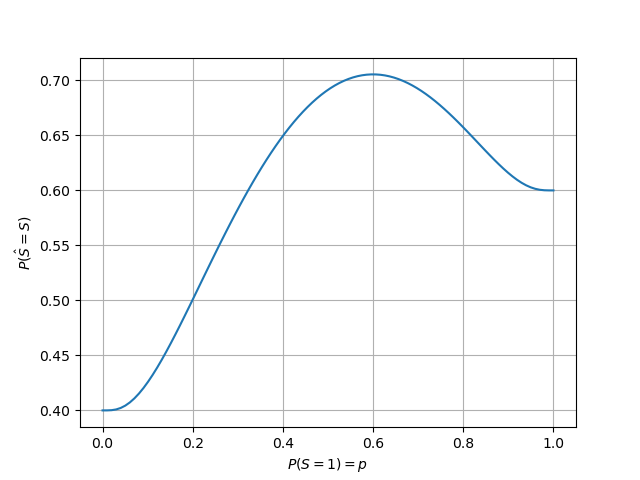
\includegraphics[width=0.8\linewidth]{elec-decoding-errors.png}
\caption{$\mathbb P(\hat S = S)$ for varying $p$.}
\end{figure}





% lecture 12: bias variance tradeoff
\section{Answers Lecture 12: Bias-Variance Tradeoff}

\paragraph{Question \ref{q:ridge_variance_reduction}}
We have the covariance of the ridge regression estimator as
\begin{equation*}
\BV(\lambda) = \mathbb{E}_{\mathbf{X}_{\text{train}}}[ \sigma^2 (\sigma^2 \lambda \mathbf{I} + \Phi^\top \Phi )^{-1} \Phi^\top \Phi (\sigma^2 \lambda \mathbf{I} + \Phi^\top \Phi )^{-1} ], \quad \BV(0) = \mathbb{E}_{\mathbf{X}_{\text{train}}}[ \sigma^2 ( \Phi^\top \Phi )^{-1} ].
\end{equation*}
Note that as we assume $\Phi^\top \Phi$ is invertible, we can rewrite
\begin{equation*}
\begin{aligned}
\BV(0) &= \mathbb{E}_{\mathbf{X}_{\text{train}}}[  \sigma^2 (\sigma^2 \lambda \mathbf{I} + \Phi^\top \Phi )^{-1} (\sigma^2 \lambda \mathbf{I} + \Phi^\top \Phi ) ( \Phi^\top \Phi )^{-1} (\sigma^2 \lambda \mathbf{I} + \Phi^\top \Phi ) (\sigma^2 \lambda \mathbf{I} + \Phi^\top \Phi )^{-1} ] \\
&= \mathbb{E}_{\mathbf{X}_{\text{train}}}[ \sigma^2 (\sigma^2 \lambda \mathbf{I} + \Phi^\top \Phi )^{-1} (2\sigma^2 \lambda \mathbf{I} + \sigma^4 \lambda^2 (\Phi^\top \Phi)^{-1} + \Phi^\top \Phi ) (\sigma^2 \lambda \mathbf{I} + \Phi^\top \Phi )^{-1} ].
\end{aligned}
\end{equation*}
So one can also show that:
\begin{equation*}
\BV(\lambda) - \BV(0) = \mathbb{E}_{\mathbf{X}_{\text{train}}}[ -\sigma^2 (\sigma^2 \lambda \mathbf{I} + \Phi^\top \Phi )^{-1} \underbrace{(2\sigma^2 \lambda \mathbf{I} + \sigma^4 \lambda^2 (\Phi^\top \Phi)^{-1} )}_{\text{positive definite}} (\sigma^2 \lambda \mathbf{I} + \Phi^\top \Phi )^{-1} ] \preceq 0,
\end{equation*}
To see why $2\sigma^2 \lambda \mathbf{I} + \sigma^4 \lambda^2 (\Phi^\top \Phi)^{-1}$ is positive definite: $\Psi^\top \Psi$ is positive semi-definite and invertible, so that $(\Psi^\top \Psi)^{-1}$ is positive definite, and scaling it with $\sigma^4 \lambda^2 > 0$ still maintain its positive definite property. Then the summation of two positive definite matrix ($2 \sigma^2 \lambda \mathbf{I}$ is positive definite) is a positive definite matrix, and the expectation of a positive definite matrix (as a random variable) still remains positive definite.

\paragraph{Question \ref{q:bias_variance_tradeoff_ridge_regression}}
We have the bias of the estimate is
\begin{equation*}
\Bb(\lambda) := \mathbb{E}_{\data \sim p_{data}^N}[\mparam^*_R(\data)] - \mparam_0 = - \mathbb{E}_{\mathbf{X}_{\text{train}}}[ \sigma^2 \lambda ( \sigma^2 \lambda \mathbf{I} + \Phi^\top \Phi )^{-1} ] \mparam_0,
\end{equation*}
This means:
\begin{equation*}
\Bb(\lambda) \Bb(\lambda)^\top = \mathbb{E}_{\mathbf{X}_{\text{train}}}[ \sigma^4 \lambda^2 ( \sigma^2 \lambda \mathbf{I} + \Phi^\top \Phi )^{-1} \mparam_0 \mparam_0^\top ( \sigma^2 \lambda \mathbf{I} + \Phi^\top \Phi )^{-1} ],
\end{equation*}
Using the result we have for $\BV(\lambda) - \BV(0)$ in Question \ref{q:ridge_variance_reduction}, we have:
\begin{equation*}
\Bb(\lambda) \Bb(\lambda)^\top + \BV(\lambda) - \BV(0) = - \mathbb{E}_{\mathbf{X}_{\text{train}}}[ \sigma^2 \lambda (\Phi^\top \Phi + \sigma^2 \lambda \mathbf{I})^{-1} \underbrace{(\sigma^2 [ 2 \mathbf{I} - \lambda \mparam_0 \mparam_0^\top + \sigma^2 \lambda (\Phi^\top \Phi)^{-1}] )}_{:= \mathbf{E}} (\Phi^\top \Phi + \sigma^2 \lambda \mathbf{I})^{-1} ].
\end{equation*} 
Furthermore, one can show that
\begin{equation*}
 \mathbf{E} \text{ is positive semi-definite } \quad \Leftrightarrow \quad \Bb(\lambda) \Bb(\lambda)^\top + \BV(\lambda) \preceq \BV(0),
\end{equation*}
which can be achieved by e.g.~setting $0 \leq \lambda \leq \frac{2}{|| \mparam_0 ||_2^2}$. To see this, a close inspection on $\mathbf{E}$ shows that if we make $2 \mathbf{I} - \lambda \mparam_0 \mparam_0^\top$ positive semi-definite then $\mathbf{E}$ will also be positive semi-definite. As $\mparam_0 \mparam_0^\top$ is a rank-1 matrix, the only non-zero eigenvalue of $\mparam_0 \mparam_0^\top$ is $|| \mparam_0 ||_2^2$. Using the discussed indications of eigen-decomposition, we can show that $2 \mathbf{I} - \lambda \mparam_0 \mparam_0^\top$ is positive semi-definite when all of its eigenvalues are non-negative, which can be achieved by $0 \leq \lambda \leq \frac{2}{|| \mparam_0 ||_2^2}$.

\paragraph{Question \ref{q:control_variate}}
(a) As $X$ is assumed to be an unbiased estimator of $x_0$, we have $\mathbb{E}_X[X] = x_0$. Now for the estimator $X + Y - \mathbb{E}_Y[Y]$:
$$\mathbb{E}_{X, Y}[ X + Y - \mathbb{E}_Y[Y] ] = \mathbb{E}_{X, Y}[X] + \mathbb{E}_{X, Y}[Y] - \mathbb{E}_Y[Y] = \mathbb{E}_{X}[X] = x_0,$$
therefore this estimator is also unbiased. 

(b) We compute the variance of this estimator:
\begin{equation*}
\begin{aligned}
\mathbb{V}_{X, Y}[ X + Y - \mathbb{E}_Y[Y] ] &= \mathbb{E}_{X, Y}[(X + Y - \mathbb{E}_Y[Y] - x_0 )^2] \\
&= \mathbb{E}_{X, Y}[( (X - \mathbb{E}_X[X]) + (Y - \mathbb{E}_Y[Y]) )^2] \\
&= \mathbb{E}_{X, Y}[(X - \mathbb{E}_X[X])^2 + (Y - \mathbb{E}_Y[Y])^2 + 2 (X - \mathbb{E}_X[X]) (Y - \mathbb{E}_Y[Y])] \\
&= \mathbb{V}_{X}[X] + \mathbb{V}_{Y}[Y] + 2 Cov_{X, Y}[X, Y].
\end{aligned}
\end{equation*}
This immediately implies that $\mathbb{V}_{X, Y}[ X + Y - \mathbb{E}_Y[Y] ] \leq \mathbb{V}_{X}[X]$ if $\mathbb{V}_{Y}[Y] + 2 Cov_{X, Y}[X, Y] < 0$.

(c) Following (b) and assume $Y = c Z$:
\begin{equation*}
\mathbb{V}_{X, Z}[ X + c Z - \mathbb{E}_Z[c Z] ] = \mathbb{V}_{X}[X] + c^2 \mathbb{V}_{Z}[Z] + 2c Cov_{X, Z}[X, Z].
\end{equation*}
To maximise variance reduction, we need to compute the derivative of $c^2 \mathbb{V}_{Z}[Z] + 2c Cov_{X, Z}[X, Z]$ w.r.t.~$c$ and make it equal to zero. This leads to:
$$ \frac{\partial}{\partial c} c^2 \mathbb{V}_{Z}[Z] + 2c Cov_{X, Z}[X, Z] = 2c \mathbb{V}_{Z}[Z] + 2 Cov_{X, Z}[X, Z] = 0 \quad \Rightarrow c = - \frac{Cov_{X, Z}[X, Z]}{\mathbb{V}_{Z}[Z]}.$$



% lecture 13: pca
\section{Answers Lecture 13: PCA}

\paragraph{Question \ref{q:pca_vs_linear_autoencoder}}
(a) Let us rewrite the objective $L(\BA, \BB)$:
\begin{equation*}
\begin{aligned}
L(\BA, \BB) :=& \frac{1}{N} \sum_{n=1}^N || \x_n - \BA \BB \x_n ||_2^2 = \frac{1}{N} \sum_{n=1}^N (\x_n - \BA \BB \x_n)^\top (\x_n - \BA \BB \x_n) \\
=& \frac{1}{N} \sum_{n=1}^N (\x_n^\top \x_n - 2 \x_n^\top \BA \BB \x_n + \x_n^\top \BB^\top \BA^\top \BA \BB \x_n) \\
=& \frac{1}{N} \sum_{n=1}^N (\x_n^\top \x_n - 2 \tr(\x_n^\top \BA \BB \x_n) + \tr(\x_n^\top \BB^\top \BA^\top \BA \BB \x_n)) \\
=& \frac{1}{N} \sum_{n=1}^N (\x_n^\top \x_n - 2 \tr(\BA \BB \x_n \x_n^\top ) + \tr(\BB^\top \BA^\top \BA \BB \x_n x_n^\top )) \\
=& \frac{1}{N} \sum_{n=1}^N (\x_n^\top \x_n - 2 \tr(\BA \BB \x_n \x_n^\top ) + \tr(\BB^\top \BA^\top \BA \BB \x_n x_n^\top )) \\
=& \frac{1}{N} \sum_{n=1}^N \x_n^\top \x_n - 2 \tr(\BA \BB \frac{1}{N} \underbrace{\sum_{n=1}^N \x_n \x_n^\top}_{:=\BS} ) + \tr(\BB^\top \BA^\top \BA \BB \frac{1}{N} \sum_{n=1}^N \x_n x_n^\top ) \\
=& \frac{1}{N} \sum_{n=1}^N \x_n^\top \x_n - 2 \tr(\BA \BB \BS ) + \tr(\BB^\top \BA^\top \BA \BB \BS )
\end{aligned}
\end{equation*}
Now we derive the derivative of $L(\BA, \BB)$ w.r.t.~$\BA$, and notice that $ \tr(\BB^\top \BA^\top \BA \BB \BS ) =  \tr(\BA^\top \BA \BB \BS \BB^\top )$:
\begin{equation*}
\frac{\partial}{\partial \BA} L = 2 \BA \BB \BS \BB^\top - 2 \BS \BB^\top.
\end{equation*}
Similarly we derive the derivative of $L(\BA, \BB)$ w.r.t.~$\BB$:
\begin{equation*}
\frac{\partial}{\partial \BB} L = 2 \BA^\top \BA \BB \BS - 2 \BA^\top \BS.
\end{equation*}

(b) As we assume $rank(\BA) = M$, $\BA^\top \BA$ is invertible. As $\BS$ is also assumed to be invertible, then the optimal solution of $\BB^*$ satisfies:
$$ \BA^\top \BA \BB^* \BS =\BA^\top \BS \quad \Rightarrow \quad  \BA^\top \BA \BB^* =\BA^\top \quad \Rightarrow \quad \BB^* = (\BA^\top \BA)^{-1} \BA^\top.$$

(c) We first consider, when $\BB$ is a given rank-$M$ matrix, the optimal solution of $\BA^*$ satisfies:
$$ \BA^* \BB \BS \BB^\top = \BS \BB^\top \quad \Rightarrow \quad \BA^* = \BS \BB^\top (\BB \BS \BB^\top)^{-1}.$$
Combining (b), this means the optimal solution $\BA^*, \BB^*$ satisfies:
$$ \BA^* = \BS (\BB^*)^\top (\BB^* \BS (\BB^*)^\top)^{-1}, \quad \BB^* = ((\BA^*)^\top \BA^*)^{-1} (\BA^*)^\top.$$

Note that $\BB \BS \BB^\top$ is invertible because both $\BB$ and $\BS$ has full row rank. Now writing $\BS = \BQ \Lambda \BQ^\top$, we verify in below that $\BA^* = \BQ_{1:M}, \BB^* = \BQ_{1:M}^{\top}$ is a fixed point of the objective $L(\BA, \BB)$.
\begin{equation*}
\begin{aligned}
\BS (\BB^*)^\top (\BB^* \BS (\BB^*)^\top)^{-1} &= \BQ \Lambda \BQ^\top \BQ_{1:M} (\BQ_{1:M}^{\top} \BQ \Lambda \BQ^\top \BQ_{1:M})^{-1} \\
&= \BQ \Lambda \begin{bmatrix} \mathbf{I}_{M} & 0 \\ 0 & 0 \end{bmatrix} \left( \begin{bmatrix} \mathbf{I}_{M} & 0 \\ 0 & 0 \end{bmatrix} \Lambda \begin{bmatrix} \mathbf{I}_{M} & 0 \\ 0 & 0 \end{bmatrix} \right)^{-1} \\
&= \BQ \Lambda \begin{bmatrix} \Lambda_{1:M}^{-1} & 0 \\ 0 & 0 \end{bmatrix} = \BQ \begin{bmatrix} \mathbf{I}_{M} & 0 \\ 0 & 0 \end{bmatrix} = \BQ_{1:M} = \BA^*,
\end{aligned}
\end{equation*}
%
\begin{equation*}
((\BA^*)^\top \BA^*)^{-1} (\BA^*)^\top = (\BQ_{1:M}^\top \BQ_{1:M})^{-1} \BQ_{1:M}^\top = \BQ_{1:M}^\top = \BB^*.
\end{equation*}
In general a fixed point of the objective satisfies:
$$ \BA^* = \BQ_{1:M} \BC^{-1}, \BB^* = \BC \BQ_{1:M}^{\top}, \quad \forall \text{ invertible matrix } \BC \in \mathbb{R}^{M \times M}.$$


\paragraph{Question \ref{q:svd_and_pca}}
Let us write an SVD of $\X$ as $\X = \BU \Sigma \BV^\top$ with $\BU \in \mathbb{R}^{N \times N}, \Sigma \in \mathbb{R}^{N \times D}$ and $\BV \in \mathbb{R}^{D \times D}$. Note that the covariance on $\mathcal{D}$ can be computed as $\BS = \BX^\top \BX$. Plugging in the SVD of $\X$:
$$ \BS = \BX^\top \BX = \BV \Sigma^{\top} \BU^\top \BU \Sigma \BV^\top = \BV \Sigma^{\top} \Sigma \BV^\top.$$
Note that in an SVD, $\Sigma$ is a rectangular diagonal matrix, i.e., only the leading diagonal terms have non-zero values. This also means $\Sigma^{\top} \Sigma \in \mathbb{R}^{D \times D}$ is a diagonal matrix with non-negative diagonal values. Therefore $\BV \Sigma^{\top} \Sigma \BV^\top$ is an eigendecomposition of $\BS$, therefore by sorting the diagonal values in $\Sigma^{\top} \Sigma$ in descending order, we can retrieve the corresponding columns in $\BV$ as the principal components.


\section{Answers Lecture 14: Probabilistic PCA}

\paragraph{Question \ref{q:optimal_prob_pca}}
(a) As shown in the lecture, the optimal $\BW^*$ with its SVD $\BW^* = \BU \Sigma \BV^\top$ satisfies
$$(\BS \bm{u}_1, ..., \BS \bm{u}_M, \bm{0}, ..., \bm{0}) = ((\sigma_1^2 + \sigma^2) \bm{u}_1, ..., (\sigma_M^2 + \sigma^2) \bm{u}_M, \bm{0}, ..., \bm{0}), \quad \sigma_m = \Sigma_{mm}$$
Plugging-in $\BS = \BQ \Lambda \BQ^\top$, the above equation means $\bm{u}_m = \bm{q}_{i_m}, 1 \leq i_m \leq D$ for $i = 1, ..., M$. Also due to the orthogonality constraint of $\BU$ column vectors (by definition of SVD), we know that $\{ i_m \}_{m=1}^M$ contains distinct indices. This leads to:
\begin{equation*}
\BS \bm{u}_m = \lambda_{i_m} \bm{q}_{i_m} = (\sigma_m^2 + \sigma^2) \bm{q}_{i_m}.
\end{equation*}
which proves statement (a). 

(b) We first compute $\BC = \BW \BW^\top + \sigma^2 \mathbf{I}$ for $\BW^*$ using SVD of $\BW$:
\begin{equation*}
\begin{aligned}
\BC &= \BU
\begin{bmatrix} 
    \sigma_{1} & 0 & \dots \\
    0 & \ddots & \\
    \vdots &        & \sigma_M \\ 
     &   & 0 \\
     & & \vdots \\
     & & 0
    \end{bmatrix} \BV^\top \BV 
    \begin{bmatrix} 
    \sigma_{1} & 0 & \dots \\
    0 & \ddots & \\
    \vdots &        & \sigma_M \\ 
     &   & 0 \\
     & & \vdots \\
     & & 0
    \end{bmatrix}^\top \BU^\top + \sigma^2 \mathbf{I} \\
&= \BU
\begin{bmatrix} 
    \sigma_{1}^2 + \sigma^2 & 0 & \dots \\
    0 & \ddots & \\
    \vdots &        & \sigma_M^2 + \sigma^2 \\ 
     &   &  & \sigma^2 \\
     & & & & \ddots & \\
     & & & & &  \sigma^2
    \end{bmatrix} \BU^\top
\end{aligned}
\end{equation*}

Plugging-in the optimal $\bm{\mu}^*$ and a fixed point of $\BW^*$ from (a): 
\begin{equation*}
\begin{aligned}
\BC &= (\bm{q}_{i_1}, ..., \bm{q}_{i_M}, \bm{u}_{M+1}, ..., \bm{u}_D)
\begin{bmatrix} 
    \lambda_{i_1} & 0 & \dots \\
    0 & \ddots & \\
    \vdots &        & \lambda_{i_M} \\ 
     &   &  & \sigma^2 \\
     & & & & \ddots & \\
     & & & & &  \sigma^2
    \end{bmatrix} (\bm{q}_{i_1}, ..., \bm{q}_{i_M}, \bm{u}_{M+1}, ..., \bm{u}_D)^\top,
\end{aligned}
\end{equation*}
which satisfies $\log |C| = (D - M) \log \sigma^2 + \sum_{m=1}^M \log \lambda_{i_m}$. Notice that the above equation returns the same matrix for $\BC$ no matter how we choose $\bm{u}_{M+1}, ..., \bm{u}_D$ as long as $\BU$ contains an orthonormal basis (by definition of SVD). This means for $m \geq M+1$ we can simply choose $\bm{u}_m = \bm{q}_j$ for some $j \notin \{ i_1, i_2, ..., i_M \}$. Therefore with such choices of $\bm{u}_{M+1}, ..., \bm{u}_D$, there exists a permutation matrix $\BP$ such that $\BU = \BQ \BP$ which gives the corresponding permutation of the $\BQ$ basis vectors. 
Then the corresponding MLE objective is:
\begin{equation*}
\begin{aligned}
\log p_{\mparam^*}(\x) &= \log \mathcal{N}(\x; \bm{\mu}^*,  \BC), \quad \BC = \BQ \BP (\Sigma \Sigma^\top + \sigma^2 \mathbf{I}) \BP^\top \BQ^\top \\
\Rightarrow \quad \mathcal{L}(\mparam^*) &= \frac{1}{N} \sum_{n=1}^N \log \mathcal{N}(\x_n; \bm{\mu}^*,  \BC) \\
&= -\frac{D}{2} \log 2\pi -\frac{1}{2} \log |\BC| - \frac{1}{2} \frac{1}{N} \sum_{n=1}^N (\x_n - \bm{\mu}^*)^\top \BC^{-1} (\x_n - \bm{\mu}^*) \\
&= -\frac{D}{2} \log 2\pi -\frac{1}{2} \log |\BC| - \frac{1}{2} \tr( \BC^{-1} \frac{1}{N} \sum_{n=1}^N (\x_n - \bm{\mu}^*)(\x_n - \bm{\mu}^*)^\top) \\
&= -\frac{D}{2} \log 2\pi -\frac{1}{2} \log |\BC| - \frac{1}{2} \tr( \BC^{-1} \BS) \\
&= -\frac{D}{2} \log 2\pi -\frac{1}{2} \log |\BC| - \frac{1}{2} \tr( \BQ \BP (\Sigma \Sigma^\top + \sigma^2 \mathbf{I})^{-1} \BP^\top \BQ^\top \BQ \Lambda \BQ^\top) \\
&= -\frac{D}{2} \log 2\pi -\frac{1}{2} \log |\BC| - \frac{1}{2} \tr(  \BP (\Sigma \Sigma^\top + \sigma^2 \mathbf{I})^{-1} \BP^\top \Lambda \BQ^\top \BQ) \\
&=  -\frac{D}{2} \log 2\pi -\frac{1}{2} \log |\BC| - \frac{1}{2} \tr( (\Sigma \Sigma^\top + \sigma^2 \mathbf{I})^{-1} \BP^\top \Lambda \BP )
\end{aligned}
\end{equation*}
We have used permutation invariance of matrix trace. Under the condition in question (a) and the property that $\BP^\top \Lambda \BP$ permutes the diagonals of $\Lambda$ using the permutation defined by $\BP$, we can show that the top-left $M \times M$ blocks of $(\BP^{-1} \Lambda \BP)$ and $(\Sigma \Sigma^{\top} + \sigma^2 \mathbf{I})$ are equal. This means we only need to consider the last $M+1$ to $D$ diagonal terms in $(\Sigma \Sigma^\top + \sigma^2 \mathbf{I})^{-1} \BP^{-1}  \Lambda \BP$ for the trace term, which reads:
$$\tr( (\Sigma \Sigma^\top + \sigma^2 \mathbf{I})^{-1} \BP^{-1}  \Lambda \BP) = M + \sigma^{-2} \sum_{j \not \in \{i_1, ..., i_M \}} \lambda_j.$$
%
Also recall that $\log |C| = (D - M) \log \sigma^2 + \sum_{m=1}^M \log \lambda_{i_m}$. Combining both results, this means we would like to find an permutation mapping $\rho(\cdot)$ to minimise
\begin{equation*}
\begin{aligned}
\log |\BC | + \tr( \BC^{-1} \BS) &=  M + \sigma^{-2} \sum_{j \not \in \{i_1, ..., i_M \}} \lambda_j + \sum_{m=1}^M \log \lambda_{i_m} + (D - M) \log \sigma^2 \\
&= M + \sum_{j \not \in \{i_1, ..., i_M \}} \frac{ \lambda_j}{\sigma^2} + \sum_{m=1}^M \log \frac{ \lambda_{i_m}}{\sigma^2} + D \log \sigma^2.
\end{aligned}
\end{equation*}
%
Recall the assumption of descending eigenvalues $\lambda_1 \geq ... \geq \lambda_D \geq 0$. Since we can show that $x > \log x$ (natural logarithm) for all $x > 0$, then to minimise the above expression, we want to use larger eigenvalues for the $\log \frac{ \lambda_{i_m}}{\sigma^2}$ terms and smaller eigenvalues for the $\frac{ \lambda_j}{\sigma^2}$ terms. This means the global maximum solutions satisfy $i_m = m$ for $m = 1, ..., M$.


\printbibliography

\end{document}
